% ------------------------------------------------------------------
\documentclass[12 pt]{article} % A4 paper set by geometry package below
\pagenumbering{arabic}
\setlength{\parindent}{10 mm}
\setlength{\parskip}{12 pt}

% Nimbus Sans font should be reasonably legible
\usepackage{helvet}
\renewcommand{\familydefault}{\sfdefault}
\usepackage[T1]{fontenc}  % Without this \textsterling produces $

% Section header spacing
\usepackage{titlesec}
\titlespacing\section{0pt}{12pt plus 4pt minus 2pt}{0pt plus 2pt minus 2pt}
\titlespacing\subsection{0pt}{12pt plus 4pt minus 2pt}{0pt plus 2pt minus 2pt}
\titlespacing\subsubsection{0pt}{12pt plus 4pt minus 2pt}{0pt plus 2pt minus 2pt}

\usepackage{amsmath}
\usepackage{amssymb}
\usepackage{graphicx}
\usepackage{verbatim}    % For comment
\usepackage[paper=a4paper, marginparwidth=0 cm, marginparsep=0 cm, top=2.5 cm, bottom=2.5 cm, left=3 cm, right=3 cm, includemp]{geometry}
\usepackage[pdftex, pdfstartview={FitH}, pdfnewwindow=true, colorlinks=true, citecolor=blue, filecolor=blue, linkcolor=blue, urlcolor=blue, pdfpagemode=UseNone]{hyperref}

\usepackage{framed,color}
\usepackage{fancybox}
\usepackage{varwidth}
\definecolor{shadecolor}{rgb}{1,0.8,0.3}
\usepackage[framemethod=tikz]{mdframed}

% To highlight revisions in pdf
\usepackage[normalem]{ulem}
\definecolor{green}{rgb}{0,0.4,0}
\newcommand{\rem}[1]{\textcolor{red}{\sout{#1}}}
\newcommand{\add}[1]{\textcolor{green}{\uwave{#1}}}

% Put module code and last-modified date in footer
\usepackage{fancyhdr}
\pagestyle{fancy}
\fancyhf{}
\renewcommand{\headrulewidth}{0pt}
\cfoot{{\small \thisweek}\hfill \thepage\hfill {\small \moddate}}

% Hopefully address Canvas complaints about pdf tagging
%\usepackage[tagged]{accessibility}
% ------------------------------------------------------------------



% ------------------------------------------------------------------
% Shortcuts
\newcommand{\cE}{\ensuremath{\mathcal E} }
\newcommand{\cF}{\ensuremath{\mathcal F} }
\newcommand{\khat}{\ensuremath{\widehat k} }
\newcommand{\Nbb}{\ensuremath{\mathbb N} }
\newcommand{\cO}{\ensuremath{\mathcal O} }
\newcommand{\Rbb}{\ensuremath{\mathbb R} }
\newcommand{\Sbar}{\ensuremath{\overline S} }
\newcommand{\vdr}{\ensuremath{v_{\mathrm{dr}}} }
\newcommand{\Xbar}{\ensuremath{\overline X} }
\newcommand{\al}{\ensuremath{\alpha} }
\newcommand{\be}{\ensuremath{\beta} }
\newcommand{\De}{\ensuremath{\Delta} }
\newcommand{\de}{\ensuremath{\delta} }
\newcommand{\la}{\ensuremath{\lambda} }
\newcommand{\lath}{\ensuremath{\la_{\mathrm{th}}} }
\newcommand{\si}{\ensuremath{\sigma} }
\newcommand{\om}{\ensuremath{\omega} }
\newcommand{\Om}{\ensuremath{\Omega} }
\newcommand{\lra}{\ensuremath{\longrightarrow} }
\newcommand{\Lra}{\ensuremath{\Longrightarrow} }
\newcommand{\llra}{\ensuremath{\longleftrightarrow} }
\newcommand{\X}{\ensuremath{\!\times\!} }
\newcommand{\vev}[1]{\ensuremath{\left\langle #1 \right\rangle} }
\newcommand{\pderiv}[2]{\ensuremath{\frac{\partial #1}{\partial #2}} }
\newcommand{\eq}[1]{Eq.~\ref{#1}}
\newcommand{\fig}[1]{Figure~\ref{#1}}
\newcommand{\secref}[1]{Section~\ref{#1}}
\newcommand{\TODO}[1]{\textcolor{red}{\textbf{#1}}}
% ------------------------------------------------------------------



% ------------------------------------------------------------------
\begin{document}
\thispagestyle{empty}
\begin{center}
  {\LARGE \textbf{MATH327: Statistical Physics}} \\[6 pt]
  \textbf{David Schaich \qquad\qquad\qquad\qquad Spring 2021} \\[48 pt]
  {\LARGE LECTURE \ NOTES} \\[6 pt]
  Last modified 4 March 2021
\end{center}
\renewcommand{\contentsname}{}
\setcounter{tocdepth}{1}
\tableofcontents
% ------------------------------------------------------------------



% ------------------------------------------------------------------
\newpage
% ------------------------------------------------------------------
\newcommand{\thisweek}{MATH327 information}
\newcommand{\moddate}{Last modified 4 Feb.~2021}
\setcounter{section}{0}
\phantomsection
\addcontentsline{toc}{section}{Module information and logistics}
\section*{Module information and logistics}

\subsection*{Coordinator}
\begin{description}
  \setlength{\itemsep}{1pt}
  \setlength{\parskip}{0pt}
  \setlength{\parsep}{0pt}
  \item[\qquad] Dr David Schaich
  \item[\qquad] Mathematics Building Room 124 (Theoretical Physics Wing)
  \item[\qquad] \href{mailto:david.schaich@liverpool.ac.uk}{david.schaich@liverpool.ac.uk}
  \item[\qquad] \href{http://www.davidschaich.net}{www.davidschaich.net}
\end{description}
% ------------------------------------------------------------------



% ------------------------------------------------------------------
\subsection*{Weekly schedule}
\textbf{Synchronous sessions} are timetabled at 9:00 on Mondays and 13:00 on Thursdays.

\textbf{Office hours} will take place immediately afterwards, at 10:00 on Mondays and 14:00 on Thursdays.
If these times do not work with your schedule, you can also make an appointment through \href{https://calendly.com/daschaich}{calendly.com/daschaich}.
% ------------------------------------------------------------------



% ------------------------------------------------------------------
\subsection*{Delivery plans and module resources}
Redesigning this module for remote delivery requires some experimentation and improvisation, so you should feel free to make requests and suggestions regarding how the module may best be delivered.
In order to ensure that the amount of material remains manageable, we will cover the same content as last year's edition of the module, rewriting it for remote learning in place of in-person lectures and computer labs.
All resources for the module will be collected at \href{https://liverpool.instructure.com/courses/19478}{its Canvas site}, \\
\centerline{\href{https://liverpool.instructure.com/courses/19478}{liverpool.instructure.com/courses/19478}}

I will aim to minimize the number of announcements sent to you through Canvas.
You have the option to receive email notification of these announcements.
If you choose to turn off these email notifications, you should make sure to check Canvas regularly for announcements.
I will assume announcements have been read within 24 hours.

\subsubsection*{Lecture notes}
We will use the \textit{Notes-driven Asynchronous Delivery} framework designed by the Department of Mathematical Sciences, in which the primary learning materials are the lecture notes you are currently reading.
As you read further, you will encounter \textbf{gaps} in the notes where you will be able to check your understanding by completing some exercises that are intended to be bite-sized.
Feel free to complete these exercises in whatever format you find most convenient, for instance on separate pieces of paper.
While the size of the gap is intended to indicate the rough scale of the exercise, your work may or may not fit depending on your handwriting and solution strategy.

You will also see many numbered equations in the lecture notes.
In general, equations are numbered so that they can easily be referred to in subsequent discussions, derivations or examples.
Therefore a number is not necessarily an indication of importance.
Some particularly important results, definitions and concepts will be highlighted by coloured boxes.
You should ensure you understand the key learning objectives in these coloured boxes.
There is no need to memorize any equations.

\subsubsection*{Synchronous sessions}
These gaps will guide our twice-weekly synchronous sessions using Zoom on Monday mornings and Thursday afternoons.
In addition to discussing any general questions you may have, we will aim to complement the asynchronous material by focusing our attention on any gaps that proved challenging to fill.
In order for these synchronous sessions to remain in \textbf{active learning} mode, you may be asked to describe your own approach to any given gap.
Thinking about them in advance will make this easier.
If you get stuck during the synchronous session, I will aim to ask leading questions rather than lecturing.

\subsubsection*{Video recordings and asynchronous discussions}
To supplement these lecture notes, the Department's delivery framework also involves regular video recordings, expected to add up to around 20 minutes per week.
For each week I plan to provide both an introductory video presenting big-picture context and motivation for the week's topic, followed by a concluding summary of the key results to take away as learning outcomes.
Since \textbf{synchronous sessions will not be recorded}, to encourage your participation, I also expect to add supplemental videos addressing any particularly tricky issues that arise in the course of those synchronous sessions (for example, working through gaps that prove challenging).
Supplemental exercises may also be released to respond to particular challenges we encounter.
The Canvas site also provides a \textit{\href{https://liverpool.instructure.com/courses/19478/discussion_topics}{Discussion}} utility where questions can be asked, discussed and answered asynchronously.

\subsubsection*{Term schedule and organization}
The planned schedule for the module is summarized on the first page of these notes.
If necessary to respond to unanticipated challenges, there should be some flexibility to adapt this schedule.
The amount and difficulty of material necessarily fluctuate from week to week, and different material may prove more or less difficult to different students.
Sticking with the same content as last year should ensure that these fluctuations average out over the course of the term.

This content is organized around the concept of \textit{statistical ensembles} introduced by \href{https://en.wikipedia.org/wiki/Josiah_Willard_Gibbs}{J.\ Willard Gibbs} in the early 1900s.
In essence, a statistical ensemble is a mathematical framework for concisely describing the properties of (idealized) physical systems with a large number of independent objects, subject to certain constraints.
After a week studying the mathematical foundations underlying these frameworks, we will learn about the \textit{micro-canonical ensemble} in week 2 and the \textit{canonical ensemble} in week 3.
We will spend weeks 4 and 5 on applications of the canonical ensemble, first considering ideal gases and then investigating thermodynamic cycles.
In week 6 we will see our third and final statistical ensemble, the \textit{grand-canonical ensemble}, which we will apply to various types of quantum gases in weeks 7--9.
Those first nine weeks will all consider systems whose constituent objects do not interact with each other.
We will explore effects of interactions in week 10, which opens up a much broader landscape of applications that we will survey for the remainder of the term (along with some overall synthesis and review to help prepare for the final assessment).

The asynchronous materials for each week will be available through Canvas at least a week in advance.
For example, the notes and videos for week 1 (8--15 February) will be available on or before Sunday, 31 January.
In case subsequent corrections or additions to the notes are needed, the date of last modification will be included at the bottom of each page.

\subsubsection*{Version control and co-creation}
An easy way to check any corrections or additions that may need to be made to these notes is provided by the public GitHub repository where their \LaTeX\ source is maintained under version control: \\
\centerline{\href{https://github.com/daschaich/MATH327_2021}{github.com/daschaich/MATH327\_2021}}
In addition, you are also welcome to use GitHub to report issues with the notes\footnote{Questions about the mathematical content should go to the Canvas discussions.} and create pull requests to address them.
% Captions for the video recordings will also be maintained in this repository.
Such co-creation is entirely optional.
If you are interested in learning more about version control with \texttt{git}, the \href{https://software-carpentry.org}{Software Carpentry} project provides free resources at \\
\centerline{\href{https://swcarpentry.github.io/git-novice/}{swcarpentry.github.io/git-novice/}}

\subsubsection*{Expected background}
You may have seen quantum statistics and quantum gases listed in the module schedule on the first page, so I will emphasize that no prior knowledge of quantum mechanics is assumed.
Any necessary information on this topic will be provided.
%
It is also not necessary to be familiar with statistical analysis or combinatorics.
In those contexts I just anticipate that you have previously seen the \href{https://en.wikipedia.org/wiki/Standard_deviation}{standard deviation} and the \href{https://en.wikipedia.org/wiki/Binomial_coefficient}{binomial coefficient}
\begin{equation*}
  \binom{N}{k} = \frac{N!}{k! \, (N - k)!} = \binom{N}{N - k}
\end{equation*}
that counts the number of possible ways to choose $k$ objects out of a set of $N \geq k$ total objects.
I also anticipate that you have previously seen \href{https://en.wikipedia.org/wiki/Gaussian_integral}{gaussian integrals},
\begin{equation*}
  \int_{-\infty}^{\infty} e^{-a (x + b)^2} = \sqrt{\frac{\pi}{a}}.
\end{equation*}
% ------------------------------------------------------------------



% ------------------------------------------------------------------
\subsection*{Assessment and academic integrity}
The assessment workload has also been kept the same as last year, though weights have been distributed more evenly across the term to accommodate current circumstances and avoid a high-stakes final assessment.
Deadlines for in-term assignments have been coordinated within the Department to minimize pile-up.
MATH327 has been allocated the following deadlines at 23:59 on \textbf{Tuesdays}:
\begin{description}
  \item[20\%] A computer-based project divided into two equally weighted parts, the first due \textbf{Tuesday, 2 March} and the second due \textbf{Tuesday, 13 April}
  \item[15\%] A homework assignment available by Monday, 22 February and due \textbf{Tuesday, 16 March}
  \item[15\%] A homework assignment available by Monday, 19 April and due \textbf{Tuesday, 27 April}
  \item[50\%] A final assessment to be centrally scheduled within the period 17 May through 4 June
\end{description}
Since the second part of the computer project is due shortly after the term break, feedback for the first part will be provided before the break, and office hours will continue during the break in case any assistance is needed with this project.

Following the University's \href{https://www.liverpool.ac.uk/media/livacuk/tqsd/aqsd/code_of_practice_on_assessment.pdf}{Code of Practice on Assessment}, late submissions completed within five days (120 hours) after the submission deadline will have 5\% of the total marks deducted for each 24-hour post-deadline period.
Submissions more than five days late will be awarded zero marks, though I will still endeavour to provide feedback on them.
I will aim to return feedback and solutions 7--10 days after the deadline.

Because the computer-based project will be done remotely, rather than in a computer lab on campus, you are free to complete it using the programming language of your choice.
Instruction on the necessary programming concepts will be provided using \href{https://www.python.org}{Python}, the free programming language recommended for the project.
If you have difficulty setting up Python on your device, you can run it for free online at \href{https://repl.it/languages/python3}{repl.it}.
(Make sure to keep a copy of the code to submit for assessment!)
Alternative languages could include \href{https://en.wikipedia.org/wiki/C_(programming_language)}{C}, \href{https://www.r-project.org}{R}, or even \href{https://matlab.mathworks.com}{MATLAB} (through the University's site license).
Maple may struggle to handle parts of the project.

I encourage you to discuss the in-term assignments with each other, since discussing and debating concepts and procedures is a very effective way to learn.
The examination must be done on your own, and your submissions for all assignments must be your own work representing your own understanding.
Clear and neat presentations of your workings and the logic behind them will contribute to your mark.
It is unacceptable to copy solutions in part or in whole from other students (current or prior) or from other sources (commercial or otherwise).
Should you make use of resources beyond the module materials, these must be explicitly referenced in your work.

By now you should have successfully passed the Academic Integrity Tutorial and Quiz to affirm that you have read and understood the Academic Integrity Policy detailed in Appendix L of the Code of Practice on Assessment.
If you have any questions about what is or is not acceptable under this policy, please ask me or Departmental Assessment Officer Kamila Zychaluk.
In all cases, the spirit of the Academic Integrity Policy should take precedence over legalistic convolutions of the text.
% ------------------------------------------------------------------



% ------------------------------------------------------------------
\subsection*{Additional resources}
The lists of further reading below provide some optional additional resources that may be helpful.
Hyperlinks lead either to the resource itself or to the corresponding record page in our library.

\noindent\textbf{Books and lecture notes at roughly the level of this module:} \\[-24 pt]
\begin{enumerate}
  \item David Tong, \href{https://www.damtp.cam.ac.uk/user/tong/statphys.html}{\textit{Lectures on Statistical Physics}} (2012), \\ www.damtp.cam.ac.uk/user/tong/statphys.html
  \item Daniel V.~Schroeder, \textit{An Introduction to Thermal Physics} (first edition, 2000)
  \item C.~Kittel and H.~Kroemer, \textit{Thermal Physics} (second edition, 1980)
  \item F.~Reif, \textit{Fundamentals of Statistical and Thermal Physics} (first edition, 1965)
\end{enumerate}

\noindent\textbf{More advanced and more specialized books}, which may be useful to consult concerning specific questions or topics: \\[-24 pt]
\begin{enumerate}
  \setcounter{enumi}{4}
  \item R.~K.~Pathria, \textit{Statistical Mechanics} (second edition, 1996)
  \item Sidney Redner, \textit{A Guide to First-Passage Processes} (first edition, 2007)
  \item Pavel L.~Krapivsky, Sidney Redner and Eli Ben-Naim, \textit{A Kinetic View of Statistical Physics} (first edition, 2010)
  \item Kerson Huang, \textit{Statistical Mechanics} (second edition, 1987)
  \item Weinan E, Tiejun Li and Eric Vanden-Eijnden, \textit{Applied Stochastic Analysis} (first edition, 2019)
  \item Michael Plischke and Birger Bergersen, \textit{Equilibrium Statistical Physics} (third edition, 2005)
  \item L.~D.~Landau and E.~M.~Lifshitz, \textit{Statistical Physics, Part 1} (third edition, 1980)
\end{enumerate}

\newpage % WARNING: FORMATTING BY HAND
\noindent\textbf{A general book about learning}, which (among other strategies) emphasizes the value of retrieval practice compared to re-reading lecture notes or re-watching videos: \\[-24 pt]
\begin{enumerate}
  \setcounter{enumi}{11}
  \item Peter C.~Brown, Henry L.~Roediger III and Mark A.~McDaniel, \textit{Make it Stick: The Science of Successful Learning} (first edition, 2014) \\
        A \href{https://www.youtube.com/watch?v=MfylloWuuZU}{short summary video} is also available
\end{enumerate}

\noindent\textbf{Maple and MATLAB resources:} \\[-24 pt]
\begin{enumerate}
  \setcounter{enumi}{12}
  \item Ian Thompson, \href{https://library.liv.ac.uk/record=b4395758~S8}{\textit{Understanding Maple}} (ebook edition, 2017) \\
        Related videos: \href{https://stream.liv.ac.uk/4k67bdzt}{\textit{Running Maple for the first time}} (stream.liv.ac.uk/4k67bdzt) \\
        \textcolor{white}{Related videos:} \href{https://stream.liv.ac.uk/7pjge23a}{\textit{Configuring Maple}} (stream.liv.ac.uk/7pjge23a)
  \item Stormy Attaway, \textit{MATLAB: A Practical Introduction to Programming and Problem Solving} (third edition, 2013)
  \item B.~Barnes and G.~R.~Fulford, \textit{Mathematical Modelling with Case Studies: Using Maple and MATLAB} (third edition, 2014)
\end{enumerate}

Finally, there is a vast constellation of purely online resources, such as \href{https://en.wikipedia.org/wiki/Statistical_physics}{Wikipedia}.
These are often fine places to \emph{start} learning about a subject, but may be terrible places to \emph{stop}.
% ------------------------------------------------------------------


\newpage
% ------------------------------------------------------------------
\renewcommand{\thisweek}{MATH327 Week 1}
\renewcommand{\moddate}{Last modified 15 Jan.~2021}
\setcounter{section}{1}
\section*{Week 1: Central limit theorem and diffusion}
\addcontentsline{toc}{section}{Week 1: Central limit theorem and diffusion}

\subsection*{Introductory remarks: What is Statistical Physics?}
Mathematical sciences such as physics aim to determine the laws of nature and understand how these govern experimental observations---both in everyday circumstances and under extreme conditions.
This mathematical understanding is typically guided by reproducing a set of observations, with the resulting framework then used to make predictions for other ``observables''.

Over the past few centuries this process has been tremendously successful, with theoretical physics accurately predicting experimental and observational results from sub-atomic through to extra-galactic scales.
Modern physics labs can create a vacuum better than in outer space and the coldest temperatures in the known universe, as well as going to the other extreme to reach temperatures of millions of degrees and pressures millions of times atmospheric pressure at sea level.
Amazingly, many aspects of these realms of physics can be theoretically described by mathematics developed centuries ago.\footnote{Eugene Wigner's famous article, ``\href{https://en.wikipedia.org/wiki/The_Unreasonable_Effectiveness_of_Mathematics_in_the_Natural_Sciences}{The Unreasonable Effectiveness of Mathematics in the Natural Sciences}'' (1960), and subsequent work in the philosophy of physics, elaborates on why this may be considered `amazing'.  These lecture notes will not comment extensively on philosophy.}

The domain of \textbf{statistical physics} is one in which simple mathematical principles enable amazing predictive capabilities.
Initially developed in the nineteenth century, statistical physics remains a core component of modern physics, and will retain this position in years to come.
The foundations of statistical physics lie in the use of probability theory to mathematically describe experimental observations and corresponding laws of nature that involve stochastic randomness rather than being perfectly predictable.

The lack of perfect predictability in statistical physics is a matter of practicality rather than one of principle.
It results from working with a large number of degrees of freedom (i.e., a large number of independent objects such as particles or balls).
For example, Avogadro's number $N_A \approx 6.022\times 10^{23}$ is the large number of molecules in everyday amounts of familiar substances---about 18~grams of water or about 22~litres of air at sea-level atmospheric pressure ($\approx$$101$~kPa). % 22.4 litres for 1atm=101.325~kPa, 22.71 litres for 100~kPa at $O^{\circ}$~C
Specifying the positions and velocities of $\sim$$10^{23}$ objects would require far more information than could be stored even in the memory of the biggest existing supercomputers.
Statistical physics instead produces simple mathematical descriptions of large-scale properties such as temperature, pressure and diffusion, which are generally of such outstanding quality that the underlying `randomness' is effectively undetectable.

Historically, the difficulty detecting the stochastic processes underlying such \textit{thermodynamic} properties made it challenging to convince skeptics that atoms and molecules really exist.
Ludwig Boltzmann, a prominent early developer of statistical physics, endured a constant struggle to defend his ideas, which likely contributed to his deteriorating mental health and eventual suicide in 1906.
A crucial advance to convincingly establish the existence of atoms was Albert Einstein's use of statistical physics to explain the observed ``\href{https://en.wikipedia.org/wiki/Brownian_motion}{Brownian motion}'' of particles suspended in fluids---this work was part of Einstein's ``miracle year'' in 1905, along with special relativity and early contributions to quantum physics.
More modern applications of statistical physics include explaining why stars don't collapse under the `weight' of their own gravity, and identifying effects of dark matter in temperature fluctuations observable in the \textit{cosmic microwave background} lingering from the early years of the universe.

For this week we will focus on some of the foundational mathematics that will underlie our later development and application of statistical ensembles.
Looking back to Boltzmann's times, we can consider the following question one of his opponents might have asked:
\textit{If the pressure of a gas in a container results from molecules stochastically colliding with the walls of that container and pushing them out, then how can the pressure be so stable and reproducible, rather than itself fluctuating stochastically?}
The mathematical answer lies in the \textbf{law of large numbers} and the \textbf{central limit theorem}, which this week we will learn and apply to the physics of diffusion in one dimension.
% ------------------------------------------------------------------



% ------------------------------------------------------------------
\subsection{Probability foundations}
Let's begin by placing some familiar everyday concepts into a more formal mathematical framework through the following definitions: \\[-24 pt]
\begin{itemize}
  \item A (random) \textbf{experiment} \cE involves setting up, manipulating and/or observing some (physical or hypothetical) system with some element of randomness.
        Flipping a coin is a simple random experiment.
        In the context of the statistical ensembles that will be the focus of this module, the typical experiment will be simply allowing a collection of particles to evolve in time, subject to certain constraints.
  \item Each time an experiment is performed, the world comes out in some \textbf{state} $\om$.
        The definition of the experiment and the state must include all objects of interest, and may include more besides.
        When flipping a coin, for example, the full state could contain information not only about the final orientation of the coin, but also about its position---did it land on the floor or on a cat?
  \item The \textbf{set of all states} \Om collects all possible states \om that the given experiment \cE can produce, and is therefore intricately tied to \cE itself.
  \item We are generally not interested in all aspects of the full state $\om$.
        For example, we won't care where a flipped coin lands.
        Instead we're typically only interested in whether it lands heads up or tails up---and we may want to set aside any state that doesn't cleanly map on to those options.
        The \textbf{measurement} $X(\om)$ extracts and quantifies this information, acting as a function that maps the state \om to a number that we can mathematically manipulate.
        If we repeat a fixed experiment \cE many times and carry out the measurement $X$ on each resulting state $\om$, we will obtain a sequence of numbers $X(\om)$ that behave as a \textit{random variable}.
  \item Acting with the measurement $X$ on all of the possible states in the set $\Om$ defines the \textbf{set of all outcomes} (or \textbf{outcome space}) $A$:
        \begin{equation*}
          X: \Om \to A.
        \end{equation*}
        That is, $A$ collects all possible measurement results that the given experiment \cE and measurement $X$ can produce.
        $A$ can be finite, countably infinite, or uncountably infinite (i.e., continuous).
  \item Finally, defining an \textbf{event} to be any subset of the set of all outcomes $A$, we further group these subsets together to define a \textbf{set of events} $\cF$.
\end{itemize}

Let's consider some \textbf{examples} to clarify these definitions.
With an experiment of rolling a six-sided die and measuring the number ($1$--$6$) that comes out on top, what is the set of all outcomes $A$, and what additional information could be present in the set of all states $\Om$?
\begin{mdframed}
  \ \\[100 pt]
\end{mdframed}
What is the outcome space $A$ if we toss a coin four times and measure whether it lands heads up ($H$) or tails up ($T$)?
\begin{mdframed}
  \ \\[100 pt]
\end{mdframed}
\newpage % WARNING: FORMATTING BY HAND
\noindent What information would characterize a state \om for a gas of $6\X 10^{23}$ argon atoms in a container?
\begin{mdframed}
  \ \\[100 pt]
\end{mdframed}

We can generalize the concept of measurement by introducing a unique number as a \textit{label} to characterize each state \om in the set $\Om$.
This would provide a label function $L(\om)$ as a random variable.
Our condition of uniqueness makes $L(\om)$ isomorphic, so that the label can be used interchangeably with the full state,
\begin{equation*}
  \om \llra L(\om).
\end{equation*}
While the measurements $X(\om)$ we consider will generally not produce a unique number for each $\om$, we will design them (as best we can) precisely to remove irrelevant information that doesn't interest us.
Ignoring that irrelevant information leaves us free to interchange the set of outcomes $A$ for the set of states $\Om$, which we will do from now on.
(Some textbooks may never distinguish between $A$ vs \Om in the first place, though this can be a source of confusion.)

We are now prepared for the final foundational definition in this section, the \textbf{probability} $P$ that an event in the set \cF has of occurring.
Mathematically, $P$ is a \textit{measure function},
\begin{equation*}
  P: \cF \to [0, 1],
\end{equation*}
which must satisfy the following two requirements: \\[-24 pt]
\begin{enumerate}
  \item The probability of a countable union of mutually exclusive events must equal the countable sum of the probabilities of each of these events.
  \item The probability of the outcome space ($\cF = A$) must equal $1$ (even if $A$ is uncountable).
        This simply means that the experiment \cE must produce an outcome.
        If no outcome were produced, it would not make sense to say that the experiment had occurred.
\end{enumerate}
Combining the outcome space, event space and probability measure gives us a \textit{probability space} $(A, \cF, P)$.

For \textbf{example}, consider an experiment that can only produce $N$ possible states as outcomes, so that
\begin{equation*}
  \Om = \left\{\om_1, \om_2, \cdots, \om_N\right\}.
\end{equation*}
If two states are identical, $\om_i = \om_j$, they must produce the same measurements $X(\om_i) = X(\om_j)$, which implies the contra-positive
\begin{equation*}
  X(\om_i) \ne X(\om_j) \qquad \Lra \qquad \om_i \ne \om_j.
\end{equation*}
On the other hand, as described above, it is possible to have $X(\om_i) = X(\om_j)$ even when $\om_i \ne \om_j$.
This means that the size $n$ of the outcome space $A$ may be smaller than the size of $\Om$, $n \leq N$.
We can write
\begin{equation*}
  A = \left\{X_1, X_2, \cdots, X_n\right\},
\end{equation*}
where each $X_{\al}$ is distinct and its index does \textit{not} necessarily correspond to that on $\om_i$.
We can take the individual $X_{\al}$ themselves to be the events we're interested in, with an overall event space
\begin{equation*}
  \cF = \left\{X_1, X_2, \cdots, X_n\right\} = A.
\end{equation*}
These events are all mutually exclusive by construction, so if we assign them probabilities
\begin{equation*}
  P(X_{\al}) \equiv p_{\al} \qquad \mbox{for } \al = 1, \cdots, n,
\end{equation*}
then the above requirements on probabilities demand that for any $\al \ne \be$ we have
\begin{align*}
  P(X_{\al} \mbox{ or } X_{\be}) & = p_{\al} + p_{\be} \\
  P(X_1 \hbox{ or } X_2 \hbox{ or } \cdots \mbox{ or } X_n) & = \sum_{\al = 1}^n p_{\al} = 1.
\end{align*}

Similarly choosing an event space $\cF = A$ for the six-sided die considered in an earlier gap, what are the probabilities $p_1$ through $p_6$ that result from assuming the die is \textit{fair} (meaning that each outcome is equally probable)?
\begin{mdframed}
  \ \\[100 pt]
\end{mdframed}
\newpage % WARNING: FORMATTING BY HAND
\noindent Again taking $\cF = A$ for the case of tossing a coin four times, what are the probabilities $p_{\al}$ that result from assuming the coin is fair?
If we instead consider the event space
\begin{equation*}
  \cF = \left\{\mbox{equal number of } H \mbox{ and } T, \mbox{ different numbers of } H \mbox{ and } T\right\},
\end{equation*}
what are the probabilities $p_{\text{equal}}$ and $p_{\text{diff}}$ for the two events in this $\cF$?
\begin{mdframed}
  \ \\[100 pt]
\end{mdframed}

\begin{minipage}{0.4\textwidth}
  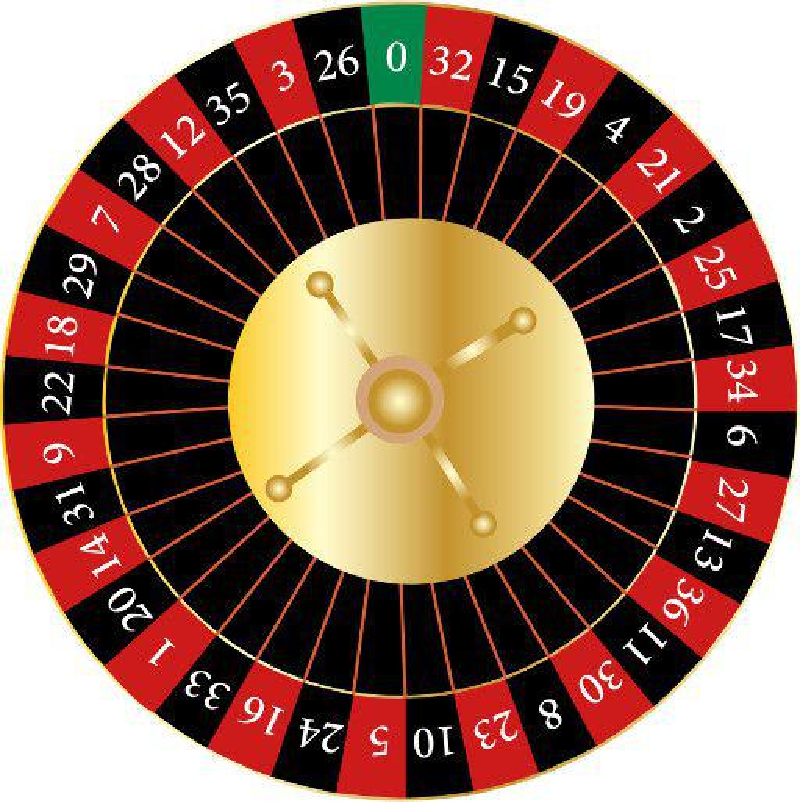
\includegraphics[width=0.75\textwidth]{figs/roulette.pdf}
\end{minipage}%
\begin{minipage}{0.5\textwidth}
  The standard European roulette wheel shown to the left (\href{https://www.vecteezy.com/vector-art/658761-casino-roulette-wheel}{source}) has 37 pockets labelled ``0'' through ``36''.
  18 of these pockets are coloured red, 18 are coloured black and 1 (pocket ``0'') is coloured green.
\end{minipage}

\noindent What is the outcome space $A$ for a spin of the roulette wheel?
With $\cF = A$, what are the probabilities $p_{\al}$ for a fair wheel?
With
\begin{equation*}
  \cF = \left\{\mbox{ball in a red pocket, ball in a black pocket, ball in the green pocket}\right\},
\end{equation*}
what are the corresponding probabilities $p_{\text{red}}$, $p_{\text{black}}$ and $p_{\text{green}}$?
\begin{mdframed}
  \ \\[100 pt]
\end{mdframed}

We conclude this section with two \textbf{comments} on the process of assigning probabilities to events (which is called \textit{modelling}): \\[-24 pt]
\begin{itemize}
  \item We saw above that \textit{symmetries} are a powerful way to constrain probabilities.
        The symmetry between the six sides of a fair die, the two sides of a fair coin, and the 37 pockets of a fair roulette wheel each sufficed to completely fix the corresponding probabilities $p_{\al}$.
  \item Modelling can also be guided by empirical information obtained by repeating an experiment many times.
        For example, if we don't know whether a set of dice are fair, we will be able to infer their probabilities $p_{\al}$ (with a certain confidence level) by rolling them enough times.
        The need to repeat the experiment many times comes from the law of large numbers, to which we now turn.
\end{itemize}
% ------------------------------------------------------------------



% ------------------------------------------------------------------
\subsection{Law of large numbers}
Let's continue considering the setup introduced above, with
\begin{equation}
  \label{eq:finite_set}
  \cF = A = \left\{X_1, X_2, \cdots, X_n\right\}
\end{equation}
for finite $n$, and probabilities $p_{\al} = P(X_{\al})$ that obey
\begin{align*}
  p_{\al} & \in [0, 1] &
  \sum_{\al = 1}^n p_{\al} & = 1.
\end{align*}
We can generalize this notation by writing instead
\begin{equation*}
  \sum_{X \in A} P(X) = 1,
\end{equation*}
which provides simple expressions for the \textbf{mean} $\mu$ and \textbf{variance} $\si^2$ of the probability space,
\begin{align}
              \mu = \vev{X} = & \sum_{X \in A} X P(X)            \label{eq:mean} \\
  \si^2 = \vev{(X - \mu)^2} = & \sum_{X \in A} (X - \mu)^2 P(X). \label{eq:var}
\end{align}
The angle bracket notation indicates the \textbf{expected} (or \textbf{expectation}) \textbf{value} with general definition
\begin{equation}
  \label{eq:expect_disc}
  \vev{f(X)} = \sum_{X \in A} f(X) P(X),
\end{equation}
which is a linear operation,
\begin{equation*}
  \vev{c\cdot f(X) + g(X)} = c\vev{f(X)} + \vev{g(X)}.
\end{equation*}
\newpage % WARNING: FORMATTING BY HAND
\noindent The square root of the variance, $\sqrt{\si^2} = \si$, is the \textbf{standard deviation}.
What is \si expressed in terms of $\vev{X^2}$ and $\vev{X}^2$?
\begin{mdframed}
  \ \\[100 pt]
\end{mdframed}

We now define a new experiment that consists of \textit{repeating} the original experiment $R$ times, with each repetition independent of all the others.
Using the same measurement as before for each repetition, we obtain a new outcome space that we can call $B$.
For $R = 4$, what are some representative outcomes in the set $B$?
What is the total size of $B$?
\begin{mdframed}
  \ \\[100 pt]
\end{mdframed}

Each outcome in $B$ contains $R$ different $X^{(r)} \in A$ (with $\vev{X^{(r)}} = \mu$ and $\vev{(X^{(r)} - \mu)^2} = \si^2$), one for each repetition $r = 1, \cdots, R$.
Considering the case $R = 4$ for simplicity, any element of $B$ can be written as $X_i^{(1)} X_j^{(2)} X_k^{(3)} X_l^{(4)} \in B$ with corresponding probability
\begin{equation*}
  P_B\left(X_i^{(1)} X_j^{(2)} X_k^{(3)} X_l^{(4)}\right) = P_A\left(X_i^{(1)}\right) P_A\left(X_j^{(2)}\right) P_A\left(X_k^{(3)}\right) P_A\left(X_l^{(4)}\right),
\end{equation*}
using subscripts to distinguish between the single-experiment ($A$) and repeated-experiment ($B$) probability spaces.

Averaging over all $R$ repetitions defines the \textit{arithmetic mean}
\begin{equation*}
  \Xbar_R = \frac{1}{R} \sum_{r = 1}^R X^{(r)}.
\end{equation*}
Unlike the true mean $\mu$, the arithmetic mean $\Xbar_R$ is a random variable---a number that may be different for each element of $B$.
That said, $\Xbar_R$ and $\mu$ are certainly related, and so long as the standard deviation exists (i.e., $\si^2$ is finite), this relation can be proved rigorously in the limit $R \to \infty$.\footnote{In the computer-based project we will numerically investigate a case with divergent $\si^2$.}

Here we will not be fully rigorous, and take it for granted that
\begin{equation*}
  \vev{\left(X^{(i)} - \mu\right)\left(X^{(j)} - \mu\right)} = \si^2 \de_{ij} = \left\{\begin{array}{ll}\si^2 & \mbox{for } i = j \\ 0 & \mbox{for } i \ne j\end{array}\right.,
\end{equation*}
where the \textit{Kronecker delta} $\de_{ij} = 1$ for $i = j$ and vanishes for $i \ne j$.
This is a consequence of the assumed independence of the different repetitions.
Using this result and the relation $\big(\sum_i a_i\big)\big(\sum_j b_j\big) = \sum_{i, j} \left(a_i b_j\right)$, express the following quantity in terms of \si and $R$:
\begin{mdframed}
  $\displaystyle \vev{\left(\frac{1}{R} \sum_{r = 1}^R X^{(r)} - \mu\right)^2} = $ \\[100 pt]
\end{mdframed}
You should find that your result vanishes in the limit $R \to \infty$, so long as $\si^2$ is finite.
Since the square makes this expectation value a sum of non-negative terms, it can vanish only if every one of those terms is individually zero.

\begin{shaded}
  This result establishes the \textbf{law of large numbers}:
  \begin{equation}
    \lim_{R \to \infty} \frac{1}{R} \sum_{r = 1}^R X^{(r)} = \mu,
  \end{equation}
  where we have assumed $\vev{X^{(r)}} = \mu$ and $\vev{(X^{(r)} - \mu)^2} = \si^2$ are finite.
\end{shaded}
% ------------------------------------------------------------------



% ------------------------------------------------------------------
\subsection{Probability distributions}
It is not necessary to make the assumption (\eq{eq:finite_set}) that we are dealing with a countable number of $X_1, \cdots, X_n$.
The considerations above continue to hold even if the random variable $X$ is a continuous real number.
In this case, however, the identification of probabilities with outcomes $X$ is slightly more complicated, which will be relevant when we consider the central limit theorem in the next section.

When the outcome can be any number on the real line, the fundamental object is a \textbf{probability distribution} (or \textbf{density function}) $p(x)$ defined for all $x \in \Rbb$.
Starting from this density, a probability is determined by integrating over a given interval.
Calling this interval $[a, b]$, the integration produces the probability that the outcome $X$ lies within the interval,
\begin{equation*}
  P\left(a \leq X \leq b\right) = \int_a^b p(x) dx.
\end{equation*}

We similarly generalize the definition of an expectation value (\eq{eq:expect_disc}) to an integral over the entire domain of the  probability distribution,
\begin{equation*}
  \vev{f(x)} = \int f(x) \; p(x) \; dx.
\end{equation*}
We will omit the limits on integrals over the entire domain, so for $x \in \Rbb$ we implicitly have $\int dx = \int_{-\infty}^{\infty} dx$.
An important set of expectation values is
\begin{equation}
  \label{eq:expect_cont}
  \vev{x^{\ell}} = \int x^{\ell} \; p(x) \; dx,
\end{equation}
which provide the mean and variance of the probability distribution $p(x)$, through generalizations of Eqs.~\ref{eq:mean}--\ref{eq:var}:
\begin{align}
  \label{eq:mean_var}
  \mu   & = \vev{x} = \int x \; p(x) \; dx&
  \si^2 & = \vev{x^2} - \vev{x}^2.
\end{align}
The expression for the variance should be familiar from your determination of the standard deviation in an earlier gap.
Unless stated otherwise, we will assume the mean and variance are both finite for the probability distributions we consider.
% ------------------------------------------------------------------



% ------------------------------------------------------------------
\subsection{Central limit theorem}
The central limit theorem is a major result of probability theory.
Over the years it has been phrased in many equivalent ways, and many distinct variants of the theorem exist to accommodate different conditions and assumptions.
\TODO{...}
% ------------------------------------------------------------------


\newpage
% ------------------------------------------------------------------
\renewcommand{\thisweek}{MATH327 Week 2}
\renewcommand{\moddate}{Last modified 7 Feb.~2021}
\setcounter{section}{2}
\setcounter{subsection}{0}
\phantomsection
\addcontentsline{toc}{section}{Week 2: Micro-canonical ensemble}
\section*{Week 2: Micro-canonical ensemble}

\subsection{Statistical ensembles and thermodynamic equilibrium}
We begin this week by developing the concept of \textit{statistical ensembles} (introduced by \href{https://en.wikipedia.org/wiki/Josiah_Willard_Gibbs}{J.\ Willard Gibbs} in the early 1900s), building on the probability foundations we laid last week.
As forecast last week, we will be interested in `experiments' that simply allow a collection of degrees of freedom to evolve in time, subject to certain constraints.
At a given time $t_1$, the disposition of these degrees of freedom defines the state $\om_1$ of the system.
To consider a couple of examples, what would be a representative state for a system of $8$ \textit{spins} (arrows that can point either `up' or `down') arranged in a line?\footnote{We will consider \href{https://en.wikipedia.org/wiki/Spin_model}{spin systems} extensively in this module.  In addition to obeying simple mathematics analogous to flipping coins, spins also serve as good models of physical systems such as magnetic molecules.}
What information would characterize the state of $N$ hydrogen (H$_2$) molecules in a container?
\begin{mdframed}
  \ \\[100 pt]
\end{mdframed}

At a different time $t_2$, the system's state $\om_2$ is generally different from $\om_1$.
However, there are some measurements we can perform on these states that always produce the same outcome as the system evolves in time.
These measurements define \textit{conserved quantities}, an important example of which is the total energy $E$ \textit{inside} an isolated (or `closed') system,
\begin{equation*}
  E(\om_1) = E(\om_2).
\end{equation*}
The conservation of energy is presumably a familiar concept, and you may also know that it can be rigorously proven through \href{https://en.wikipedia.org/wiki/Emmy_Noether}{Emmy Noether}'s theorem.\footnote{This proof holds only in `flat' space-time as opposed to the curved space-time manifolds than arise in general relativity---which is far beyond the scope of this module.}
Because statistical physics was first developed when conservation of energy was primarily an empirical observation rather than a proven result, it was given a more grandiose name: the \textbf{first law of thermodynamics}.
Another way of stating the first law is that any change in the internal energy of one particular system \Om must be matched by an equal and opposite change in the energy of some other system(s) with which \Om is in contact.
We will return to this formulation of the first law in future weeks.

For now, let's return to the \textbf{examples} above, and suppose that the spin system is placed in an external magnetic field.
If a spin is parallel to the field, it contributes energy $-H$ to the total energy $E$ of the system.
If a spin is anti-parallel to the field, it instead contributes energy $H > 0$.
What is the total energy $E$ of a system of $N$ spins in a state with $n_+$ spins anti-parallel to the field and $n_- = N - n_+$ parallel to it?
What is $E$ for the representative $N = 8$-spin state you wrote down above?
How many of the $2^8 = 256$ states of the spin system have this energy?
\begin{mdframed}
  \ \\[100 pt]
\end{mdframed}
For the $N$ hydrogen molecules in a container, we can write a simple expression for the energy $E$ by treating each molecule as a \textit{point-like particle}, with no size or structure.
In this case each molecule contributes only its kinetic energy to $E$,
\begin{equation*}
  E = \frac{m}{2} \sum_{i = 1}^N \vec{v}_i^{\,2} = \frac{1}{2m} \sum_{i = 1}^N \vec{p}_i^{\,2},
\end{equation*}
where $\vec v_i$ is the velocity of the $i$th molecule, $\vec p_i = m \vec v_i$ is its momentum, and all molecules have exactly the same mass $m$.

As emphasized in last week's introduction, we treat the time evolution of the system as a stochastic process in which the system probabilistically adopts a sequence of states $\om_i \in \Om$:
\begin{equation*}
  \om_1 \lra \om_2 \lra \om_3 \lra \om_4 \lra \cdots
\end{equation*}
This attitude is adopted as a matter of practicality rather than one of principle.
In principle, Newton's laws would allow us to exactly predict the time evolution of (say) $\sim$$10^{23}$ hydrogen molecules, but only by specifying $\sim$$10^{23}$ initial conditions and solving $\sim$$10^{23}$ differential equations.
Since we cannot hope to write down so much information or carry out so many computations, we instead apply probability theory in order to analyze these systems.

\begin{shaded}
  This leads us to the following core definition: A \textbf{statistical ensemble} is the set of all states $\Om = \left\{\om_1, \om_2, \cdots\right\}$ that a system can possibly adopt through its time evolution.
  Each state $\om_i$ has some probability $p_i$ of being adopted by the system, so we can recognize a statistical ensemble as a probability space.
\end{shaded}

Because these states $\om_i$ depend on the `microscopic' degrees of freedom that compose the overall system, we will refer to them as \textbf{micro-states} from now on.
From last week's definition of probability, we have the requirement $\sum_i p_i = 1$, which simply means that the system must be in \textit{some} micro-state at any point in time.
The fact that time evolution cannot change any conserved quantities, as discussed above, means that such conserved quantities characterize statistical ensembles.
We will define different types of statistical ensemble that depend on the specific set of conserved quantities.

\begin{shaded}
  This week we define a \textbf{micro-canonical ensemble} to be a statistical ensemble characterized by conserved internal energy $E$ and conserved number of degrees of freedom $N$ (which we will call \textbf{particle number} for short).
\end{shaded}

According to the discussion above, this means that a system governed by the micro-canonical ensemble is \textit{isolated} in the sense that it cannot exchange energy or particles with any other system.

Now that the micro-canonical ensemble is defined, we can connect it to our intuition from everyday physical systems.
Let's consider a collection of particles moving around and bouncing (or `\textit{scattering}') off each other in a sealed container.
To a first approximation, this should describe the behaviour of air in a room, which our lived experience indicates is spread quite uniformly throughout the room in a way that is stable as time passes.
We do not expect all the air in a room to be concentrated in any one corner, nor do we expect strong collective gusts of wind without some clear external influence.

These qualitative expectations illustrate the idea of \textbf{thermodynamic equilibrium}, an axiomatic concept in statistical physics.\footnote{Our expectation that physical systems generically evolve towards thermodynamic equilibrium as time passes is more formally expressed as the \href{https://en.wikipedia.org/wiki/Ergodic_hypothesis}{ergodic hypothesis}.}
We can mathematically define thermodynamic equilibrium through the probabilities $p_i$ that appear in the micro-canonical ensemble.

\begin{shaded}
  A micro-canonical system \Om with $M$ micro-states $\om_i$ is in thermodynamic equilibrium if and only if all probabilities $p_i$ are equal.
  If $M$ is finite, the requirement $\sum_i p_i = 1$ implies
  \begin{equation}
    \label{eq:micro_equil}
    p_i = \frac{1}{M}.
  \end{equation}
\end{shaded}

The full meaning and significance of this definition are not immediately obvious, and we will continue exploring them through consideration of derived quantities such as entropy and temperature.
First, we emphasize that this equilibrium is indeed \textit{dynamic}: There is not a single `equilibrium state' that the system approaches; instead, the system continues probabilistically adopting different states as it evolves in time.
% ------------------------------------------------------------------



% ------------------------------------------------------------------
\subsection{Entropy and its properties}
\subsubsection{Definition of entropy}
We can gain further insight into thermodynamic equilibrium by considering a famous derived quantity.
\begin{shaded}
  The \textbf{entropy} of a statistical ensemble \Om with a countable number of micro-states $M$ is defined to be
  \begin{equation}
    \label{eq:entropy}
    S = - \sum_{i = 1}^M p_i \log p_i,
  \end{equation}
  where $p_i$ is the probability for micro-state $\om_i$ to occur.
  Unless otherwise specified, ``$\log$'' indicates the natural logarithm of base $e$.
\end{shaded}

When the system under consideration is in thermodynamic equilibrium, we expect derived quantities such as the entropy to be stable over time, even as different micro-states are probabilistically adopted.
This implies that such derived quantities are functions of the conserved quantities that are the same for all micro-states.
Therefore, for the micro-canonical ensemble, the equilibrium entropy $S(E, N)$ would be a function of the conserved energy and particle number.

By inserting \eq{eq:micro_equil} into \eq{eq:entropy} you can quickly compute a simple expression for the entropy of a micro-canonical ensemble in thermodynamic equilibrium:
\begin{mdframed}
  \ \\[50 pt]
\end{mdframed}
%\begin{equation}
%  \label{eq:}
%  S = - \sum_{i = 1}^M \frac{1}{M} \log \left(\frac{1}{M}\right) = \log M.
%\end{equation}
Your result should depend only on the number of micro-states $M$, and diverge as $M \to \infty$.
While the energy $E$ and particle number $N$ are not explicit in this expression, $\left\{E, N, M\right\}$ are inter-related and might be expressed in terms of each other depending on the particular situation under consideration.
For example, what is the equilibrium entropy of the system of $N$ spins considered above, if the external magnetic field is turned off (so $H = 0$ implying $E = 0$)?
\begin{mdframed}
  \ \\[100 pt]
\end{mdframed}
% ------------------------------------------------------------------



% ------------------------------------------------------------------
\subsubsection{Extensivity}
The increase in entropy for an increasing number of micro-states $M$ is a reflection of entropy being an \textit{extensive} quantity. % TODO: as opposed to intrinsic temperature
Extensive quantities are formally defined by considering how they behave if two isolated systems are \textit{analyzed} as a single system---while still remaining isolated from each other, exchanging neither energy nor particles.
This is clearest to consider through the specific example shown below of two isolated spin systems, $\Om_1$ \& $\Om_2$, respectively characterized by the corresponding energies $E_1$ \& $E_2$ and particle numbers $N_1$ \& $N_2$.
To simplify the subsequent analysis, we can assume that both systems are placed in external magnetic fields with the same $H$, so that $E_S = H\left(n_+^{(S)} - n_-^{(S)}\right)$ for $S = 1$, $2$.
\begin{center}
  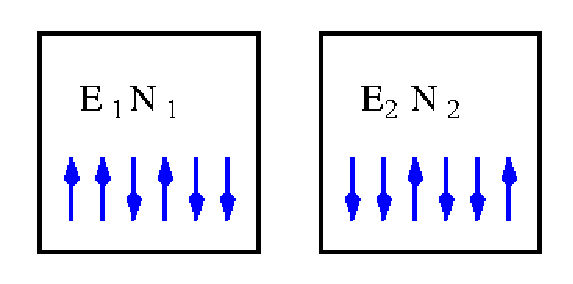
\includegraphics[width=0.7\textwidth]{figs/week02_entropy-separate.pdf}
\end{center}

In the figure above, we can take system $\Om_1$ to have $M_1$ micro-states with probabilities $p_i$ while system $\Om_2$ has $M_2$ micro-states with probabilities $q_k$.
(As discussed above, $M_S$ is a function of $E_S$ and $N_S$ for $S = 1$, $2$.)
Then, even without assuming thermodynamic equilibrium, the entropies of the two systems are
\begin{align*}
  S_1 & = - \sum_{i = 1}^{M_1} p_i \log p_i &
  S_2 & = - \sum_{k = 1}^{M_2} q_k \log q_k.
\end{align*}

\begin{center}
  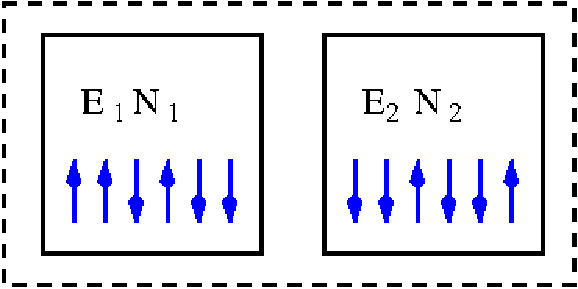
\includegraphics[width=0.7\textwidth]{figs/week02_entropy-combo.pdf}
\end{center}

Now we keep these two (sub)systems isolated from each other, but consider them as a combined system $\Om_{1+2}$, as illustrated above.
In order to compute the entropy $S_{1+2}$, we first need to figure out how many micro-states the combined system could possibly adopt ($M_{1+2}$), and then determine the corresponding probability for each micro-state.
Both steps are simplified by the systems being isolated from each other, so that they are statistically independent.
Specifically, with subsystem $\Om_1$ in a fixed micro-state $\om_i^{(1)}$, subsystem $\Om_2$ could independently inhabit any of its $M_2$ micro-states.
What is the resulting $M_{1+2}$ in terms of $M_1$ and $M_2$?
\begin{mdframed}
  $M_{1+2} = $ \\[50 pt]
\end{mdframed}
Similarly, statistical independence means that the combined probability of subsystem $\Om_1$ adopting micro-state $\om_i^{(1)}$ while subsystem $\Om_2$ adopts $\om_k^{(2)}$ is the product of the individual probabilities, $p_i q_k$.
We can check that this is a well-defined probability, with
\begin{equation*}
  \sum_{M_{1+2}} p_i q_k = \sum_{i = 1}^{M_1} \sum_{k = 1}^{M_2} p_i q_k = \left[\sum_{i = 1}^{M_1} p_i\right]\cdot \left[\sum_{k = 1}^{M_2} q_k\right] = 1\cdot 1 = 1.
\end{equation*}
Inserting the probability $p_i q_k$ into \eq{eq:entropy}, and recalling $\log(a\cdot b) = \log a + \log b$, what is the combined entropy $S_{1+2}$ of these two independent subsystems?
\begin{mdframed}
  $S_{1+2} = $ \\[100 pt]
\end{mdframed}
You should find that the entropies of the two isolated subsystems add up to form the total, which is also the case for the energies and particle numbers,
\begin{align*}
  E_{1+2} & = E_1 + E_2 &
  N_{1+2} & = N_1 + N_2 &
  S_{1+2} & = S_1 + S_2
\end{align*}

\begin{shaded}
  \textbf{Extensive} quantities are \href{https://goldbook.iupac.org/terms/view/E02281}{defined} to be those that add up across independent subsystems.
  Examples include the energy, particle number and entropy as shown above.
  This can be contrasted with \textbf{intensive} quantities, which are \href{https://goldbook.iupac.org/terms/view/I03074}{defined} to be independent of the extent of the system (and hence the same for subsystems as for the combined system).
  We will see an example of this next week. % External magnetic field strength $H$ is control parameter rather than system property...
  It is possible for quantities to be neither extensive nor intensive.
\end{shaded}

Finally, if we were to assume that each subsystem is (independently) in thermodynamic equilibrium, with finite $M_1$ and $M_2$,
\begin{align*}
  p_i & = \frac{1}{M_1} & q_k & = \frac{1}{M_2} \\
  S_1 & = \log M_1      & S_2 & = \log M_2.
\end{align*}
then we would find as a consequence that their combination is also in thermodynamic equilibrium, since
\begin{equation*}
  p_i q_k = \frac{1}{M_1 M_2} = \frac{1}{M_{1+2}}
\end{equation*}
is the same for every combined micro-state.
% ------------------------------------------------------------------



% ------------------------------------------------------------------
\subsubsection{Second law of thermodynamics}
Let's continue considering the two spin (sub)systems discussed above, with one significant change: We suppose the two subsystems are now able to exchange energy (but not particles) with each other.
We'll say they are in \textit{thermal contact} with each other, rather than being fully isolated.
This is illustrated by the figure below:
\begin{center}
  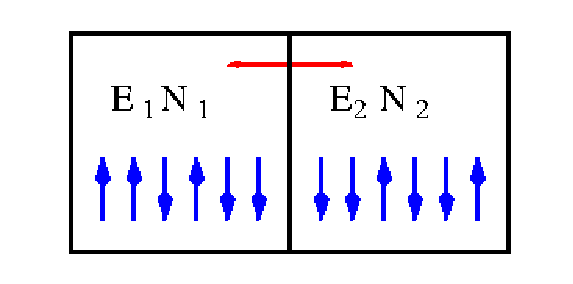
\includegraphics[width=0.7\textwidth]{figs/week02_entropy-exchange.pdf}
\end{center}
The total energy $E = E_1 + E_2$ remains conserved, so the overall system \Om is still governed by the micro-canonical ensemble.
However, the individual energies $E_1$ and $E_2$ can now change as time passes, meaning that \textit{each subsystem is no longer micro-canonical}.

The overall \Om is \textit{not} the same as the combined $\Om_{1+2}$ considered above.
We need to reconsider the total number of micro-states $M$ that \Om could adopt, which is much more difficult than before because we can no longer apply statistical independence.
Our main remaining tool is the conservation of the total energy $E$.

Considering a micro-state in which the $N_1$ spins contribute energy $e_1$ to the total, we know that the $N_2$ spins must contribute the remaining $e_2 = E - e_1$.
Our work above implies there are $M_{e_1} = M_{e_1}^{(1)} M_{E - e_1}^{(2)}$ micro-states providing this particular distribution of energies, where $M_{e_1}^{(1)}$ is the number of micro-states of the formerly isolated subsystem $\Om_1$ with energy $e_1$, and $M_{E - e_1}^{(2)}$ similarly corresponds to $\Om_2$ with energy $E - e_1$.
We also know that it's possible to have $e_1 = E_1$, since that's the initial energy of $\Om_1$ before it was brought into thermal contact with $\Om_2$.
When $e_1 = E_1$, we have $M_{e_1} = M_1 M_2$, covering all the micro-states of the combined system when the two subsystems were isolated.
\textit{In addition}, we also have to count any other microstates for which $e_1 \ne E_1$:
\begin{equation*}
  M = \sum_{e_1} M_{e_1}^{(1)} M_{E - e_1}^{(2)} = M_1 M_2 + \sum_{e_1 \ne E_1} M_{e_1}^{(1)} M_{E - e_1}^{(2)} \geq M_1 M_2.
\end{equation*}
(It could be that $e_1 = E_1$ is the only possibility.)
This is all we can say without specifying more details of a particular example, but it allows us to obtain a famous result for the total entropy $S$ of \Om \textit{in thermodynamic equilibrium}:
\begin{mdframed}
  $S = \log M \geq $ \\[100 pt]
\end{mdframed}

\begin{shaded}
  You have now derived a form of the \textbf{second law of thermodynamics},
  \begin{equation*}
    S \geq S_{1 + 2} = S_1 + S_2.
  \end{equation*}
  In words, whenever isolated (sub)systems in thermodynamic equilibrium are brought into thermal contact with each other and allowed to exchange energy, the total entropy of the overall system can never decrease.
\end{shaded}

This has many far-reaching consequences, the first of which is a more general definition of thermodynamic equilibrium that (unlike \eq{eq:micro_equil}) will also apply when we consider statistical ensembles other than the micro-canonical ensemble.
For simplicity we assume that any system under consideration has a finite number of micro-states, which means that its entropy is bounded from above.
To motivate the definition below, note that the overall system \Om may have undergone an equilibration process to reach its thermodynamic equilibrium after its two (independently equilibrated) subsystems were brought into thermal contact---and in this process the entropy was non-decreasing.

\begin{shaded}
  A system is defined to be in \textbf{thermodynamic equilibrium} if its entropy is maximal.
\end{shaded}

We can \textit{derive} \eq{eq:micro_equil} from this definition.
All we need to do is maximize the entropy $S = - \sum_i p_i \log p_i$ subject (for the micro-canonical ensemble) to the three constraints of conserved energy, conserved particle number, and well-defined probabilities $\sum_i p_i = 1$.
Only the last will turn out to matter, and can be incorporated into the maximization through the method of \textbf{Lagrange multipliers}.
In case you are not familiar with this method, it involves maximizing the modified entropy
\begin{equation*}
  \Sbar = S + \la\left(\sum_{i = 1}^M p_i - 1\right) = - \sum_{i = 1}^M p_i \log p_i + \la\left(\sum_{i = 1}^M p_i - 1\right),
\end{equation*}
where the parameter \la is called the `multiplier'.
In short, this procedure is valid because $\displaystyle \pderiv{\Sbar}{\la} = 0$, so that any extremum of \Sbar corresponds to an extremum of $S$ when the multiplier is set to $\la = 0$.
Recalling $\displaystyle \pderiv{}{x_k} \sum_i f(x_i) = \pderiv{f(x_k)}{x_k}$, what is the probability $p_k$ that maximizes $\Sbar$?
\begin{mdframed}
  $\displaystyle 0 = \pderiv{\Sbar}{p_k} = $ \\[100 pt]
\end{mdframed}
You should find that $p_k$ is some constant that depends on $\la$.
We don't care about $\la$; so long as we know $p_k$ is constant, then $p_k = \frac{1}{M}$ to satisfy $\sum_k p_k = 1$.
As advertised, we recover \eq{eq:micro_equil} from our new definition of thermodynamic equilibrium based on the second law.
% ------------------------------------------------------------------



% ------------------------------------------------------------------
\subsection{Temperature}
In the micro-canonical ensemble, the conserved internal energy and particle number are fundamental, while the temperature (like the entropy) is a derived quantity.
As discussed below \eq{eq:entropy}, in thermodynamic equilibrium such derived quantities are functions of the conserved $\left\{E, N\right\}$.
Here we will simply state the definition of temperature for the micro-canonical ensemble, and then check that our definition reproduces our expectations from everyday experiences.

\begin{shaded}
  In thermodynamic equilibrium, the \textbf{temperature} in the micro-canonical ensemble is defined by
  \begin{equation}
    \label{eq:temperature}
    \frac{1}{T(E)} = \left. \pderiv{S}{E}\right|_N.
  \end{equation}
  In words, the (inverse) temperature is set by the dependence of the entropy on the internal energy for a fixed number of degrees of freedom.
\end{shaded}

Since this definition is not terribly intuitive, we will again gain insight by working through the \textbf{example} of $N$ spins in a line, in an external magnetic field of strength $H$.
We saw above that $E = H(n_+ - n_-)$ for $n_+$ and $n_- = N - n_+$ spins respectively aligned anti-parallel and parallel to the magnetic field.
Each (conserved) value of $E$ defines a \textit{different} micro-canonical system, which we can expect to have a different number of micro-states $M(E)$, different entropy $S(E)$ and different temperature $T(E)$.
We will compute the functional forms of each of these three quantities, starting with $M(E)$.

Even though the total energy $E$ remains fixed as time passes, individual spins can `flip' between pointing parallel or anti-parallel to the magnetic field.
Such spin flips simply have to come in pairs so that the overall $n_{\pm}$ both remain the same.
As illustration, what are the spin configurations that produce the minimal energy $E_{\text{min}} \equiv E_0$ and the next-to-minimal $E_1$?
What are $E_0$ and $E_1$ in terms of $\left\{N, H\right\}$, and how many distinct micro-states are there for each of $E_0$ and $E_1$?
\begin{mdframed}
  \ \\[100 pt]
\end{mdframed}
Your results should generalize to
\begin{equation*}
  M(E_{n_+}) = \binom{N}{n_+} = \frac{N!}{n_+! \; (N - n_+)!}.
\end{equation*}

To take the derivative in \eq{eq:temperature}, we need to express $n_+$ in terms of $\left\{E, N\right\}$.
For this it is convenient to define $\nu = E / H$.
\begin{mdframed}
  \ \\[100 pt]
\end{mdframed}

\TODO{Being written...}
% ------------------------------------------------------------------



% ------------------------------------------------------------------
\newpage % TODO: Placeholder...
\subsection{Heat exchange}
\TODO{Being written...}
% ------------------------------------------------------------------


\newpage
% ------------------------------------------------------------------
\renewcommand{\thisweek}{MATH327 Week 3}
\renewcommand{\moddate}{Last modified 4 Mar.~2021}
\setcounter{section}{3}
\setcounter{subsection}{0}
\phantomsection
\addcontentsline{toc}{section}{Week 3: Canonical ensemble}
\section*{Week 3: Canonical ensemble}
\subsection{\label{sec:reservoir}The thermal reservoir}
\subsubsection{\label{sec:replicas}Replicas and occupation numbers}
While it is relatively easy to prevent particle exchange, for example by sealing gases inside airtight containers, it is not practical to forbid energy exchange as would be needed to fully isolate statistical systems.
Any thermal insulator is imperfect, and even in the deepest reaches of space we would still be bombarded by cosmic microwave radiation.
In practice it is more convenient to work with physical systems that are characterized by their (intensive) temperatures rather than their (extensive) internal energies.

\begin{shaded}
  This leads us to define a \textbf{canonical ensemble} to be a statistical ensemble characterized by its fixed temperature $T$ and conserved particle number $N$, with the temperature held fixed through contact with a \textbf{thermal reservoir}.
\end{shaded}

The second part of this definition connects the fixed temperature to the fundamental fact of energy conservation (the first law of thermodynamics).
This is done by proposing that our system of interest \Om is in thermal contact with a much larger external system $\Om_{\text{res}}$---the thermal reservoir, sometimes called a ``heat bath''.
The overall combined system $\Om_{\text{tot}} = \Om_{\text{res}} \otimes \Om$ is governed by the micro-canonical ensemble, with conserved total energy $E_{\text{tot}} = E_{\text{res}} + E \approx E_{\text{res}}$, while the energy $E$ of \Om is allowed to fluctuate.
The key qualitative idea is that, in thermodynamic equilibrium, \Om has a negligible effect on the overall system.
In particular, the temperature of that overall system---and therefore the temperature of $\Om$, by intensivity---is set by the reservoir and remains fixed even as $E$ fluctuates.
This effectively generalizes the setup we used to analyze heat exchange last week, where we saw that thermal contact causes a net flow of energy from hotter systems to colder systems, cooling the former by heating the latter.

The mathematical realization of this argument, as developed by J.\ Willard Gibbs, proceeds by considering a well-motivated ansatz for the form of the thermal reservoir $\Om_{\text{res}}$.
\textcolor{green}{The goal}, which will be useful to keep in mind as we go through the lengthy analysis, is to show that the specific form of $\Om_{\text{res}}$ is ultimately irrelevant.
This will allow us to work directly with the system of interest, $\Om$, independent of the details of the thermal reservoir that fixes its temperature.

Without further ado, we take $\Om_{\text{tot}}$ to consist of many ($R \gg 1$) identical \textbf{replicas} of the system \Om that we're interested in.
All of these replicas are in thermal contact with each other, and in thermodynamic equilibrium.\footnote{The thermal contact between any two replicas can be indirect, mediated by a sequence of intermediate replicas.  This transitivity of thermodynamic equilibrium is sometimes called the \href{https://en.wikipedia.org/wiki/Zeroth_law_of_thermodynamics}{zeroth law of thermodynamics}.  It declares that if systems $\Om_A$ \& $\Om_B$ are in thermodynamic equilibrium while systems $\Om_B$ \& $\Om_C$ are in thermodynamic equilibrium, then $\Om_A$ \& $\Om_C$ must also be in thermodynamic equilibrium.}
Choosing one of the replicas to be the system of interest, $\Om$, the other $R - 1 \gg 1$ replicas provide the thermal reservoir $\Om_{\text{res}}$.
Assuming we want to study reasonable systems $\Om$, this ansatz ensures that $\Om_{\text{res}}$ is also reasonable, simply much larger.

An extremely small example of this setup is illustrated by the figures below, where the system of interest consists of only $N = 2$ spins.
For now we assume the spins are \textit{distinguishable}, so that $\downarrow\uparrow$ and $\uparrow\downarrow$ are both distinct micro-states.
This means that each individual replica has only the $M = 4$ micro-states $\om_i$ defined below.
\begin{center}
  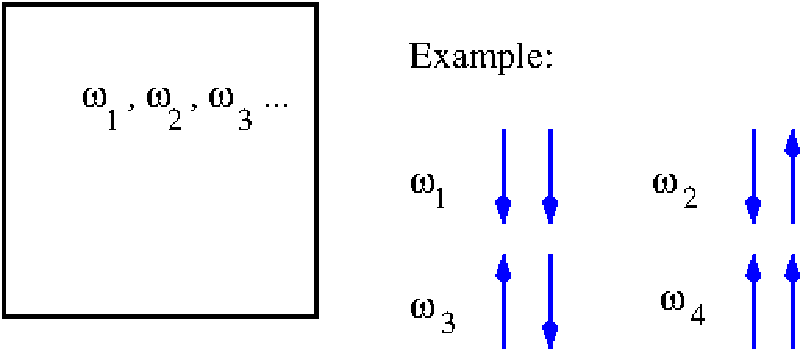
\includegraphics[width=0.7\textwidth]{figs/week03_spin-system.pdf}
\end{center}
To form the overall system $\Om_{\text{tot}}$ we now bring together the $R = 9$ replicas shown below.
We draw boxes around each replica to remind us that they are allowed to exchange only energy with each other, while the $N = 2$ spins are conserved in each replica.
We pick out one of these replicas (coloured red) to serve as the system \Om we will consider.
The other $8$ are the thermal reservoir $\Om_{\text{res}}$ that fixes the temperature of $\Om$.
\begin{center}
  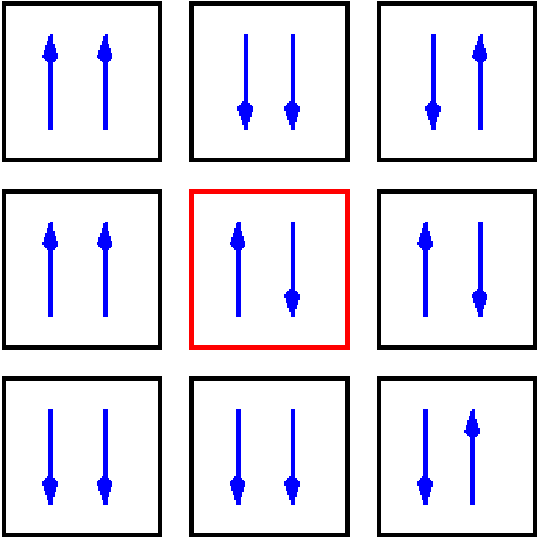
\includegraphics[width=0.7\textwidth]{figs/week03_spin-reservoir.pdf}
\end{center}

A convenient way to analyze the overall system of $R$ replicas, $\Om_{\text{tot}}$, is to define the \textbf{occupation number} $n_i$ to be the number of replicas that adopt the micro-state $\om_i \in \Om$ in any given micro-state of $\Om_{\text{tot}}$.
The index $i \in \left\{1, 2, \cdots, M\right\}$ runs over all $M$ micro-states of $\Om$.
In the example above, three of the replicas in the second figure have the micro-state $\om_1 = \downarrow\downarrow$, meaning $n_1 = 3$.
What are the occupation numbers $\left\{n_2, n_3, n_4\right\}$ for the other three $\om_i$ in the figures above?
Are all replicas are accounted for, $\sum_i n_i = R$?
\begin{mdframed}
  \ \\[50 pt]
\end{mdframed}
Normalizing the occupation number by $R$ gives us a well-defined \textit{occupation probability}, $p_i = n_i / R$ with $\sum_i p_i = 1$.
This $p_i$ is the probability that if we choose a replica at random it will be in micro-state $\om_i$.

Now let us consider conservation of energy, which continues to apply to the total energy $E_{\text{tot}}$ of the overall system $\Om_{\text{tot}}$.
We assume that each replica's energy $E_r$ is independent of all the other replicas.
This is guaranteed for the non-interacting systems we will focus on until week $10$, and also holds when interactions are allowed within each replica but not between different replicas.
The thermal contact between replicas allows $E_r$ to fluctuate (subject to conservation of $E_{\text{tot}}$), but there are only $M$ possible values $E_i$ it can have, corresponding to the $M$ micro-states $\om_i \in \Om$.
This allows us to rearrange a sum over replicas into a sum over the micro-states of $\Om$:
\begin{equation}
  \label{eq:canon_Etot}
  E_{\text{tot}} = \sum_{r = 1}^R E_r = \sum_{i = 1}^M n_i E_i,
\end{equation}
with the occupation number $n_i$ counting how many times micro-state $\om_i$ appears among the $R$ replicas.
We can assume that $R$ and $M$ are both finite, so we don't need to worry about rearranging infinite sums.
% ------------------------------------------------------------------



% ------------------------------------------------------------------
\subsubsection{\label{sec:canon_part}Partition function}
Following Gibbs, we have already taken the thermal reservoir $\Om_{\text{res}}$ to consist of $R - 1$ replicas of the system of interest, $\Om$.
The next step is to further simplify the mathematics by assuming that the overall $R$-replica system $\Om_{\text{tot}}$ is fully specified by a fixed set of $M$ occupation numbers $\left\{n_i\right\}$.
From \eq{eq:canon_Etot}, we see that this ensures conservation of the total energy $E_{\text{tot}}$, and we can apply the micro-canonical tools we developed last week.
Recall our ultimate \textcolor{green}{goal} of showing that such details of the thermal reservoir are irrelevant to the system $\Om$.

Based on the conservation of $E_{\text{tot}}$, we want to determine the (intensive) temperature of $\Om_{\text{tot}}$, which fixes the temperature of the system of interest, $\Om$.
According to our work last week, to do this we first need to compute the overall number of micro-states $M_{\text{tot}}$ as a function of $E_{\text{tot}}$, from which we can derive the entropy and temperature since the system is in thermodynamic equilibrium.
From the fixed occupation numbers $n_i$, we already know how many times each micro-state $\om_i$ appears among the $R$ replicas.
To determine $M_{\text{tot}}$ we just need to count how many possible ways there are of distributing the $\left\{n_i\right\}$ micro-states among the $R$ replicas.

If we consider first the micro-state $\om_1$, the number of possible ways of distributing $n_1$ copies of this micro-states among the $R$ replicas is just the binomial coefficient
\begin{equation*}
  \binom{R}{n_1} = \frac{R!}{n_1! \; (R - n_1)!}.
\end{equation*}
Moving on to $\om_2$, we need to keep in mind that $n_1$ replicas have already been assigned micro-state $\om_1$, so there are only $R - n_1$ replicas left to choose from.
What is the resulting number of possible ways of distributing these $n_2$ micro-states?
\begin{mdframed}
  \ \\[50 pt]
\end{mdframed}
Repeating this process for all micro-states $\left\{\om_1, \om_2, \cdots, \om_M\right\}$, and recalling that $\left(R - \sum_i n_i \right)! = 0! = 1$, you should obtain a product that `telescopes' to
\begin{equation}
  \label{eq:telescoped}
  M_{\text{tot}} = \frac{R!}{n_1! \; n_2! \; \cdots \; n_M!}.
\end{equation}
From this we can see that the order in which we assign micro-states to replicas is irrelevant, since integer multiplication is commutative.

Thanks to thermodynamic equilibrium, the entropy of the micro-canonical overall system $\Om_{\text{tot}}$ is
\begin{equation*}
  S(E_{\text{tot}}) = \log M_{\text{tot}} = \log(R!) - \sum_{i = 1}^M \log(n_i!),
\end{equation*}
where the dependence on $E_{\text{tot}}$ enters through the occupation numbers via \eq{eq:canon_Etot}.
With $R \gg 1$ and $n_i \gg 1$ for all $i = 1, \cdots, M$, we can approximate each of these logarithms using the first two terms in \href{https://en.wikipedia.org/wiki/Stirling's_approximation}{Stirling's formula},
\begin{align*}
  \log(N!) & = N \log N - N + \cO(\log N) \approx N \log N - N &
  \mbox{for } N & \gg 1.
\end{align*}
Back in \eq{eq:CLT_states} we used the central limit theorem to derive a form of this approximation that included a leading term from the $\cO(\log N)$ we neglect here.
In order for \textit{every} occupation number to be large, $n_i \gg 1$, the number of replicas must be much larger than the number of micro-states of $\Om$, so that $R \gg M$.
As we have discussed before, the number of micro-states $M$ is typically a very large number, so we are formally considering truly enormous thermal reservoirs!
This enormity helps ensure that the detailed form of the reservoir will be irrelevant.

Applying the approximation above, what do you find for $S(E_{\text{tot}})$ in terms of $R$ and $n_i$?
What is the entropy in terms of the occupation probabilities $p_i = n_i / R$?
\begin{mdframed}
  $\displaystyle S(E_{\text{tot}}) = \log(R!) - \sum_{i = 1}^M \log(n_i!) \approx $ \\[100 pt]
\end{mdframed}

In your result, the dependence on $E_{\text{tot}}$ now enters through the occupation probabilities $p_i$.
In order to determine the temperature, we have to express $S(E_{\text{tot}})$ directly in terms of $E_{\text{tot}}$.
We do this by applying our knowledge from last week that thermodynamic equilibrium implies maximal entropy.

Following the same steps as last week, we maximize the entropy, including two Lagrange multipliers to account for the two constraints on the occupation probabilities:
\begin{align*}
  \sum_{i = 1}^M p_i & = 1 &
  \sum_{i = 1}^M n_i E_i & = R \sum_{i = 1}^M p_i E_i = E_{\text{tot}}.
\end{align*}
Writing everything in terms of occupation probabilities we therefore need to maximize the modified entropy
\begin{equation*}
  \Sbar = -R \sum_{i = 1}^M p_i \log p_i + \al\left(\sum_{i = 1}^M p_i - 1\right) - \be\left(R \sum_{i = 1}^M p_i E_i - E_{\text{tot}}\right).
\end{equation*}
(The sign of \be is irrelevant, and chosen for later convenience.)
What is the occupation probability $p_k$ that maximizes $\Sbar$?
\begin{mdframed}
  $\displaystyle 0 = \pderiv{\Sbar}{p_k} = $ \\[120 pt] % WARNING: FORMATTING BY HAND
\end{mdframed}

You should find a probability
\begin{equation}
  \label{eq:occ_prob}
  p_k = \frac{1}{Z} e^{-\be E_k},
\end{equation}
where we define $Z = \exp\left[1 - \frac{\al}{R}\right]$ to put the result in its traditional form.
In place of $\left\{\al, \be\right\}$, our free parameters are now $\left\{Z, \be\right\}$.
Still following last week's procedure, we need to fix these free parameters by demanding that the two constraints above are satisfied.
The first of these constraints is straightforward and produces an important result:
\begin{equation}
  \label{eq:part_func}
  1 = \sum_{i = 1}^M p_i = \frac{1}{Z} \sum_{i = 1}^M e^{-\be E_i} \qquad \implies \qquad Z(\be) = \sum_{i = 1}^M e^{-\be E_i}.
\end{equation}

\begin{shaded}
  Equation~\ref{eq:part_func} defines the canonical \textbf{partition function} $Z(\be)$, a fundamental quantity in the canonical ensemble, from which many other derived quantities can be obtained.
\end{shaded}

$Z(\be)$ still depends on the other as-yet-unknown free parameter $\be(E_{\text{tot}})$.
If we apply our second constraint, \eq{eq:canon_Etot}, we can relate \be to $E_{\text{tot}}$:
\begin{equation}
  \label{eq:canon_aveE}
  E_{\text{tot}} = R \sum_{i = 1}^M p_i E_i = \frac{R}{Z(\be)} \sum_{i = 1}^M E_i \; e^{-\be E_i} = R \frac{\sum_{i = 1}^M E_i \; e^{-\be E_i}}{\sum_{i = 1}^M e^{-\be E_i}}.
\end{equation}
This is a bit opaque, but will suffice for our goal of expressing the entropy in terms of $E_{\text{tot}}$.
Inserting \eq{eq:occ_prob} for $p_i$ into your earlier result for the entropy, what do you obtain upon applying Eqs.~\ref{eq:part_func} and \ref{eq:canon_aveE}?
\begin{mdframed}
  $\displaystyle S(E_{\text{tot}}) = -R \sum_{i = 1}^M p_i \log p_i = $ \\[100 pt]
\end{mdframed}
There is a pleasant simplification when we take the derivative to determine the temperature.
Defining $\be' = \pderiv{}{E_{\text{tot}}} \be(E_{\text{tot}})$, we have
\begin{equation*}
  \frac{1}{T} = \pderiv{}{E_{\text{tot}}} S(E_{\text{tot}}) = \pderiv{}{E_{\text{tot}}} \left[E_{\text{tot}} \be + R\log Z(\be)\right] = \be + E_{\text{tot}} \be' + R \frac{1}{Z} \pderiv{Z(\be)}{\be} \be' .
\end{equation*}
Using \eq{eq:canon_aveE} we can recognize
\begin{equation*}
  \frac{1}{Z} \pderiv{Z(\be)}{\be} = \frac{1}{Z} \pderiv{}{\be} \sum_{i = 1}^M e^{-\be E_i} = -\frac{1}{Z} \sum_{i = 1}^M E_i \; e^{-\be E_i} = -\frac{E_{\text{tot}}}{R},
\end{equation*}
so that we don't need to figure out the explicit form of $\be'$:
\begin{equation}
  \label{eq:beta}
  \frac{1}{T} = \be + E_{\text{tot}} \be' - E_{\text{tot}} \be' = \be .
\end{equation}

What's truly remarkable about \eq{eq:beta} is that all the details of the thermal reservoir have vanished---there is no reference to the $R$ replicas or any extensive quantity such as $E_{\text{tot}}$.
This is \textcolor{green}{the goal} we have been pursuing since the start of the notes for this week!
The large thermal reservoir is still present to fix the temperature $T$ characterizing the canonical system $\Om$, but beyond that nothing about it is relevant---or even knowable in the canonical approach.
Every aspect of \Om can now be specified in terms of its fixed temperature $T$ and conserved particle number $N$, starting with the parameter $\be = 1 / T$.

In particular, the partition function from \eq{eq:part_func} is simply
\begin{equation}
  \label{eq:canon_part_func}
  Z(T) = \sum_{i = 1}^M e^{-E_i / T}.
\end{equation}
and together with \be specifies the probabilities
\begin{equation}
  \label{eq:canon_prob}
  p_i = \frac{1}{Z} e^{-E_i / T}
\end{equation}
from \eq{eq:occ_prob}.
This $p_i$ is now the probability---in thermodynamic equilibrium---that \Om adopts micro-state $\om_i$ with (non-conserved) internal energy $E_i$.
This probability distribution is called either the \textbf{Boltzmann distribution} or the \textbf{Gibbs distribution}, while $e^{-E_i / T}$ itself is known as a \textbf{Boltzmann factor}.
All micro-states with the same energy have the same probability in thermodynamic equilibrium, which is consistent with the micro-canonical behaviour we saw last week.
% ------------------------------------------------------------------



% ------------------------------------------------------------------
\subsection{\label{sec:canon_derived}Internal energy, heat capacity, and entropy}
In addition to fixing the temperature of the system $\Om$, the thermal reservoir also allows the internal energy of \Om to fluctuate, by exchanging energy with this reservoir.
Although the internal energy fluctuates, its expectation value $\vev{E}$ is an important derived quantity in thermodynamic equilibrium.
Applying the general definition from \eq{eq:expect_disc} to the probability space of the canonical ensemble,
\begin{equation*}
  \vev{E}\!(T) = \sum_{i = 1}^M E_i \; p_i = \frac{1}{Z} \sum_{i = 1}^M E_i \; e^{-\be E_i}.
\end{equation*}
\newpage % WARNING: FORMATTING BY HAND
\noindent
Here we highlight the dependence of $\vev{E}$ on the temperature, and also freely interchange $\be = 1 / T$, in part because the last expression may look familiar from our work above:
\begin{mdframed}
  $\displaystyle \pderiv{}{\be} \log Z = $ \\[100 pt]
\end{mdframed}
In this case it is easier to take the derivative with respect to \be as opposed to
\begin{equation}
  \label{eq:beta_T}
  \pderiv{}{\be} = \pderiv{T}{\be} \pderiv{}{T} = -\frac{1}{\be^2} \pderiv{}{T} = -T^2 \pderiv{}{T}.
\end{equation}

Last week, we saw that `natural' micro-canonical systems exhibit higher (derived) temperatures for larger (conserved) internal energies.
Now, in the canonical approach, the average internal energy $\vev{E}$ is the derived quantity while the temperature is fixed.
From our everyday experience, we expect a similar direct relation between temperature and energy, which the following result confirms.

\begin{shaded}
  The \textbf{heat capacity} is defined to be
  \begin{equation}
    \label{eq:heat_cap}
    c_v = \pderiv{}{T} \vev{E},
  \end{equation}
  and is always non-negative, $c_v \geq 0$.
\end{shaded}

In a homework assignment you will show that $c_v \geq 0$,\footnote{The subscript indicates that the volume of the system is kept fixed; details will wait until we properly introduce the volume over the next couple of weeks.} by deriving a so-called \textbf{fluctuation--dissipation} (or \textbf{fluctuation--response}) \textbf{relation}.
That relation will be a special case of a \href{https://en.wikipedia.org/wiki/Fluctuation-dissipation_theorem}{more general theorem}, and will connect the fluctuations of the internal energy around its expectation value, $\sum_i \left(E_i - \vev{E}\right)^2$, to the energy's \textit{response} to a change in temperature, $\pderiv{}{T} \vev{E}$.
Equality will hold only in extremely special cases, meaning that the heat capacity is generically positive, which confirms our expectation from everyday experiences that higher temperatures produce larger (average) internal energies.

\newpage % WARNING: FORMATTING BY HAND
We finally need to compute the entropy of \Om itself, still in thermodynamic equilibrium but with no reference to the thermal reservoir apart from its role fixing $T$.
Since the definition of the entropy in \eq{eq:entropy} continues to hold for the canonical ensemble, we just need to insert the probabilities $p_i$ from \eq{eq:canon_prob}:
\begin{mdframed}
  $\displaystyle S(T) = -\sum_{i = 1}^M p_i \log p_i = $ \\[100 pt]
\end{mdframed}
You should find
\begin{equation}
  \label{eq:canon_entropy}
  S(T) = \frac{\vev{E}}{T} + \log Z.
\end{equation}
% ------------------------------------------------------------------



% ------------------------------------------------------------------
\subsection{\label{sec:Helmholtz}Helmholtz free energy}
Last week we saw that the micro-canonical entropy in thermodynamic equilibrium is the logarithm of the number of micro-states.
Now \eq{eq:canon_entropy} features a similar logarithm of the partition function (\eq{eq:canon_part_func}), which is a sum over all micro-states that we identified as a fundamental quantity in the canonical ensemble.
This motivates the following definition of a quantity with the dimensions of energy that is related to $\log Z$, which provides simpler and more elegant expressions for the derived quantities we considered above.

\begin{shaded}
  The \textbf{Helmholtz free energy} of a canonical ensemble is defined to be
  \begin{align}
    \label{eq:helmholtz}
    F(T) & = -T \log Z(T) &
    F(\be) & = -\frac{\log Z(\be)}{\be},
  \end{align}
  where $Z$ is the partition function of the ensemble.
  In terms of this free energy, Eqs.~\ref{eq:canon_part_func} and \ref{eq:canon_prob} are
  \begin{align*}
    Z & = e^{-F / T} &
    p_i & = e^{(F - E_i) / T}.
  \end{align*}
\end{shaded}

\newpage % WARNING: FORMATTING BY HAND
The Helmholtz free energy is named after \href{https://en.wikipedia.org/wiki/Hermann_von_Helmholtz}{Hermann von Helmholtz} and reveals its usefulness when we take its derivative.
The derivative involves $\pderiv{}{T} \log Z$, which is worth collecting in advance based on \eq{eq:beta_T}:
\begin{mdframed}
  $\displaystyle -\pderiv{}{T}\left(\frac{F(T)}{T}\right) = \pderiv{}{T} \log Z(T) = $ \\[50 pt]
  $\displaystyle \pderiv{}{T} F(T) = $ \\[50 pt]
\end{mdframed}
From these results and \eq{eq:beta_T} we can read off the more elegant expressions promised above:
\begin{align}
  S(T) & = -\pderiv{}{T} F(T) \label{eq:canon_entropy-F} \\
  \vev{E}\!(T) & = -T^2 \pderiv{}{T}\left(\frac{F(T)}{T}\right) = \pderiv{}{\be}\left[\be F(\be)\right] = T S(T) + F(T). \label{eq:canon_energy-F}
\end{align}
% ------------------------------------------------------------------



% ------------------------------------------------------------------
\subsection{The physics of information}
As a first application of the canonical ensemble, we will explore physically observable effects that depend on the pure information content of a statistical system.
A famous topic related to these effects is the \href{https://en.wikipedia.org/wiki/Black_hole_information_paradox}{black hole information loss paradox}, but this example is well beyond the scope of this module since it involves quantum mechanics and general relativity in addition to statistical physics.
Here we will consider simple spin systems as introduced last week, contrasting the behaviour of their average internal energy $\vev{E}$ and entropy $S$ depending on whether or not the spins can (in principle) be distinguished from each other.
It's important to appreciate that the ``information'' discussed here is an intrinsic property of the system---what is \textit{knowable} about it in principle.
It does not matter whether or not any observer actually knows this information; so long as it can possibly be known it will have an effect.

\subsubsection{Distinguishable spins in a solid}
We begin with the setup introduced last week: A system of $N$ spins arranged in a line, placed in an external magnetic field of strength $H$, and in thermodynamic equilibrium.
We further specify that the spins are embedded in a solid material that fixes their positions and prevents them from moving.
This allows them to be distinguished from one another: An observer can target an appropriate position in the solid to measure the corresponding spin.
The spins distinguished in this way will be aligned either anti-parallel or parallel to the magnetic field.
The canonical system therefore has $M = 2^N$ distinct micro-states $\om_i$ with energies $E_i$ and probabilities $p_i = \frac{1}{Z} e^{-E_i / T}$, each defined by the orientations of all $N$ spins.

Building on our work last week, we can represent the orientation of the $n$th spin as $s_n \in \left\{1, -1\right\}$, where $s_n = 1$ indicates alignment anti-parallel to the field and $s_n = -1$ indicates alignment parallel to the field.
Since the spins don't interact with each other, the internal energy of the system in micro-state $\om_i$ specified by the $N$ spins $\left\{s_n\right\}$ is therefore
\begin{equation}
  \label{eq:spin_energy}
  E_i = H \sum_{n = 1}^N s_n.
\end{equation}
To compute the partition function $Z_D$ (with the subscript reminding us about the spins' distinguishability), we have to sum over all possible spin configurations $\left\{s_n\right\}$.
In this process we can save some space by defining the dimensionless variable $x = \be H = \frac{H}{T}$:
\begin{align}
  Z_D & = \sum_{s_1 = \pm 1} \cdots \sum_{s_N = \pm 1} e^{-\be E_i} = \sum_{s_1 = \pm 1} \cdots \sum_{s_N = \pm 1} \exp\left[-x \sum_{n = 1}^N s_n\right] \cr
      & = \sum_{s_1 = \pm 1} \cdots \sum_{s_N = \pm 1} e^{-x s_1} \cdots e^{-x s_N} = \left(\sum_{s_1 = \pm 1} e^{-x s_1}\right) \cdots \left(\sum_{s_N = \pm 1} e^{-x s_N}\right) \cr
      & = \left(\sum_{s = \pm 1} e^{-x s}\right)^N = \left(e^x + e^{-x}\right)^N = \left[2\cosh\left(\be H\right)\right]^N,
\end{align}
distributing the summations since all the spins are independent of each other.

The corresponding Helmholtz free energy
\begin{equation}
  \label{eq:dist_Helm}
  F_D(\be) = -\frac{N \log\left[2\cosh\left(\be H\right)\right]}{\be}
\end{equation}
is all we need to compute the average internal energy:
\begin{mdframed}
  $\displaystyle \vev{E}_D = \pderiv{}{\be}\left[\be F_D(\be)\right] = $ \\[100 pt]
\end{mdframed}
From this we immediately obtain the entropy
\begin{equation}
  \label{eq:dist_entropy}
  S_D = \be\left(\vev{E}_D - F_D\right) = -N\be H \tanh\left(\be H\right) + N \log\left[2\cosh\left(\be H\right)\right].
\end{equation}
These results for $\vev{E}_D$ and $S_D$ are plotted below as functions of $\frac{T}{H} = \frac{1}{\be H}$.
Since both these quantities are extensive, we show them in natural units, $\frac{\vev{E}_D}{NH}$ and $\frac{S_D}{N}$.

\begin{center}
  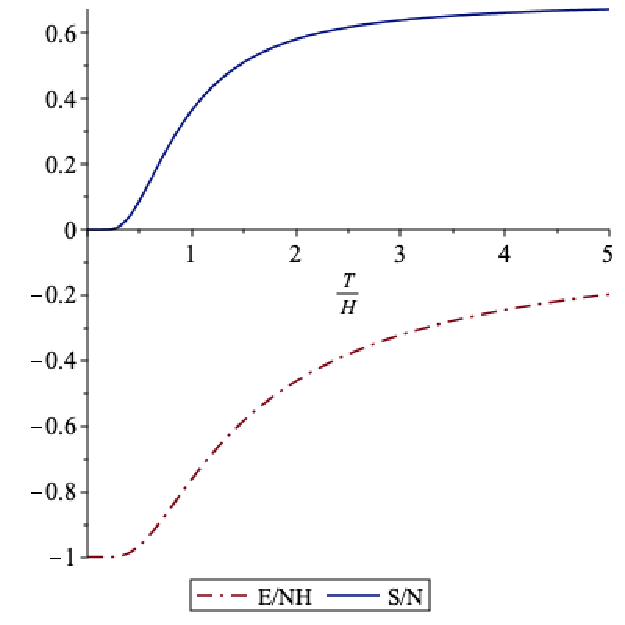
\includegraphics[width=0.7\textwidth]{figs/week03_distinguish.pdf}
\end{center}

Let's check the asymptotic behaviour of these functions, starting with \textbf{low temperatures}.
In the canonical ensemble, there is no issue with taking the independent variable $T \to 0$.
This corresponds to $\be H \to \infty$ and $\tanh\left(\be H\right) \to 1$, approaching the ``ground-state'' energy $E_{\text{min}} = E_0 = -NH$ you computed last week, which is realized only by the single micro-state in which all the spins are aligned with the magnetic field (every $s_n = -1$).
At the same time, $\log\left[2\cosh\left(\be H\right)\right] \to \log e^{\be H} = \be H$ and the two terms in \eq{eq:dist_entropy} cancel out, so that $S_D \to 0$.
This vanishing entropy is a generic consequence of temperatures approaching \textit{absolute zero}.

Even at low temperatures, $\vev{E}_D$ and $S_D$ will be affected by the non-zero probability for the system to adopt higher-energy ``excited states''.
Last week you also computed the energy $E_1 = -(N - 2)H$ of the first excited state, which is realized by $N$ distinct micro-states.
The \textit{energy gap} between the ground state and the first excited state is $\De E = E_1 - E_0 = 2H$.
(For this system all energy levels are separated by the same $E_{n_+ + 1} - E_{n_+} = 2H$, which we will use below.)

\newpage % WARNING: FORMATTING BY HAND
We can see the effects of the higher-energy states at low temperatures $\be H \gg 1$ by expanding $\vev{E}_D$ in powers of $e^{-\be H} \ll 1$.
What is the first $\frac{T}{H}$-dependent term in this expansion?
\begin{mdframed}
  $\displaystyle \frac{\vev{E}_D}{NH} = $ \\[100 pt]
\end{mdframed}
You should find that the excited-state effects are \textit{exponentially} suppressed by the energy gap $\De E$ at low temperatures,
\begin{equation*}
  \frac{\vev{E}_D}{NH} = -1 + 2e^{-\be \De E} + \cO\left(e^{-2\be \De E}\right).
\end{equation*}
This is a generic feature of systems with a non-zero energy gap, and is due to the exponentially small probability $\propto$$e^{-\be \De E}$ of the system adopting any of the micro-states with the higher energy.

The low-temperature expansion of \eq{eq:dist_entropy} for the entropy $S_D$ in powers of $e^{-\be H} \ll 1$ is similar:
\begin{mdframed}
  $\displaystyle \frac{S_D}{N} = $ \\[100 pt]
\end{mdframed}
Here the exponential suppression in the leading term is slightly counteracted by a linear factor of $\be \De E$,
\begin{equation*}
  \frac{S_D}{N} = \be \De E e^{-\be \De E} + e^{-\be \De E} + \cO\left(e^{-2\be \De E}\right).
\end{equation*}

In the limit of \textbf{high temperatures} the expansion of $\vev{E}_D$ and $S_D$ in powers of $\be H \ll 1$ is more straightforward.
The $\tanh$ in $\vev{E}_D$ can be expanded as usual,
\begin{equation*}
  \frac{\vev{E}_D}{NH} = -\tanh\left(\be H\right) = -\be H + \frac{\left(\be H\right)^3}{3} + \cO\left(\left[\be H\right]^5\right),
\end{equation*}
and vanishes $\sim$$\frac{1}{T}$ as $T \to \infty$.
This matches the micro-canonical behaviour we saw for this system last week, where the derived temperature diverged as the conserved energy approached zero.

For the entropy, there is a similar connection to micro-canonical behaviour at high temperatures:
\begin{mdframed}
  $\displaystyle \frac{S_D}{N} = $ \\[100 pt]
\end{mdframed}
As $\frac{T}{H} \to \infty$, the result
\begin{equation*}
  \frac{S_D}{N} = \log 2 - \frac{\left(\be H\right)^2}{2} + \cO\left(\left[\be H\right]^4\right)
\end{equation*}
approaches the asymptotic value $S_D \to N\log 2 = \log M$ for the $M = 2^N$ micro-states (with different energies).
Qualitatively, in this limit the energy of each spin is negligible compared to the temperature, and the system approximately behaves as though the energy were zero for all micro-states (and hence conserved).
% ------------------------------------------------------------------



% ------------------------------------------------------------------
\subsubsection{Indistinguishable spins in a gas}
We now consider nearly the same setup, with $N$ spins in thermodynamic equilibrium, in an external magnetic field of strength $H$.
The only difference is that now the spins are allowed to move, like particles in a one-dimensional gas.
We demand that they move slowly so that we can neglect their kinetic energy and the total energy of the system continues to be given by \eq{eq:spin_energy}.
Since the spins don't interact with each other, they can freely move past each other, and even occupy the same space, making it impossible for them to be distinguished from one another in any way. % Statistical treatment started by assuming we don't trace the motion of all the degrees of freedom...

To define the fundamental canonical partition function (\eq{eq:canon_part_func}), we have to sum over the micro-states of the system.
These micro-states are no longer in one-to-one correspondence with the full configurations $\left\{s_n\right\}$ of the $N$ spins.
Because the spins are now indistinguishable, certain spin configurations also cannot be distinguished from each other.
The simplest example comes from the two-spin system considered in \secref{sec:replicas}, where the configurations $\downarrow\uparrow$ and $\uparrow\downarrow$ now both map onto a single micro-state.
In this micro-state, we know only that one spin is $s_i = 1$ while the other is $s_k = -1$; it's not possible to distinguish which is which.

What remains observable is the energy of the micro-state.
Because permutations of the spin configurations don't change the internal energy (the sum in \eq{eq:spin_energy} is commutative), we can conclude that all such permutations correspond to a single distinct micro-state.
For this particular system, we saw above that the energies are best described as \textit{energy levels} separated by a constant gap $\De E = 2H$.
As a quick example, enumerate the energy levels when $N = 4$ and list the spin configurations associated with the corresponding micro-states.
How many micro-states are there for $N$ spins?
\begin{mdframed}
  \ \\[120 pt]
\end{mdframed}

A convenient way to label these micro-states and energy levels is to define
\begin{equation*}
  E_k = -NH + 2Hk
\end{equation*}
for micro-state $\om_k$ with $k = 0, \cdots N$.
(Previously we used the label $n_+$ instead of $k$.)
To compute the partition function $Z_I$ (with the subscript reminding us about the spins' indistinguishability), we simply sum
\begin{align}
  Z_I & = \sum_{k = 0}^N e^{-\be E_k} = \sum_{k = 0}^N e^{\be H (N - 2k)} = e^{N\be H} \sum_{k = 0}^N \left(e^{-2\be H}\right)^k = e^{N\be H} \frac{1 - e^{-2(N + 1) \be H}}{1 - e^{-2\be H}}.
\end{align}
The geometric series in the last step can be reconstructed by considering
\begin{equation*}
  \sum_{k = 0}^N x^k = \sum_{k = 0}^{\infty} x^k - \sum_{k = N + 1}^{\infty} x^k = \frac{1}{1 - x} - x^{N + 1} \sum_{\ell = 0}^{\infty} x^{\ell} = \frac{1}{1 - x} - \frac{x^{N + 1}}{1 - x}.
\end{equation*}

The corresponding Helmholtz free energy is
\begin{equation}
  \label{eq:indist_Helm}
  F_I(\be) = -NH - \frac{\log\left[1 - e^{-2(N + 1) \be H}\right]}{\be} + \frac{\log\left[1 - e^{-2 \be H}\right]}{\be}.
\end{equation}
In contrast to \eq{eq:dist_Helm}, $F_i(\be)$ is no longer proportional to $N$.
In a homework assignment you will use $F_I$ to determine the average internal energy $\vev{E}_I$ and entropy $S_I$ shown in the figures below, and also check the low- and high-temperature expansions like we did for the distinguishable case above.
Unlike our results for the distinguishable case, you will find that $\frac{\vev{E}_I}{NH}$ and $\frac{S_I}{N}$ depend on $N$, which requires us to fix $N = 4$ in the plots below.
\begin{center} % Don't need centering, but this will provide consistent vertical spacing
  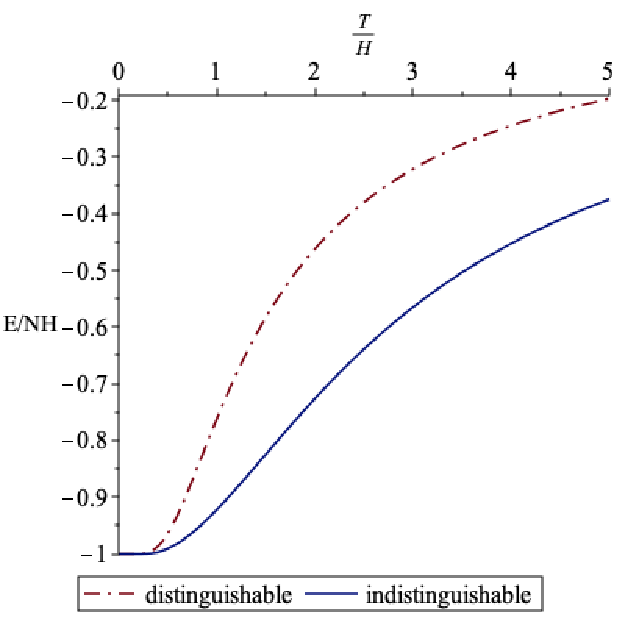
\includegraphics[width=0.45\textwidth]{figs/week03_energies.pdf}\hfill 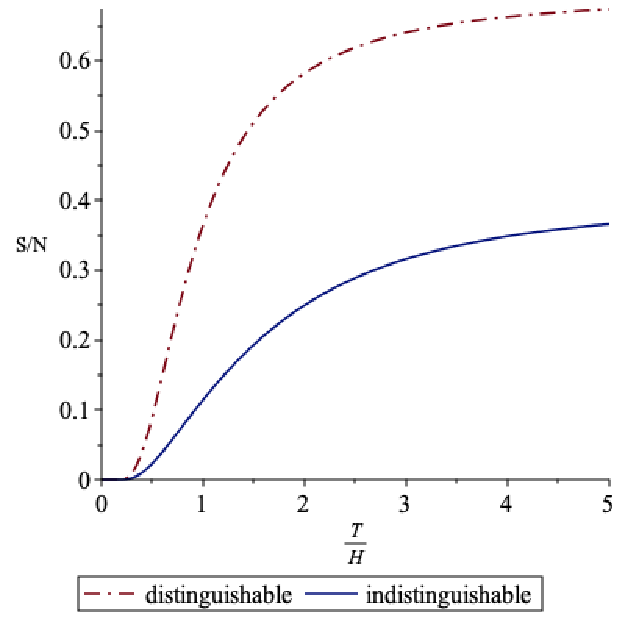
\includegraphics[width=0.45\textwidth]{figs/week03_entropies.pdf}
\end{center}

The dash-dotted lines in these figures are exactly the distinguishable-spin results shown above.
The solid lines are the new results for indistinguishable spins.
We see that the same $T \to 0$ limits are approached in both cases: $E \to -NH$ and $S \to 0$.
At low temperatures, the indistinguishable results approach these limits more quickly---they still feature exponential suppression of excited-state effects by the energy gap, $e^{-\be \De E}$, but this now comes with additional factors of $N$.

At high temperatures there is an even more striking difference.
While the average internal energy $\vev{E}_I$ continues to vanish $\sim$$\frac{1}{T}$ as $T \to \infty$ (with different $N$ dependence), the entropy approaches the asymptotic value $S_I \to \log\left(N + 1\right) = \log M$ for the $M = N + 1$ micro-states.
This logarithmic dependence on $N$ is very different from the $S_D \to N\log 2$ limit we found for distinguishable spins, and reflects the exponentially smaller number of micro-states that exist for indistinguishable spins, $N + 1$ vs.\ $2^N$.

Finally, away from those low- and high-temperature limits, the results above show a significant difference in the internal energy of the spin systems, depending only on whether or not the spins can be distinguished from each other in principle.
This is a physically measurable effect caused by the intrinsic information content of a statistical system, and a simple illustration of phenomena that remain at the leading edge of ongoing research.
The conclusion was pithily stated by \href{https://en.wikipedia.org/wiki/Rolf_Landauer}{Rolf Landauer} in 1991: ``Information is physical.''
% ------------------------------------------------------------------


\newpage
% ------------------------------------------------------------------
\renewcommand{\thisweek}{MATH327 Week 4}
\renewcommand{\moddate}{Last modified 15 Jan.~2021}
\setcounter{section}{4}
\section*{Week 4: Ideal gases}
\addcontentsline{toc}{section}{Week 4: Ideal gases}

\TODO{Being updated...}
% ------------------------------------------------------------------


\newpage
% ------------------------------------------------------------------
\renewcommand{\thisweek}{MATH327 Week 5}
\renewcommand{\moddate}{Last modified 25 Jan.~2021}
\setcounter{section}{5}
\phantomsection
\addcontentsline{toc}{section}{Week 5: Thermodynamic cycles}
\section*{Week 5: Thermodynamic cycles}

\TODO{Being written...}
% ------------------------------------------------------------------


\newpage
% ------------------------------------------------------------------
\renewcommand{\thisweek}{MATH327 Week 6}
\renewcommand{\moddate}{Last modified 8 Mar.~2021}
\setcounter{section}{6}
\setcounter{subsection}{0}
\phantomsection
\addcontentsline{toc}{section}{Week 6: Grand-canonical ensemble}
\section*{Week 6: Grand-canonical ensemble}
\subsection{The particle reservoir and chemical potential}
This week we define and develop the third and final statistical ensemble to be studied in this module, which is known as the grand-canonical ensemble.
Our approach will follow the pattern set by our previous development of the canonical ensemble.
Recall that statistical ensembles are probability spaces describing the micro-states that a system can adopt as it evolves in time, subject to certain constraints.
We began in week 2 with the micro-canonical ensemble, in which these constraints were conservation of the internal energy $E$ and particle number $N$.
We then introduced the canonical ensemble in week 3 by allowing the system's internal energy to fluctuate, while keeping its temperature $T$ fixed through thermal contact with a large external thermal reservoir.

The next step is to allow \textit{both} the system's energy and its particle number to fluctuate.
Just as we saw for the canonical ensemble in week 3, these fluctuations occur through contact between the system and a large external reservoir.
This is now a \textbf{particle reservoir}, with which the system can exchange both energy and particles.

In the same way that energy exchange leads to a fixed temperature, we expect there to be some quantity that will be fixed due to particle exchange.
Recall that we initially defined the temperature in the context of the micro-canonical ensemble in thermodynamic equilibrium (\eq{eq:temperature}), as the dependence of the entropy on the internal energy for a fixed number of degrees of freedom:
\begin{equation*}
  \frac{1}{T} = \left. \pderiv{S}{E}\right|_N.
\end{equation*}
The quantity we are now interested in comes from the complementary analysis interchanging the roles of $E$ and $N$.

\begin{shaded}
  In thermodynamic equilibrium, the \textbf{chemical potential} in the micro-canonical ensemble is defined by
  \begin{equation}
    \label{eq:chem_pot}
    \mu = -T \left. \pderiv{S}{N}\right|_E.
  \end{equation}
\end{shaded}

This definition is not terribly intuitive, nor is the chemical potential a familiar concept from everyday experiences.
To gain some insight into the chemical potential, we can note (from either \eq{eq:temperature} or \eq{eq:first_law}) that $\mu$ has dimensions of energy.
We can also expect the partial derivative $\pderiv{S}{N}$ to be positive in general, since systems with more degrees of freedom generically have more entropy, reflecting the greater amount of information they can contain.
This can be checked explicitly for the spin system (\eq{eq:dist_entropy}) and ideal gas (\eq{eq:ideal_entropy}) we previously analyzed.
The choice of sign in \eq{eq:chem_pot} therefore means that we should expect the chemical potential to be negative, in `natural' systems with positive temperatures.

The motivation for this negative sign comes from considering a net flow of particles between two systems $\Om_A$ and $\Om_B$ with the same temperature $T$ but different
\begin{equation*}
  \left(\pderiv{S}{N}\right)_A > \left(\pderiv{S}{N}\right)_B \qquad \Lra \qquad \mu_A < \mu_B.
\end{equation*}
Due to the negative sign in \eq{eq:chem_pot}, the system with the larger partial derivative has the smaller (more-negative) chemical potential.
According to the second law of thermodynamics, particles will flow from $\Om_B$ to $\Om_A$, because
\begin{equation*}
  \De S_A = \left(\pderiv{S}{N}\right)_A \De N > \left(\pderiv{S}{N}\right)_B \De N = \De S_B,
\end{equation*}
meaning that more entropy is gained by adding particles to system $\Om_A$ than is lost by removing particles from system $\Om_B$.
This ensures that the process increases the total entropy of the universe, $\De S = \De S_A - \De S_B > 0$.
In other words, we expect particles to flow \textit{from} systems with larger chemical potentials \textit{to} systems with smaller chemical potential.
This provides a useful similarity to heat flowing from hotter systems with larger temperatures to colder systems with smaller temperatures, allowing us to borrow our intuition from temperature to apply to the less-familiar chemical potential.\footnote{Of course, the mathematics would work just as well with the opposite sign convention---in that case we would just need to develop the opposite intuition for chemical potential vs.\ temperature.}
Like the temperature, the chemical potential is an intensive quantity.

\begin{shaded}
  We are now able to define a \textbf{grand-canonical ensemble} to be a statistical ensemble characterized by its fixed temperature $T$ and fixed chemical potential $\mu$, with the temperature and chemical potential held fixed through contact with a particle reservoir.
\end{shaded}
% ------------------------------------------------------------------



% ------------------------------------------------------------------
\subsection{\label{sec:Zg}The grand-canonical partition function}
We now place the grand-canonical ensemble on a more concrete mathematical foundation, following the same path as we did when developing the canonical ensemble.
That is, we introduce a well-motivated ansatz for the form of the particle reservoir $\Om_{\text{res}}$, then show that this specific form of $\Om_{\text{res}}$ is ultimately irrelevant.
This will allow us to work directly with the system of interest, $\Om$, independent of the details of the particle reservoir that fixes its temperature and chemical potential.

As before, our ansatz is to take $\Om_{\text{tot}} = \Om_{\text{res}} \otimes \Om$ to consist of many ($R \gg 1$) identical replicas of the system \Om that we're interested in.
All of these replicas are in thermodynamic equilibrium, and can exchange both energy and particles with each other.
The overall system $\Om_{\text{tot}}$ is governed by the micro-canonical ensemble, with conserved total energy \Etot and conserved total particle number $\Ntot$.
An extremely small example of this setup is illustrated by the figure below, where the system of interest is an ideal gas in a volume $V$.
This week we will consider only indistinguishable particles, so that we don't need to keep track of which particular particles are exchanged between the replicas, only the overall number.

\begin{center}
  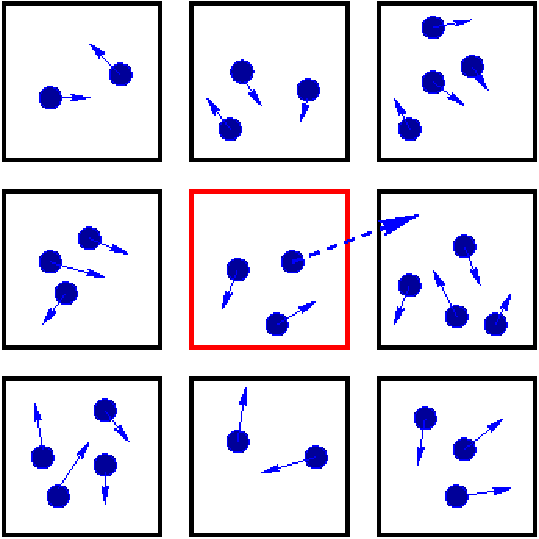
\includegraphics[width=0.7\textwidth]{figs/week06_reservoir.pdf}
\end{center}

Although we draw a box around each replica (and colour one red to pick out the system \Om we will consider), these boxes are now merely mental constructions, and don't interfere with particles moving from one replica to another.
For example, we could take our system to be a cubic centimetre of air in a room, with the rest of the room forming its reservoir.
As in \secref{sec:replicas}, we assume that this system $\Om = \left\{\om_1, \om_2, \cdots, \om_M\right\}$ has a finite number of $M$ possible micro-states, where now different micro-states may involve different numbers of particles.

This again allows us to analyze the overall system of $R$ replicas in terms of occupation numbers $n_i$ and the corresponding occupation probabilities $p_i$.
Recall that $n_i$ is the number of replicas that adopt the micro-state $\om_i \in \Om$ in any given micro-state of the overall system $\Om_{\text{tot}}$, so that $\sum_i n_i = R$.
Similarly, $p_i = n_i / R$ is the probability that a randomly chosen replica will be in micro-state $\om_i$, with $\sum_i p_i = 1$ as usual.
In terms of $n_i$ and $p_i$, the total number of micro-states of $\Om_{\text{tot}}$, and the corresponding entropy, are the same as we derived in \secref{sec:canon_part},
\begin{equation*}
  M_{\text{tot}} = \frac{R!}{n_1! \; n_2! \; \cdots \; n_M!} \qquad \lra \qquad S(\Etot, \Ntot) = -R \sum_{i = 1}^M p_i \log p_i,
\end{equation*}
assuming $R \gg 1$ and $n_i \gg 1$ for all $i = 1, \cdots, M$.
In this expression, the dependence on both \Etot and \Ntot now enters through the occupation probabilities $p_i$, since the micro-states $\om_i$ may involve different numbers of particles in addition to different energies.

Continuing as before, we want to determine the (intensive) temperature and chemical potential of $\Om_{\text{tot}}$ through Eqs.~\ref{eq:temperature} and \ref{eq:chem_pot}, which requires expressing $S(\Etot, \Ntot)$ directly in terms of \Etot and $\Ntot$.
We again do this by maximizing the entropy subject to the constraints on the conserved quantities of the micro-canonical overall system $\Om_{\text{tot}}$.
Labelling the energy and particle number of each replica $E_r$ and $N_r$, respectively, as in \eq{eq:canon_Etot} we can again rearrange sums over replicas into sums over the micro-states of $\Om$:
\begin{align}
  1 & = \sum_{i = 1}^M p_i & \Etot = \sum_{r = 1}^R E_r = \sum_{i = 1}^M n_i E_i & = R \sum_{i = 1}^M p_i E_i \cr
    &                      & \Ntot = \sum_{r = 1}^R N_r = \sum_{i = 1}^M n_i N_i & = R \sum_{i = 1}^M p_i N_i, \label{eq:grand_constraint}
\end{align}
where $E_i$ and $N_i$ are the energies and particle numbers of the $M$ micro-states $\om_i \in \Om$.
The first two constraints, on the occupation probabilities and the total energy, are the same as we had in \secref{sec:canon_part}.
The third constraint, on the total particle number, is the new ingredient for us to incorporate.

Writing everything in terms of occupation probabilities (choosing signs and normalization factors for later convenience), we see that we need to maximize the modified entropy
\begin{align*}
  \Sbar = -R \sum_{i = 1}^M p_i \log p_i & + \al\left(\sum_{i = 1}^M p_i - 1\right) \\
                                         & - \be\left(R \sum_{i = 1}^M p_i E_i - \Etot\right) + \ga\left(R \sum_{i = 1}^M p_i N_i - \Ntot\right),
\end{align*}
with the three Lagrange multipliers $\al$, \be and $\ga$.
What is the occupation probability $p_k$ that maximizes $\Sbar$?
\begin{mdframed}
  $\displaystyle 0 = \pderiv{\Sbar}{p_k} = $ \\[140 pt] % WARNING: FORMATTING BY HAND
\end{mdframed}

You should find a probability of the form
\begin{equation}
  \label{eq:grand_Lagrange}
  p_k = \frac{1}{Z_g} e^{-\be E_k + \ga N_k},
\end{equation}
defining $Z_g = \exp\left[1 - \frac{\al}{R}\right]$ to work in terms of the free parameters $\left\{Z_g, \be, \ga\right\}$.
As usual, we fix these three free parameters by demanding that the three constraints above are satisfied.
Using the first constraint, what is $Z_g$ in terms of \be and $\ga$?
\begin{mdframed}
  $\displaystyle 1 = \sum_{i = 1}^M p_i = $ \\[50 pt]
\end{mdframed}

Guided by our work in \secref{sec:canon_part}, we can expect to need the partial derivatives
\begin{align}
  \frac{1}{Z_g} \pderiv{}{\be} Z_g(\be, \ga) & = \frac{1}{Z_g} \pderiv{}{\be} \sum_{i = 1}^M e^{-\be E_i + \ga N_i} = -\frac{1}{Z_g} \sum_{i = 1}^M E_i \; e^{-\be E_i + \ga N_i} = -\frac{\Etot}{R} \label{eq:grand_be_deriv} \\
  \frac{1}{Z_g} \pderiv{}{\ga} Z_g(\be, \ga) & = \frac{1}{Z_g} \pderiv{}{\ga} \sum_{i = 1}^M e^{-\be E_i + \ga N_i} = \frac{1}{Z_g} \sum_{i = 1}^M N_i \; e^{-\be E_i + \ga N_i} = \frac{\Ntot}{R} \label{eq:grand_ga_deriv},
\end{align}
where we have used $\Etot = R \sum_i p_i E_i$ and $\Ntot = R \sum_i p_i N_i$ from \eq{eq:grand_constraint}.
These partial derivatives appear when we express the entropy in terms of $\Etot$, \Ntot and the free parameters
\begin{equation*}
  \left\{Z_g(\be, \ga), \quad \be(\Etot, \Ntot), \quad \ga(\Etot, \Ntot)\right\},
\end{equation*}
then take the partial derivatives that define the temperature and chemical potential.
What do you obtain upon inserting \eq{eq:grand_Lagrange} for $p_i$ into the formula for the entropy?
\begin{mdframed}
  $\displaystyle S(\Etot, \Ntot) = -R \sum_{i = 1}^M p_i \log p_i = $ \\[100 pt]
\end{mdframed}

\newpage % WARNING: FORMATTING BY HAND
Taking the derivative of the result with respect to $\Etot$, keeping \Ntot fixed, gives us the temperature (\eq{eq:temperature}):
\begin{align}
  \frac{1}{T} & = \pderiv{}{\Etot}\left[R\log Z_g + \be \Etot - \ga \Ntot\right]_{\Ntot} \cr
              & = \frac{R}{Z_g}\left(\pderiv{Z_g}{\be}\pderiv{\be}{\Etot} + \pderiv{Z_g}{\ga}\pderiv{\ga}{\Etot}\right) + \Etot\pderiv{\be}{\Etot} + \be - \Ntot\pderiv{\ga}{\Etot} \cr
              & = -\Etot\pderiv{\be}{\Etot} + \Ntot\pderiv{\ga}{\Etot} + \Etot\pderiv{\be}{\Etot} + \be - \Ntot\pderiv{\ga}{\Etot} = \be,
\end{align}
where we insert Eqs.~\ref{eq:grand_be_deriv} and \ref{eq:grand_ga_deriv} in the last line.
In the same way, the derivative with respect to $\Ntot$, keeping $\Etot$ fixed, gives us the chemical potential:
\begin{align}
  \mu & = -T \pderiv{}{\Ntot}\left[R\log Z_g + \be \Etot - \ga \Ntot\right]_{\Ntot} \cr
      & = -T\left[\frac{R}{Z_g}\left(\pderiv{Z_g}{\be}\pderiv{\be}{\Ntot} + \pderiv{Z_g}{\ga}\pderiv{\ga}{\Ntot}\right) + \Etot\pderiv{\be}{\Ntot} - \Ntot\pderiv{\ga}{\Ntot} - \ga\right] \cr
      & = -T\left[-\Etot\pderiv{\be}{\Ntot} + \Ntot\pderiv{\ga}{\Ntot} + \Etot\pderiv{\be}{\Ntot} - \Ntot\pderiv{\ga}{\Ntot} - \ga\right] = T\ga.
\end{align}

Putting everything together, we have
\begin{align}
  \be & = \frac{1}{T} &
  \ga & = \be \mu = \frac{\mu}{T}
\end{align}
and the desired result that all the details of the particle reservoir have vanished, with no remaining reference to $R$, \Etot or $\Ntot$.
The large particle reservoir is still present to fix the temperature $T$ and chemical potential $\mu$ that characterize the grand-canonical system $\Om$, but beyond that nothing about it is relevant---or even knowable in the grand-canonical approach.

Every aspect of \Om can now be specified in terms of its fixed temperature $T$ and chemical potential $\mu$, starting with the parameters $\be = 1 / T$ and $\ga = \mu / T$.
In particular, the probability---in thermodynamic equilibrium---that \Om adopts micro-state $\om_i$ with (non-conserved) internal energy $E_i$ and particle number $N_i$ is
\begin{equation}
  \label{eq:grand_prob}
  p_i = \frac{1}{Z_g} e^{-\be (E_i - \mu N_i)} = \frac{1}{Z_g} e^{-(E_i - \mu N_i) / T}.
\end{equation}

\begin{shaded}
  These probabilities depend on the \textbf{grand-canonical partition function}
  \begin{equation}
    \label{eq:grand_part_func}
    Z_g(T, \mu) = \sum_{i = 1}^M e^{-\be (E_i - \mu N_i)} = \sum_{i = 1}^M e^{-(E_i - \mu N_i) / T}.
  \end{equation}
  Analogously to the canonical partition function, this $Z_g$ is a fundamental quantity in the grand-canonical ensemble, from which many other derived quantities can be obtained.
\end{shaded}

Since the particle number $N_i$ is dimensionless, the combination $E_i - \mu N_i$ that appears in Eqs.~\ref{eq:grand_prob} and \ref{eq:grand_part_func} is consistent with our observation below \eq{eq:chem_pot} that the chemical potential $\mu$ has dimensions of energy.
% ------------------------------------------------------------------



% ------------------------------------------------------------------
\subsection{The grand-canonical potential, internal energy, entropy, and particle number}
The development of the grand-canonical ensemble we have seen so far closely resembles our earlier work setting up the canonical ensemble.
We have generalized the thermal reservoir to a particle reservoir that allows both the internal energy and particle number of the system \Om to vary, while keeping its temperature $T$ and chemical potential $\mu$ fixed.
By adapting the replica ansatz to this setup, we determined the grand-canonical partition function $Z_g$, and found it to be independent of the details of the particle reservoir.

We now continue by considering a similar set of derived quantities for the grand-canonical ensemble in thermodynamic equilibrium.
In addition to the expectation value of the internal energy introduced in \secref{sec:canon_derived}, the fluctuations of the particle number mean that we also need to consider its expectation value,
\begin{align*}
  \vev{E}\!(T, \mu) & = \sum_{i = 1}^M E_i \; p_i = \frac{1}{Z_g} \sum_{i = 1}^M E_i \; e^{-\be (E_i - \mu N_i)} \\
  \vev{N}\!(T, \mu) & = \sum_{i = 1}^M N_i \; p_i = \frac{1}{Z_g} \sum_{i = 1}^M N_i \; e^{-\be (E_i - \mu N_i)}.
\end{align*}
We can anticipate that both of these derived quantities will be related to the logarithm of the grand-canonical partition function, in analogy to the Helmholtz free energy for the canonical ensemble considered in \secref{sec:Helmholtz}.

\begin{shaded}
  This leads us to define \textbf{grand-canonical potential} of a grand-canonical ensemble to be
  \begin{equation}
    \label{eq:grand_pot}
    \Phi(T, \mu) = -T \log Z_g(T, \mu) = -\frac{\log Z_g(\be, \mu)}{\be},
  \end{equation}
  where $Z_g$ is the grand-canonical partition function of the ensemble.
  In terms of this free energy, Eqs.~\ref{eq:grand_prob} and \ref{eq:grand_part_func} are
  \begin{align*}
    Z_g & = e^{-\Phi / T} &
    p_i & = e^{(\Phi - E_i + \mu N_i) / T}.
  \end{align*}
\end{shaded}

The grand-canonical potential is sometimes called the \textit{Landau free energy}, named after \href{https://en.wikipedia.org/wiki/Lev_Landau}{Lev Landau}, to highlight its similarity with the Helmholtz free energy.
\newpage % WARNING: FORMATTING BY HAND
\noindent An aspect of this similarity is the importance of derivatives of the grand-canonical potential.
The simplest derivative to consider first is with respect to the chemical potential,
\begin{mdframed}
  $\displaystyle \pderiv{}{\mu} \Phi(\be, \mu) = $ \\[120 pt]
\end{mdframed}
The derivative with respect to the temperature is a little messier.
As in \secref{sec:Helmholtz}, it involves $\pderiv{}{T} \log Z_g$, which is again worth collecting in advance, recalling $\pderiv{}{T} = -\be^2 \pderiv{}{\be} $ from \eq{eq:beta_T}.
\begin{mdframed}
  $\displaystyle -\pderiv{}{T}\left(\frac{\Phi(T, \mu)}{T}\right) = \pderiv{}{T} \log Z_g(T, \mu) = $ \\[80 pt]
  $\displaystyle \pderiv{}{T} \Phi(T, \mu) = $ \\[80 pt]
\end{mdframed}
\newpage % WARNING: FORMATTING BY HAND
\noindent You should find
\begin{equation*}
  \pderiv{\Phi}{T} = \frac{\Phi - \vev{E} + \mu\vev{N}}{T} = -\log Z_g - \be\vev{E} + \be\mu\vev{N},
\end{equation*}
which we can connect to the entropy by inserting the probabilities $p_i$ from \eq{eq:grand_prob} into the definition of the entropy from \eq{eq:entropy}:
\begin{mdframed}
  $\displaystyle S(T, \mu) = -\sum_{i = 1}^M p_i \log p_i = $ \\[100 pt]
\end{mdframed}

\begin{shaded}
  From this work we can read off the following relations involving the grand-canonical potential $\Phi(T, \mu)$:
  \begin{align}
    \vev{N}\!(T, \mu) & = -\pderiv{}{\mu} \Phi(T, \mu) \label{eq:N_grand} \\
            S(T, \mu) & = -\pderiv{}{T} \Phi(T, \mu) \\
    \vev{E}\!(T, \mu) & = -T^2 \pderiv{}{T} \left[\frac{\Phi(T, \mu)}{T}\right] + \mu \vev{N}\!(T, \mu) \label{eq:E_grand} \\
         \Phi(T, \mu) & = -T S(T, \mu) + \vev{E}\!(T, \mu) - \mu \vev{N}\!(T, \mu) \label{eq:grand_relation}
  \end{align}
\end{shaded}

Finally, the connections between the energy, entropy and particle number provided by these relations motivate a further extension of the general first law of thermodynamics we derived last week (\eq{eq:first_law}).
Now allowing the particle number $N$ of our thermodynamic system to change, we can express its entropy as a function of the internal energy, volume and particle number, $S(E, V, N)$, and consider the change in the entropy due to changes in each of these three parameters,\footnote{To make the notation less cumbersome here, we write $\vev{E}$ and $\vev{N}$ as $E$ and $N$, respectively, keeping in mind that these are properties of the system's thermodynamic macro-state rather than its fluctuating micro-state.}
\begin{equation*}
  dS = \left.\pderiv{S}{E}\right|_{V, N} dE + \left.\pderiv{S}{V}\right|_{E, N} dV + \left.\pderiv{S}{N}\right|_{V, E} dN = \frac{1}{T} dE + \left.\pderiv{S}{V}\right|_{E, N} dV - \frac{\mu}{T} dN.
\end{equation*}
We can interpret the remaining partial derivative by considering the first law, \eq{eq:first_law}, in the case of fixed internal energy $E$,
\begin{equation*}
  dE = 0 = T \; dS - P \; dV \qquad \Lra \qquad \left.\pderiv{S}{V}\right|_{E, N} = \frac{P}{T}.
\end{equation*}
The fixed particle number $N$ is already incorporated into \eq{eq:first_law}, since that expression was derived in the framework of the canonical ensemble.

Putting things together, we obtain the generalized thermodynamic identity
\begin{equation}
  \label{eq:thermo_ident}
  dE = T \; dS - P \; dV + \mu \; dN.
\end{equation}
Due to this result, the term $\mu \; dN$ is sometimes referred to as ``chemical work'', in analogy to the mechanical work $W = - P \; dV$ done on the system by changing its volume.
This thermodynamic identity provides a convenient way to remember (or derive) relations between the internal energy, entropy, volume and particle number in thermodynamic equilibrium, by considering processes in which any two of these are fixed.
For example, fixing $N$ and $V$ gets us back to \eq{eq:temperature} for the temperature,
\begin{equation*}
  dE = T \; dS \qquad \Lra \qquad \frac{1}{T} = \left.\pderiv{S}{E}\right|_{N, V},
\end{equation*}
while fixing $N$ and $S$ gives \eq{eq:pressure} for the pressure,
\begin{equation*}
  dE = -P \; dV \qquad \Lra \qquad P = -\left.\pderiv{E}{V}\right|_{N, S}.
\end{equation*}

If we fix the entropy $S$ and volume $V$, we end up with another way of understanding the chemical potential,
\begin{equation}
  \label{eq:mu_E}
  dE = \mu \; dN \qquad \Lra \qquad \mu = \left.\pderiv{E}{N}\right|_{S, V}.
\end{equation}
That is, the chemical potential is the change in the internal energy when we adiabatically add a particle to the system (in a constant volume).
We argued below \eq{eq:chem_pot} that systems with more degrees of freedom generically have more entropy, and can recall that `natural' systems have positive temperatures that correspond to the entropy increasing as the internal energy increases.
In order to keep the entropy \textit{fixed} as we increase $N$, we would therefore have to reduce $E$, and vice-versa, so that \eq{eq:mu_E} confirms our earlier finding that the chemical potential is negative in general.
% ------------------------------------------------------------------


\newpage
% ------------------------------------------------------------------
\renewcommand{\thisweek}{MATH327 Week 7}
\renewcommand{\moddate}{Last modified 11 Apr.~2021}
\setcounter{section}{7}
\setcounter{subsection}{0}
\phantomsection
\addcontentsline{toc}{section}{Week 7: Quantum statistics}
\section*{Week 7: Quantum statistics}
\subsection{\label{sec:quantum}Quantized energy levels and their micro-states}
This week we begin applying the grand-canonical ensemble to investigate quantum statistical systems.
The first step is to introduce quantum statistics itself, building on the initial glimpse that we got in \secref{sec:regulate}.
It is worth reiterating that no prior knowledge of quantum physics is assumed, nor will this module attempt to teach quantum mechanics.
We will simply consider quantum behaviour as an ansatz (that turns out to be realized in nature), and analyze the resulting systems by making use of the statistical physics tools we have developed.

Looking back to our derivation of the canonical partition function for a classical (that is, non-quantum) ideal gas in \secref{sec:regulate}, we can recall that we engaged in slightly circular argumentation.
First, because the partition function is defined as a sum over micro-states $\om_i$,
\begin{equation*}
  Z = \sum_i e^{-E(\vec{p}_i) / T},
\end{equation*}
we had to conjecture that the gas particles' momenta $\vec{p}_i$ are \textit{quantized} and can take only particular discrete values, rather than varying continuously.
These quantized momenta produce a countable number of discrete \textit{energy levels}, leading to a countable number of micro-states and hence a well-defined partition function that takes the form of a sum over all possible discrete momenta for each particle.
Second, we then assumed that the energy levels are spaced very close to each other, allowing us to approximate that sum as a multi-dimensional gaussian integral.
That is, we went right back to working with continuously varying momenta, despite the formal need to regulate the system by quantization.

For the next few weeks, we will work in the quantum regime where all energy levels of a system remain discrete.
In addition, a more subtle change of approach is required by the fundamental indistinguishability of particles governed by quantum mechanics.
This quantum indistinguishability is a fact about nature that we will take as given.

To appreciate the consequences of quantum indistinguishability, let's first apply our usual (classical) approach to compute the grand-canonical partition function for a system with discrete energy levels.
Despite the quantized energy levels, this calculation will still produce a non-quantum result known as \textbf{Maxwell--Boltzmann} (MB) statistics (named after \href{https://en.wikipedia.org/wiki/James_Clerk_Maxwell}{James Clerk Maxwell} and Ludwig Boltzmann).
We will be able to see when this result is a good approximation and when it breaks down.

To define some notation, let's label the discrete energy levels $\cE_{\ell}$ for $\ell = 0$, $1$, $\cdots$, $L$, where $L$ can be taken to infinity while retaining a countable number of micro-states and hence well-defined partition functions.
The energy level $\cE_{\ell}$ may be characterized by extra information in addition to the actual value of its energy, $E_{\ell}$.
As we saw in \secref{sec:regulate}, it is therefore possible for distinct energy levels $\left\{\cE_m, \cE_n\right\}$ to have the same energy $E_m = E_n$ for $m \neq n$.
Such energy levels with the same value of the energy are said to be \textit{degenerate}.
We will label energy levels so that $E_m \leq E_n$ for $m < n$.
Without loss of generality, we can take $E_{\ell} \geq E_0 \geq 0$.

Now starting from the general expression for the grand-canonical partition function, \eq{eq:grand_part_func},
\begin{equation*}
  Z_g(\be, \mu) = \sum_i e^{-\be (E_i - \mu N_i)},
\end{equation*}
we just need to define the micro-states $\om_i$ with energy $E_i$ and particle number $N_i$.
In the classical Maxwell--Boltzmann approach, we first sum over all possible particle numbers,
\begin{equation*}
  \ZMB(\be, \mu) = \sum_{i, N_i = 0} e^{-\be E_i} + \sum_{j, N_j = 1} e^{-\be (E_j - \mu)} + \sum_{k, N_k = 2} e^{-\be (E_k - 2\mu)} + \cdots,
\end{equation*}
where the micro-states labelled $\left\{\om_i, \om_j, \om_k, \cdots\right\}$ are those that have $N = 0$, $1$, $2$, $\cdots$ particles, respectively.
We can recognize $N$-particle canonical partition functions $Z_N(\be)$ in the expression above,
\begin{equation}
  \label{eq:fugacity_exp}
  \ZMB(\be, \mu) = Z_0(\be) + e^{\be\mu} Z_1(\be) + e^{2\be\mu} Z_2(\be) + \cdots = \sum_{N = 0}^{\infty} \left[e^{\be\mu}\right]^N Z_N(\be),
\end{equation}
allowing us to benefit from our experience with the canonical ensemble.
(This is a general result known as the \textit{fugacity expansion}, where $e^{\be\mu}$ is called the fugacity.)

In particular, because we continue to consider only `ideal' systems in which the particles don't interact with each other, each $Z_N(\be)$ is simply the product of the single-particle partition functions $Z_1(\be)$ for all $N$ independent particles,
\begin{equation*}
  Z_N(\be) = \frac{1}{N!} \left[Z_1(\be)\right]^N,
\end{equation*}
with the factor of $N!$ included to correct for over-counting indistinguishable particles.
This is exactly the derivation we performed in \secref{sec:regulate}, to obtain \eq{eq:ideal_indis} for the classical ideal gas.
Inserting this into \eq{eq:fugacity_exp}, we have
\begin{equation*}
  \ZMB(\be, \mu) = \sum_{N = 0}^{\infty} \frac{1}{N!} \left[e^{\be\mu}\right]^N \left[Z_1(\be)\right]^N = \sum_{N = 0}^{\infty} \frac{1}{N!} \left[e^{\be\mu} Z_1(\be)\right]^N = \exp\left[e^{\be\mu} Z_1(\be)\right].
\end{equation*}
In the case of a system with discrete energy levels $E_{\ell}$, the single-particle partition function is simply
\begin{equation*}
  Z_1(\be) = \sum_{\ell = 0}^L e^{-\be E_{\ell}},
\end{equation*}
leading to the Maxwell--Boltzmann grand-canonical partition function
\begin{equation}
  \label{eq:partfunc_MB_nonfactor}
  \ZMB(\be, \mu) = \exp\left[e^{\be\mu} \sum_{\ell = 0}^L e^{-\be E_{\ell}} \right] = \exp\left[\sum_{\ell = 0}^L e^{-\be\left(E_{\ell} - \mu\right)}\right].
\end{equation}

Unfortunately, as mentioned in a footnote accompanying \eq{eq:ideal_indis}, this derivation relies on the assumption that every particle occupies a different energy level.
While this would be effectively guaranteed when the particles' energies vary continuously, and can be an excellent approximation when there are many more energy levels than there are particles to occupy them, the assumption breaks down if there is a non-negligible chance of two particles occupying the same energy level.

We can illustrate this with a simple exercise of considering a system with $N = 2$ particles that can occupy any of five energy levels.
For a further simplification, let's suppose that all five energy levels are degenerate, with $E_{\ell} = 0$ for $\ell = 0$, $\cdots$, $5$.
This means the canonical partition function simply counts the (integer) number of micro-states, for example
\begin{equation*}
  Z_1 = \sum_{\ell = 0}^4 e^{-\be E_{\ell}} = \sum_{\ell = 0}^4 1 = 5
\end{equation*}
for all $\be = 1 / T$.
The mathematics is the same as counting the number of ways two balls can be placed in five boxes, with possible micro-states that can be represented as $\boxzero\boxone\boxzero\boxzero\boxone$ and $\boxzero\boxzero\boxtwo\boxzero\boxzero$.
What is the two-particle partition function if the balls are distinguishable?
\begin{mdframed}
  $Z_D = $ \\[24 pt]
\end{mdframed}
For indistinguishable particles, our derivation above would predict the partition function $Z_I = \frac{1}{2} Z_D$, which is not an integer and therefore cannot be correct.

We can spot the error by explicitly writing down all micro-states in both cases of distinguishable and indistinguishable particles.
In the distinguishable case, we can suppose that the balls are red ($\textcolor{red}{\bullet}$) and blue ($\textcolor{blue}{\bullet}$), and compactly label micro-states by recording whether each box is empty (``$0$''), contains the red ball (``$R$''), the blue ball (``$B$'') or both balls (``$2$''):
\begin{align*}
  \boxzero\boxzero\boxed{\textcolor{red}{\bullet}}\boxzero\boxed{\textcolor{blue}{\bullet}} & = 00R0B &
  \boxzero\boxzero\boxed{\textcolor{red}{\bullet}\textcolor{blue}{\bullet}}\boxzero\boxzero & = 00200.
\end{align*}
The full catalog of micro-states is then
\begin{align*}
  RB000 & & 0R0B0 & & BR000 & & 0B0R0 & & 20000 \\
  R0B00 & & 0R00B & & B0R00 & & 0B00R & & 02000 \\
  R00B0 & & 00RB0 & & B00R0 & & 00BR0 & & 00200 \\
  R000B & & 00R0B & & B000R & & 00B0R & & 00020 \\
  0RB00 & & 000RB & & 0BR00 & & 000BR & & 00002
\end{align*}
If we now consider indistinguishable particles where we can only know the number $R = B = 1$, we see that the third and fourth columns above duplicate the first two columns.
This is exactly the over-counting that the usual factor of $\frac{1}{N!} = \frac{1}{2}$ corrects, which leaves us with the micro-states
\begin{align*}
  11000 & & 01010 & & 20000 \\
  10100 & & 01001 & & 02000 \\
  10010 & & 00110 & & 00200 \\
  10001 & & 00101 & & 00020 \\
  01100 & & 00011 & & 00002
\end{align*}
But we see that the micro-states in the final column, with both particles in the same energy level, were not over-counted, and must not be divided by $N!$.

In order to generalize this simple exercise, we note that the micro-states for indistinguishable particles can be systematically labelled by \textit{occupation numbers} $n_{\ell}$, similar to those that we encountered when using replicas to derive the canonical partition function in \secref{sec:reservoir} and the grand-canonical partition function in \secref{sec:Zg}.
Here the occupation number $n_{\ell}$ is simply the number of particles in energy level $\cE_{\ell}$.
This change of perspective is all we need to define quantum statistics as opposed to classical statistics.

\begin{shaded}
  In \textbf{quantum statistics}, the micro-states are defined by considering each energy level $\cE_{\ell}$ in turn, and summing over the possible occupation numbers $n_{\ell}$ that it could have.
  This contrasts with the classical approach in which we define the micro-states by considering each particle in turn, and summing over the possible energies $E_{\ell}$ that it could have.
\end{shaded}

Recalling the fundamental indistinguishability of particles governed by quantum mechanics, we have seen that the classical approach over-counts micro-states, but this over-counting depends on how likely it is for multiple particles to occupy the same energy level.
The quantum approach of summing over the occupation numbers of the quantized energy levels avoids this issue, and requires no additional factors to correct over-counting.
% ------------------------------------------------------------------



% ------------------------------------------------------------------
\subsection{Bosons and fermions}
In the two sections below we will carry out explicit computations to clarify what the above definition of quantum statistics means in practice.
First, there is one more fact about nature that we need to mention.
This concerns the occupation numbers $n_{\ell}$ that are possible for each energy level $\cE_{\ell}$.

\href{https://en.wikipedia.org/wiki/Spin-statistics_theorem}{A theorem}, based on quantum mechanics and special relativity, states that all particles are either \textit{bosons} (named after \href{https://en.wikipedia.org/wiki/Satyendra_Nath_Bose}{Satyendra Nath Bose}) or \textit{fermions} (named after \href{https://en.wikipedia.org/wiki/Enrico_Fermi}{Enrico Fermi}).\footnote{The proof assumes three-dimensional physical space, and \href{https://en.wikipedia.org/wiki/Anyon}{more exotic behaviour} is possible for particles confined to two-dimensional surfaces.}
These two classes of particles obey different rules for their possible occupation numbers, and therefore give rise to distinct quantum statistics.

Any non-negative number of identical bosons can simultaneously occupy the same energy level, corresponding to occupation numbers $n_{\ell} = 0$, $1$, $2$, $\cdots$.
Physical examples of bosons include photons (particles of light), pions, helium-$4$ atoms and the famous Higgs particle.

On the other hand, it is impossible for multiple identical fermions to occupy the same energy level, meaning that their only possible occupation numbers are $n_{\ell} = 0$ and $1$.
This behaviour is known as the \textit{Pauli exclusion principle} (named after \href{https://en.wikipedia.org/wiki/Wolfgang_Pauli}{Wolfgang Pauli}) and has extremely important consequences, including the existence of chemistry and life.
Physical examples of fermions include electrons, protons, neutrons, neutrinos and helium-$3$ atoms.

The reason multiple identical fermions cannot occupy the same energy level is due to a feature of quantum mechanics, and not because they physically repel each other.
This paragraph will imprecisely describe that aspect of quantum physics for the curious, and can be skipped without any problem.
Consider a system of identical quantum particles occupying various energy levels.
Loosely speaking, if we interchange any pair of those particles, we end up with the same system, up to a factor of $\pm 1$.
Bosons correspond to the intuitive $+1$ case, where interchanging indistinguishable particles has no effect.
Fermions correspond to the unintuitive $-1$ case (which is related to \href{https://en.wikipedia.org/wiki/Grassmann_number}{Grassmann numbers} named after \href{https://en.wikipedia.org/wiki/Hermann_Grassmann}{Hermann Grassmann}).
In this case, if the particles we interchange are occupying the same energy level, the resulting system is exactly the same as the starting point --- but it also has to differ by this factor of $-1$.
Since no non-zero system of particles can equal its negative, no systems with multiple identical fermions in the same energy level can possibly exist.

Looking back at the example system of $N = 2$ particles with five energy levels in the previous section, all $15$ micro-states we wrote down are possible if the particles are bosons.
Which of those micro-states are allowed if the particles are fermions?
\begin{mdframed}
  \ \\[24 pt]
\end{mdframed}
This difference in the possible micro-states ensures that bosons and fermions exhibit different quantum statistics.
We will now consider each case in turn.
% ------------------------------------------------------------------



% ------------------------------------------------------------------
\subsection{Bose--Einstein statistics}
The quantum statistics of bosons is known as \textbf{Bose--Einstein} (BE) statistics, named after Satyendra Nath Bose and Albert Einstein.
As described above, to carry out the sum over all micro-states in the grand-canonical partition function
\begin{equation*}
  Z_g(\be, \mu) = \sum_i e^{-\be (E_i - \mu N_i)},
\end{equation*}
we first sum over all energy levels $\cE_{\ell}$, and then over all possible occupation numbers $n_{\ell} \in \Nbb_0$ for each energy level.

Consider first the simple case of a system that only has a single energy level $\cE$, with energy $E$.
In this case, each micro-state $\om_i$ is uniquely described by its particle number $N_i$, which is just the occupation number of $\cE$.
What is the energy $E_i$ of micro-state $\om_i$ with occupation number $n = N_i$?
\begin{mdframed}
  $E_i = $ \\[24 pt]
\end{mdframed}

Plugging this into the sum over all possible particle numbers, the Bose--Einstein grand-canonical partition function for this single-level system is
\begin{equation}
  \label{eq:BEsingle}
  \ZBE(\be, \mu) = \sum_{n = 0}^{\infty} e^{-\be (E - \mu) n} = \sum_{n = 0}^{\infty} \left[e^{-\be (E - \mu)}\right]^n = \frac{1}{1 - e^{-\be (E - \mu)}}.
\end{equation}
In the last step we recognized the geometric series
\begin{equation*}
  \frac{1}{1 - x} = 1 + x + x^2 + \cdots,
\end{equation*}
which only converges for $x = e^{-\be (E - \mu)} < 1$.
For natural systems with $\be = 1 / T > 0$, this condition requires $E - \mu > 0$ or equivalently $\mu < E$.
Since we can also take $E_{\ell} \geq 0$ without loss of generality, this constraint is consistent with the negative chemical potential $\mu < 0$ that we discussed last week.

At this point, it is straightforward to generalize to multiple energy levels $\cE_{\ell}$ with $\ell = 0$, $1$, $\cdots$, $L$.
Because we consider only ideal systems with non-interacting particles, the micro-state $\om_i$ defined by the set of occupation numbers $\left\{n_{\ell}\right\}$ has total energy and particle number
\begin{align}
  \label{eq:total_energy_levels}
  E_i & = \sum_{\ell = 0}^L E_{\ell} n_{\ell} &
  N_i & = \sum_{\ell = 0}^L n_{\ell}.
\end{align}
The general Bose--Einstein grand-canonical partition function is therefore
\begin{equation*}
  \ZBE(\be, \mu) = \sum_{n_0 = 0}^{\infty} \sum_{n_1 = 0}^{\infty} \cdots \sum_{n_L = 0}^{\infty} \exp\left[-\be\sum_{\ell = 0}^L \left(E_{\ell} - \mu\right) n_{\ell}\right].
\end{equation*}
We can apply the identity $e^{\sum_i x_i} = \prod_i e^{x_i}$ to rewrite
\begin{equation*}
  \exp\left[-\be\sum_{\ell = 0}^L \left(E_{\ell} - \mu\right) n_{\ell}\right] = \left(e^{-\be (E_0 - \mu) n_0}\right) \left(e^{-\be (E_1 - \mu) n_1}\right)\cdots \left(e^{-\be (E_L - \mu) n_L}\right).
\end{equation*}
Recalling $\mu < E_{\ell}$ for all $\ell$, by rearranging the terms we find
\begin{align}
  \ZBE(\be, \mu) & = \left(\sum_{n_0 = 0}^{\infty} e^{-\be (E_0 - \mu) n_0}\right) \left(\sum_{n_1 = 0}^{\infty} e^{-\be (E_1 - \mu) n_1}\right)\cdots \left(\sum_{n_L = 0}^{\infty} e^{-\be (E_L - \mu) n_L}\right) \cr
                 & = \prod_{\ell = 0}^L \frac{1}{1 - e^{-\be (E_{\ell} - \mu)}}. \label{eq:partfunc_BE}
\end{align}

This grand-canonical partition function defines the quantum Bose--Einstein statistics of bosons.
Its structure as the product of an independent contribution for each energy level is reminiscent of the result $Z_N \propto Z_1^N$ for the classical $N$-particle canonical partition function discussed in \secref{sec:quantum}.
In both cases we say that the computation \textit{factorizes} into a product of many similar pieces, which can enable drastic simplifications.
Looking back to \eq{eq:partfunc_BE}, we can also observe factorization in the classical Maxwell--Boltzmann grand-canonical partition function,
\begin{equation}
  \label{eq:partfunc_MB}
  \ZMB(\be, \mu) = \exp\left[\sum_{\ell = 0}^L e^{-\be\left(E_{\ell} - \mu\right)}\right] = \prod_{\ell = 0}^L \exp\left[e^{-\be\left(E_{\ell} - \mu\right)}\right].
\end{equation}
In all of these cases, factorization is possible because the particles are non-interacting.
In a few weeks we will consider non-ideal systems in which the particles can interact with each other, where the absence of factorization will make analyses much more difficult.
% ------------------------------------------------------------------



% ------------------------------------------------------------------
\subsection{\label{sec:fermi}Fermi--Dirac statistics}
The quantum statistics of fermions is known as \textbf{Fermi--Dirac} (FD) statistics, named after Enrico Fermi and \href{https://en.wikipedia.org/wiki/Paul_Dirac}{Paul Dirac}.
The derivation of the Fermi--Dirac grand-canonical partition function is very similar to the Bose--Einstein case considered in the previous section.
We again proceed by summing over all energy levels $\cE_{\ell}$, and just have to account for the more limited possible occupation numbers $n_{\ell} \in \left\{0, 1\right\}$ for each energy level.

Taking the same approach of first considering a simple system with only a single energy level, \eq{eq:BEsingle} would just change to
\begin{equation*}
  \ZFD(\be, \mu) = \sum_{n = 0}^1 e^{-\be (E - \mu) n} = 1 + e^{-\be (E - \mu)}.
\end{equation*}
Generalizing to multiple energy levels $\cE_{\ell}$ with $\ell = 0$, $1$, $\cdots$, $L$, the energy and particle number remain the same as in \eq{eq:total_energy_levels}, and the computation again factorizes,
\begin{align}
  \ZFD(\be, \mu) & = \sum_{n_0 = 0}^1 \sum_{n_1 = 0}^1 \cdots \sum_{n_L = 0}^1 \exp\left[-\be\sum_{\ell = 0}^L \left(E_{\ell} - \mu\right) n_{\ell}\right] \cr
                 & = \left(\sum_{n_0 = 0}^1 e^{-\be (E_0 - \mu) n_0}\right) \left(\sum_{n_1 = 0}^1 e^{-\be (E_1 - \mu) n_1}\right)\cdots \left(\sum_{n_L = 0}^1 e^{-\be (E_L - \mu) n_L}\right) \cr
                 & = \prod_{\ell = 0}^L \left[1 + e^{-\be (E_{\ell} - \mu)}\right]. \label{eq:partfunc_FD}
\end{align}
This grand-canonical partition function defines the quantum Fermi--Dirac statistics of fermions.
In this case it is possible for the chemical potential $\mu$ to be either positive or negative.

Over the next two weeks we will take \ZBE and \ZFD as starting points to analyze quantum gases of bosons and fermions, respectively.
Before beginning those more detailed analyses, let's quickly compare the three types of statistics that we have derived this week, while they are all close to hand.
% ------------------------------------------------------------------



% ------------------------------------------------------------------
\subsection{\label{sec:quantum_classical}The classical limit}
In \secref{sec:quantum} we claimed that the classical Maxwell--Boltzmann statistics leading to \eq{eq:partfunc_MB} can be an excellent approximation to quantum statistics (both bosonic and fermionic), if the probability of multiple particles occupying the same energy level is negligible.
We will wrap up this week by demonstrating this fact and clarifying the conditions that correspond to this `classical limit' of quantum statistics.

It is useful to start by considering the contrapositive of the statement in the previous paragraph:
If Maxwell--Boltzmann statistics predicts a non-negligible probability for multiple particles to occupy the same energy level, then it will disagree with the true quantum statistics.
This is a useful way to state the problem, because it reveals that we have already found the answer, back in \secref{sec:spin_info} (and the first homework assignment).
There we considered (in the canonical ensemble) classical spin systems with discrete energy levels, finding that at low temperatures the systems are dominated by their lowest-energy micro-states, with only exponentially suppressed corrections coming from any higher-energy micro-states.
In the present context, this corresponds to an exponentially small probability for particles to occupy any energy levels with $E_{\ell} > E_0$, effectively guaranteeing that the lowest energy level $\cE_0$ will be occupied by multiple particles and classical statistics will break down.

In short, the low-temperature regime is where quantum and classical statistics disagree, while \textbf{high temperatures correspond to the classical limit} of quantum statistics.\footnote{If you are not convinced by the argument above, you can find a more detailed derivation based on the equation of state and thermal de~Broglie wavelength in Section~3.5 of David Tong's \href{https://www.damtp.cam.ac.uk/user/tong/statphys.html}{\textit{Lectures on Statistical Physics}} (reference~1 in the list of further reading on page~6).}
However, it can be subtle to work with the grand-canonical ensemble at high temperatures, due to the dependence of the average number of particles on the temperature.
To demonstrate this subtlety, let's compute the average particle number $\vev{N}\!(T, \mu)$ starting from the grand-canonical partition function, for both classical and quantum statistics.

For convenience, let's collect our earlier results for the grand-canonical partition functions corresponding to classical Maxwell--Boltzmann statistics (\eq{eq:partfunc_MB}), the quantum Bose--Einstein statistics of bosons (\eq{eq:partfunc_BE}) and the quantum Fermi--Dirac statistics of fermions (\eq{eq:partfunc_FD}):
\begin{equation*}
  \ZMB = \prod_{\ell = 0}^L \exp\left[e^{-\be\left(E_{\ell} - \mu\right)}\right]
\end{equation*}
\begin{align*}
  \ZBE & = \prod_{\ell = 0}^L \frac{1}{1 - e^{-\be (E_{\ell} - \mu)}} &
  \ZFD & = \prod_{\ell = 0}^L \left[1 + e^{-\be (E_{\ell} - \mu)}\right].
\end{align*}
Recalling $\log\left[\prod_i x_i\right] = \sum_i \log x_i$, the corresponding grand-canonical potentials $\Phi = -T \log Z_g$ for these three cases are
\begin{equation*}
  \Phi_{\text{MB}} = -T \sum_{\ell = 0}^L e^{-\be\left(E_{\ell} - \mu\right)}
\end{equation*}
\begin{align*}
  \Phi_{\text{BE}} & =  T \sum_{\ell = 0}^L \log\left[1 - e^{-\be (E_{\ell} - \mu)}\right] &
  \Phi_{\text{FD}} & = -T \sum_{\ell = 0}^L \log\left[1 + e^{-\be (E_{\ell} - \mu)}\right].
\end{align*}
We are now ready to compute the average particle numbers.
Using the result we derived last week,
\begin{equation*}
  \vev{N} = -\pderiv{\Phi}{\mu},
\end{equation*}
what are the average particle numbers resulting from the three grand-canonical potentials above?
\begin{mdframed}
  $\displaystyle \vev{N}_{\text{MB}} =  T \sum_{\ell = 0}^L \pderiv{}{\mu} e^{-\be\left(E_{\ell} - \mu\right)} = $ \\[100 pt]
  $\displaystyle \vev{N}_{\text{BE}} = -T \sum_{\ell = 0}^L \pderiv{}{\mu} \log\left[1 - e^{-\be (E_{\ell} - \mu)}\right] = $ \\[100 pt]
  $\displaystyle \vev{N}_{\text{FD}} =  T \sum_{\ell = 0}^L \pderiv{}{\mu} \log\left[1 + e^{-\be (E_{\ell} - \mu)}\right] = $ \\[100 pt]
\end{mdframed}

You should find that the average particle number in all three cases can be expressed as a sum over the average occupation numbers,
\begin{equation*}
  \vev{N} = \sum_{\ell = 0}^L \vev{n_{\ell}},
\end{equation*}
where the average occupation numbers for Maxwell--Boltzmann statistics, Bose--Einstein statistics and Fermi--Dirac statistics are
\begin{equation*}
  \nMB = \frac{1}{e^{\be (E_{\ell} - \mu)}}
\end{equation*}
\begin{align*}
  \nBE & = \frac{1}{e^{\be (E_{\ell} - \mu)} - 1} &
  \nFD & = \frac{1}{e^{\be (E_{\ell} - \mu)} + 1}.
\end{align*}
Note that $0 \leq \nFD \leq 1$, as required for fermions.
From these results it is easy to see that the classical limit $\nBE \approx \nFD \approx \nMB$ corresponds to
\begin{equation*}
  e^{\be (E_{\ell} - \mu)} \pm 1 \approx e^{\be (E_{\ell} - \mu)} \qquad \Lra \qquad e^{\be (E_{\ell} - \mu)} \gg 1.
\end{equation*}
We can also confirm that in this limit $\nMB \ll 1$ for all energy levels $\cE_{\ell}$, indicating very small probabilities for multiple particles to occupy the same energy level.

Now we can appreciate the subtlety promised above, because
\begin{equation}
  \label{eq:highT_ratio}
  \be (E_{\ell} - \mu) = \frac{E_{\ell} - \mu}{T} \gg 1.
\end{equation}
does not look like a high-temperature limit.
Indeed, if we consider the naive high-temperature limit $\be = 1 / T \to 0$ with fixed $(E_{\ell} - \mu)$, we would find large average occupation numbers,
\begin{align*}
  \nMB & \approx 1 &
  \nBE & \to \infty & 
  \nFD & \approx \frac{1}{2}.
\end{align*}
In addition to implying non-negligible classical probabilities for multiple particles to occupy the same energy level, this result indicates that higher temperatures in the grand-canonical ensemble lead to larger particle numbers in total.

In order to balance this effect, we need to adjust the other free parameter offered by the grand-canonical ensemble, the chemical potential $\mu$.
Specifically, in order to satisfy \eq{eq:highT_ratio} in the high-temperature limit, we need $E_{\ell} - \mu \gg T$, requiring that $\mu \to -\infty$ as $T \to \infty$.
In order to keep the average particle number finite, the true high-temperature limit in which quantum statistics becomes classical turns out to be
\begin{equation}
  -\mu \gg T \gg E_{\ell} \qquad \Lra \qquad \frac{E_{\ell} - \mu}{T} \gg 1.
\end{equation}
This corresponds to the right portion of the plot below,\footnote{The plot comes from \href{https://commons.wikimedia.org/wiki/File:Fermi-Dirac_Bose-Einstein_Maxwell-Boltzmann_statistics.svg}{Wikimedia Commons}.  The ``$k$'' in its x-axis label is a unit conversion factor that we set to $k = 1$.} where we can confirm excellent agreement between all three predictions for the average occupation number $\vev{n_{\ell}}$

\begin{center}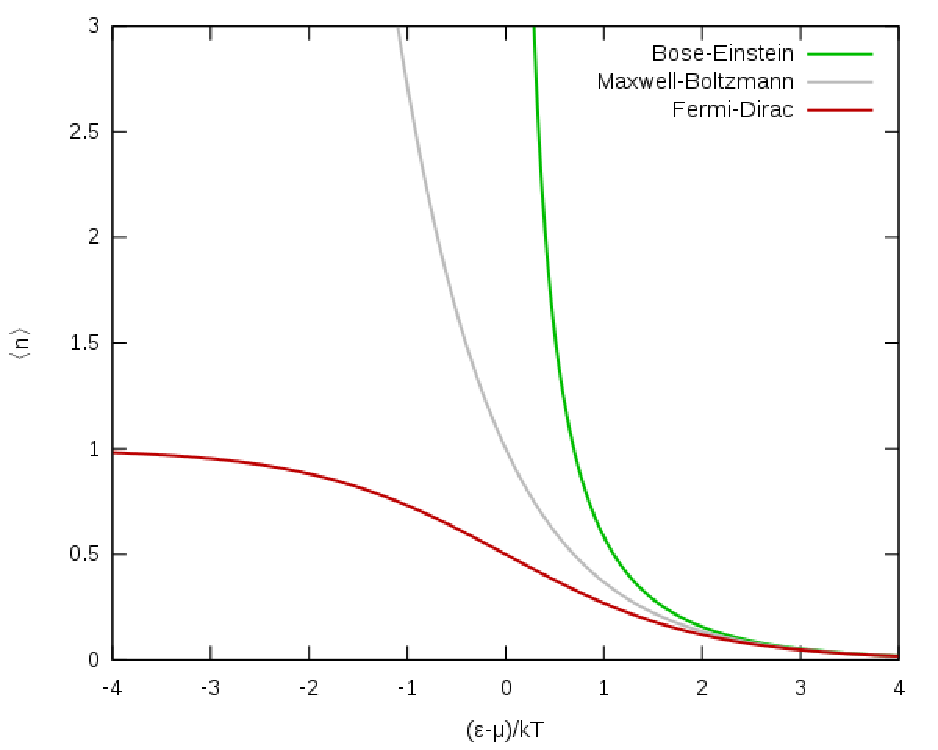
\includegraphics[width=\textwidth]{figs/week07_dist.pdf}\end{center}

In the low-temperature regime $\frac{E_{\ell} - \mu}{T} \ll 1$ corresponding to the left portion of the plot, we see dramatically different behaviour for the three cases.
The classical Maxwell--Boltzmann prediction for the average occupation number grows exponentially, while the quantum Bose--Einstein prediction diverges as $E_{\ell} \to \mu$ and the Fermi--Dirac prediction slowly approaches its maximum possible value $\nFD \to 1$.
Over the next two weeks we will study in more detail the quantum gases of bosons and fermions that produce these results.
% ------------------------------------------------------------------


\newpage
% ------------------------------------------------------------------
\renewcommand{\thisweek}{MATH327 Week 8}
\renewcommand{\moddate}{Last modified 17 Apr.~2021}
\setcounter{section}{8}
\setcounter{subsection}{0}
\phantomsection
\addcontentsline{toc}{section}{Week 8: Quantum gases of bosons}
\section*{Week 8: Quantum gases of bosons}
\subsection{The photon gas}
Last week we derived the grand-canonical partition function (\eq{eq:partfunc_BE}) that defines quantum Bose--Einstein statistics for systems of non-interacting bosons,
\begin{equation*}
  \ZBE(\be, \mu) = \prod_{\ell = 0}^L \frac{1}{1 - e^{-\be (E_{\ell} - \mu)}}.
\end{equation*}
This expression results from summing over the possible occupation numbers $n_{\ell} \in \Nbb_0$ for each energy level $\cE_{\ell}$ with energy $E_{\ell}$.
The corresponding grand-canonical potential is
\begin{equation*}
  \Phi_{\text{BE}} = -T \log Z_g = T \sum_{\ell = 0}^L \log\left[1 - e^{-\be (E_{\ell} - \mu)}\right],
\end{equation*}
from which we can determine the large-scale properties of the system, including its average internal energy $\vev{E}$, average particle number $\vev{N}$, entropy $S$, and pressure $P$.

To do so, we have to specify the energy levels of the particles that compose the system of interest, and the degeneracies of those energy levels.
One example of this that we have already seen is the analysis of non-relativistic ideal gas particles in \secref{sec:regulate}.
For a single particle with mass $m$ in a volume $V = L^3$, we determined the quantized energies
\begin{equation}
  \label{eq:nonrel_energy}
  E(k_x, k_y, k_z) = \frac{\hbar^2 \pi^2}{2mL^2}\left(k_x^2 + k_y^2 + k_z^2\right),
\end{equation}
where the integers $k_{x, y, z}$ specify the possible momenta of the particle,
\begin{align*}
  \vec p & = (p_x, p_y, p_z) = \hbar \frac{\pi}{L} (k_x, k_y, k_z) &
  k_{x, y, z} = 1, 2, \cdots.
\end{align*}
(For technical reasons, quantum mechanics requires $k_{x, y, z} \geq 1$, leading us to adjust our ansatz compared to \eq{eq:quant_mom}.)
This system has a unique ground state $\cE_0$ with $\vec k = (1, 1, 1)$ and energy $E_0 = \frac{3}{2} \frac{\hbar^2 \pi^2}{mL^2}$.
The next three energy levels are degenerate, with energy $3 \frac{\hbar^2 \pi^2}{mL^2}$ corresponding to $\vec k = (2, 1, 1)$ and permutations, followed by another three degenerate energy levels with energy $\frac{9}{2} \frac{\hbar^2 \pi^2}{mL^2}$ corresponding to $\vec k = (2, 2, 1)$ and permutations.

This week we will build on that experience to consider a gas of \textit{photons}, massless bosonic quantum particles of light.
For our purposes, with no prior knowledge of particle physics, we can define photons simply by specifying two relevant details of their energy levels.
First, a photon's energy is proportional to the magnitude of its momentum, %with $m = 0$ for massless photons, \eq{eq:nonrel_energy} is clearly problematic.
\begin{equation*}
  \Eph(p) = c \sqrt{p_x^2 + p_y^2 + p_z^2} \equiv c p.
\end{equation*}
Here the speed of light $c$ is really just a unit conversion factor that we could set to $c = 1$ by using appropriate units.
Second, for each momentum $\vec p$, a photon has two degenerate energy levels with the same energy $E(p)$. % TODO: Could mention polarization...

In a volume $V = L^3$, only the same discrete momenta as above are allowed,
\begin{align*}
  p & = \hbar \frac{\pi}{L} \sqrt{k_x^2 + k_y^2 + k_z^2} \equiv \hbar \frac{\pi}{L} k &
  k_{x, y, z} = 1, 2, \cdots,
\end{align*}
so that the quantized photon energies are
\begin{equation}
  \label{eq:photon_Ek}
  \Eph(k) = \hbar c \frac{\pi}{L} k.
\end{equation}
It is conventional to use the speed of light to work with photons in terms of their wavelength \la and angular frequency $\om = 2\pi f$ (not to be confused with generic micro-states $\om_i$), given the relation
\begin{equation*}
  c = \frac{\la \om}{2\pi}.
\end{equation*}
Just like the momenta, the wavelengths \la are also quantized in volume $V = L^3$,
\begin{equation*}
  \la = \frac{2L}{k} \qquad \Lra \qquad c = \frac{\om}{\frac{\pi}{L} k},
\end{equation*}
and we can rewrite \eq{eq:photon_Ek} as
\begin{equation}
  \label{eq:photon_omega}
  \Eph(\om) = \hbar \om.
\end{equation}
Low (\textit{infrared}) frequencies correspond to small energies and long wavelengths, while high (\textit{ultraviolet}) frequencies correspond to large energies and short wavelengths.

We are now ready to write down the grand-canonical potential for a photon gas:
\begin{equation*}
  \Phi_{\text{ph}} = T \sum_{\ell = 0}^L \log\left[1 - e^{-\be (E_{\ell} - \mu)}\right] = 2T \sum_{\vec k} \log\left[1 - e^{-\be (\Eph(k) - \mu)}\right],
\end{equation*}
where the factor of $2$ in the final expression accounts for the doubly degenerate energy levels.
We can simplify this expression by appreciating that photons are easy to create and destroy.
Every time a light is switched on, it begins emitting a constant flood of photons (with wavelengths of several hundred nanometres).
Food in a microwave oven gets hot by absorbing many lower-energy photons (with longer wavelengths around $12$~centimetres).
In both cases an enormous number of photons is required to make even a small change in energy, so that \eq{eq:mu_E} implies the chemical potential of a photon gas must be negligible,
\begin{equation*}
  \mu = \left.\pderiv{E}{N}\right|_S \approx 0 \qquad \Lra \qquad \Phi_{\text{ph}} \approx 2T \sum_{\vec k} \log\left[1 - e^{-\be \Eph(k)}\right].
\end{equation*}
% TODO: This is a significant simplification, and the reason we only consider photons this week...

Another simplification comes from considering the photon gas in a large volume, so that we can approximate the sum over discrete integer $k_{x, y, z}$ by integrals over continuous real $\khat_{x, y, z}$,
\begin{equation*}
  \Phi_{\text{ph}} \approx 2T \int d\khat_x d\khat_y d\khat_z \log\left[1 - e^{-\be \Eph(\khat)}\right].
\end{equation*}
Since the energy $\Eph(\khat)$ depends only on the magnitude $\khat$, we can profit from converting to spherical coordinates.
When we do so, we have to keep in mind that $k_{x, y, z} > 0$ corresponds only to the positive octant of thee sphere,
\begin{equation*}
  \int_0^{\infty} d\khat_x \int_0^{\infty} d\khat_y \int_0^{\infty} d\khat_z = \int_0^{\infty} d\khat \; \khat^2 \int_0^{\pi / 2} d\theta \; \sin\theta \int_0^{\pi / 2} d\phi = \frac{\pi}{2} \int_0^{\infty} d\khat \; \khat^2,
\end{equation*}
so that
\begin{equation*}
  \Phi_{\text{ph}} \approx \pi T \int_0^{\infty} d\khat \; \khat^2 \log\left[1 - e^{-\be \Eph(\khat)}\right].
\end{equation*}
We can finally change variables to integrate over the photon angular frequency $\om = c \frac{\pi}{L} k$, with $\Eph = \hbar \om$, to find
\begin{align}
  \Phi_{\text{ph}} & \approx \pi T \left(\frac{L}{\pi c}\right)^3 \int_0^{\infty} d\om \; \om^2 \log\left[1 - e^{-\be \hbar \om}\right] \cr
                   & = \frac{VT}{c^3 \pi^2} \int_0^{\infty} d\om \; \om^2 \log\left[1 - e^{-\be \hbar \om}\right], \label{eq:photon_grand}
\end{align}
recognizing $L^3 = V$.
With this grand-canonical potential derived, we just need to take the appropriate derivatives to determine the thermodynamics and equation of state for the photon gas.
% ------------------------------------------------------------------



% ------------------------------------------------------------------
\subsection{The sun and the void}
We are now ready to analyze the average internal energy from the grand-canonical potential for a photon gas, \eq{eq:photon_grand}.
With $\mu = 0$, \eq{eq:E_grand} from week~6 becomes
\begin{equation*}
  \vev{E}_{\text{ph}} = -T^2 \pderiv{}{T} \left[\frac{\Phi_{\text{ph}}}{T}\right] = \pderiv{}{\be} \left[\be \Phi_{\text{ph}}\right].
\end{equation*}
To begin, we will consider the energy density expressed as an integral over photon frequencies,
\begin{equation*}
  \frac{\vev{E}_{\text{ph}}}{V} = \int_0^{\infty} P(\om) \; d\om,
\end{equation*}
where the function $P(\om)$ is known as the \textit{spectral density}, or simply the \textit{spectrum}.
What is the spectrum for a photon gas?
\begin{mdframed}
  $\displaystyle \frac{\vev{E}_{\text{ph}}}{V} = \frac{1}{c^3 \pi^2} \int_0^{\infty} d\om \; \om^2 \pderiv{}{\be} \log\left[1 - e^{-\be \hbar \om}\right] = $ \\[100 pt]
\end{mdframed}

You should find
\begin{equation}
  \label{eq:Planck_omega}
  P(\om) = \left(\frac{\hbar}{c^3 \pi^2}\right) \frac{\om^3}{e^{\be \hbar \om} - 1},
\end{equation}
which is known as the Planck spectrum, named after Max Planck.
The Planck spectrum is plotted in the figure below, which comes from \href{https://commons.wikimedia.org/wiki/File:Black_body.svg}{Wikimedia Commons}.

\begin{center}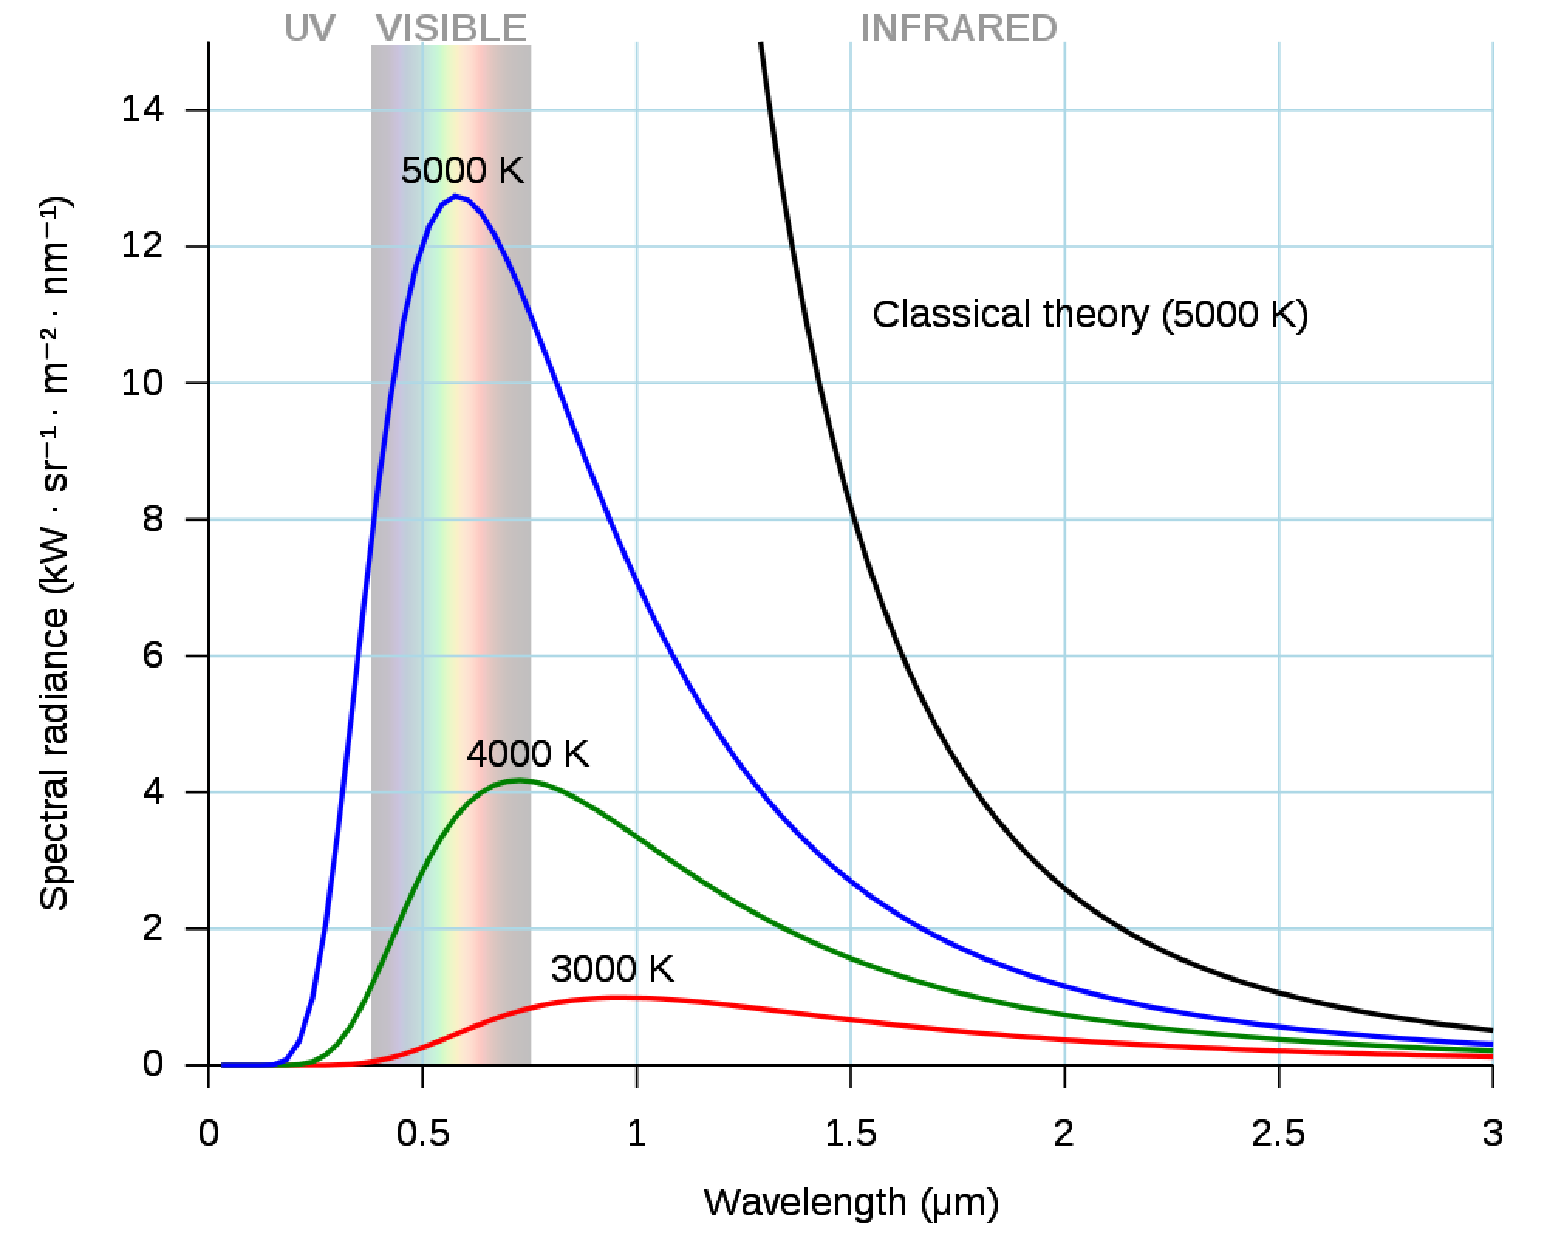
\includegraphics[width=\textwidth]{figs/week08_spectrum.pdf}\end{center}

In this plot the horizontal axis uses the wavelength $\la = 2\pi c / \om$.
Changing variables in your work above, what is Planck spectrum $P(\la)$ as a function of wavelength?
\begin{mdframed}
  $\displaystyle \frac{\vev{E}_{\text{ph}}}{V} = \frac{\hbar}{c^3 \pi^2} \int_0^{\infty} \frac{\om^3}{e^{\be \hbar \om} - 1} \; d\om = $ \\[120 pt] % WARNING: FORMATTING BY HAND
\end{mdframed}

You should find
\begin{equation}
  \label{eq:Planck_la}
  P(\la) = \left(\frac{16\pi^2 \hbar c}{\la^5}\right) \frac{1}{e^{2\pi\be \hbar c / \la} - 1},
\end{equation}
which is plotted\footnote{The plot divides our $P(\la)$ by $4\pi$~steradian and multiplies it by $c$ to convert from an energy density to a spectral power per unit area per unit of solid angle.  For our purposes only the functional form is significant.} for three temperatures $T = 1 / \be$ in the figure above.
Considering first the high-energy ultraviolet (UV) limit of small wavelengths $\la$, we can see from \eq{eq:Planck_la} that $P(\la)$ is exponentially suppressed, which overwhelms the diverging factor $\propto 1 / \la^5$ in parentheses.

In the low-energy infrared limit, the large $\la$ has the same effect that a large temperature ($\be \ll 1$) would have: $e^{2\pi\be \hbar c / \la} - 1 \approx 2\pi\be \hbar c / \la$ and
\begin{equation*}
  P(\la) \approx \left(\frac{16\pi^2 \hbar c}{\la^5}\right) \frac{\la}{2\pi\be \hbar c} = \frac{8\pi T}{\la^4}.
\end{equation*}
The connection to large temperatures indicates that this is what classical statistics would predict for the energy spectrum of light.
It is known as the Rayleigh--Jeans spectrum, named after \href{https://en.wikipedia.org/wiki/John_William_Strutt,_3rd_Baron_Rayleigh}{the third Baron Rayleigh} and \href{https://en.wikipedia.org/wiki/James_Jeans}{James Jeans}.
Recall that the classical approach sums over all possible energies for each degree of freedom, corresponding to a light-emitting object (historically known as a \textit{black body}) emitting light of all wavelengths $\la$.
According to the classical Rayleigh--Jeans spectrum, in the limit $\la \to 0$ this light would carry an infinite amount of energy, an obvious error that became known as the \textit{ultraviolet catastrophe}.
Planck's (heuristic) solution to this conundrum in 1900 was one of the first steps towards the quantum physics that introduces the exponential suppression we computed above.

One final observation we will make about the Planck spectrum shown above is that as the temperature increases, the maximum of the Planck spectrum moves to shorter wavelengths and correspondingly larger energies.
The fact that the peak of the spectrum for $T \approx 5000$~K falls within the wavelengths of visible light (roughly $400$--$700$~nm) is not a coincidence.
As shown in the figure below (from \href{https://commons.wikimedia.org/wiki/File:Solar_Spectrum.png}{Wikimedia Commons}), the amount of sunlight that reaches the surface of the earth is also maximized around visible wavelengths, which are visible to us because we have evolved to make the most efficient use of this sunlight.

Taking into account the absorption of some sunlight by molecules in the atmosphere, we can see from the figure below that the energy spectrum of the sunlight reaching the top of the atmosphere is quite close to a Planck (or `blackbody') spectrum with temperature $T \approx 5778$~K.
The agreement isn't perfect, which is to be expected since the Planck spectrum relies on the non-trivial assumption of an ideal gas of non-interacting particles.
Even with that caveat, numerically fitting the measured sunlight to the Planck spectrum is how the surface temperature of the sun is determined to be $T \approx 5778$~K.
This same fitting procedure can even be done for distant stars, with red stars corresponding to relatively low temperatures $T \lesssim 3500$~K and blue stars corresponding to relatively high temperatures $T \gtrsim 10{,}000$~K.

\begin{center}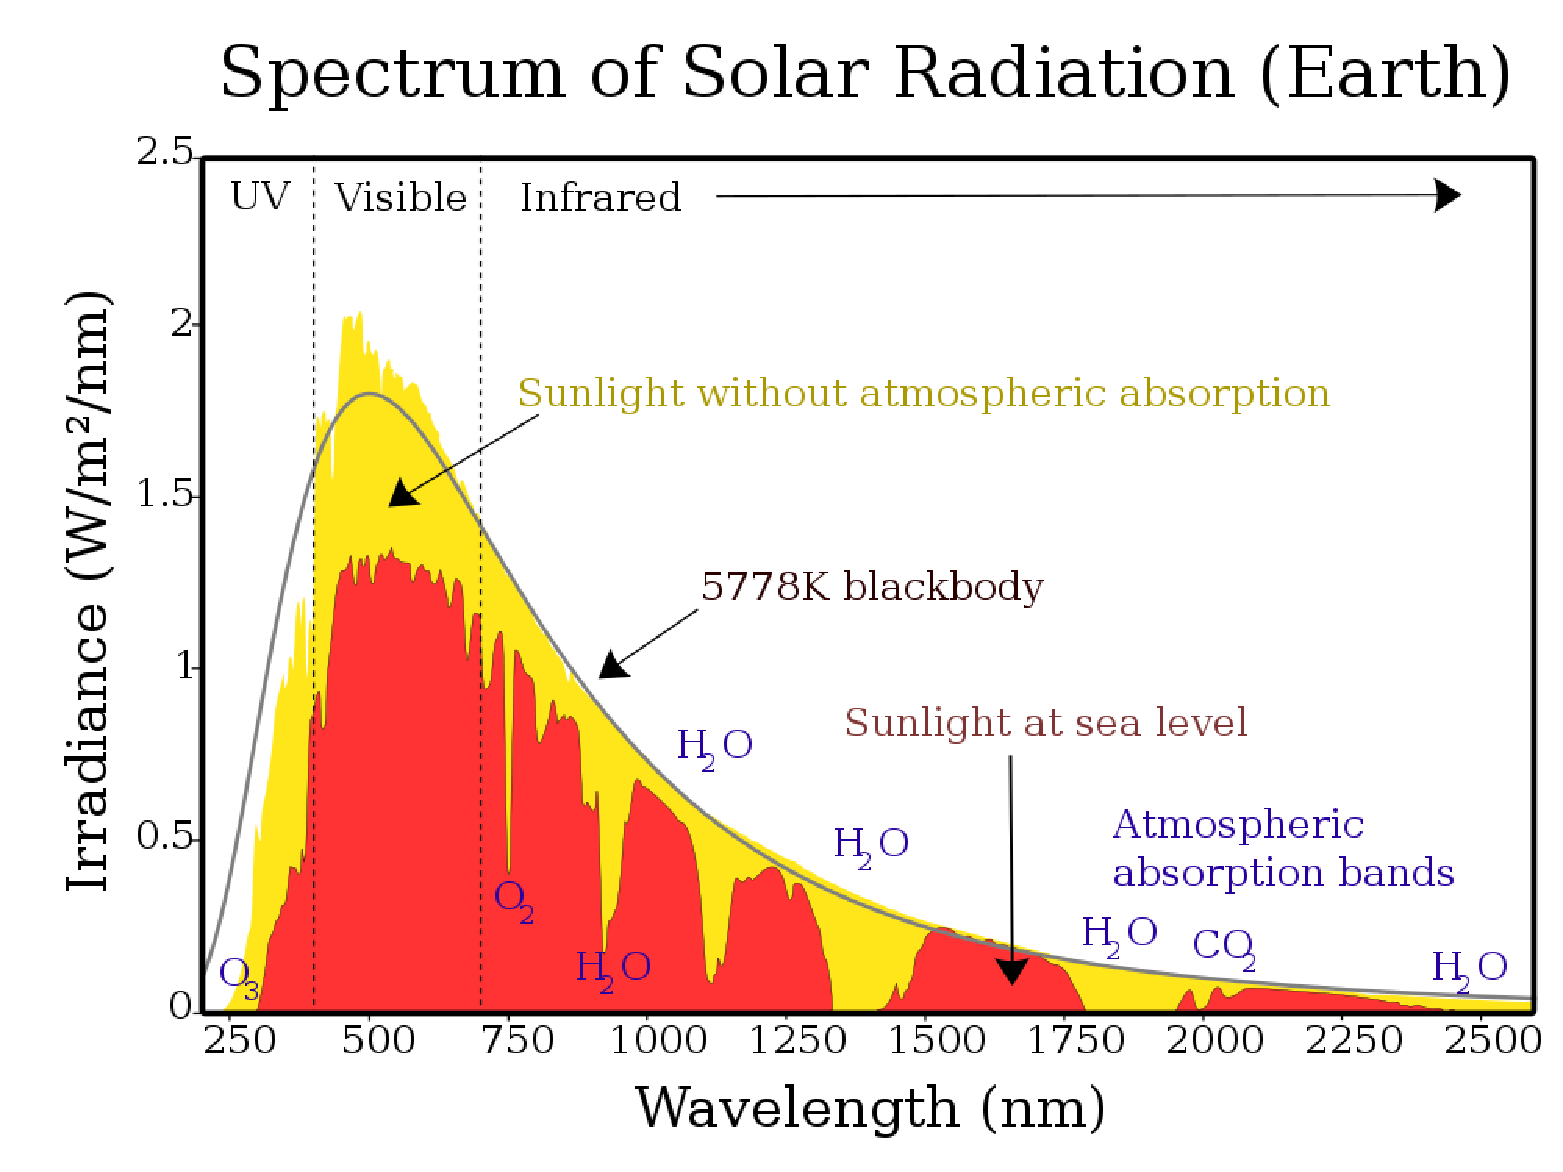
\includegraphics[width=\textwidth]{figs/week08_sun.pdf}\end{center}

In fact, we can even use the Planck spectrum to determine the temperature of inter-galactic space.
Rather than being empty, these voids are actually permeated by a very low-temperature photon gas left over from the Big Bang roughly $14$~billion years ago.
This photon gas is known as the \href{https://en.wikipedia.org/wiki/Cosmic_microwave_background}{cosmic microwave background} (CMB), and carries information about the early evolution of the universe, including some of the strongest evidence for the existence of dark matter.

The picture below is a famous visualization of the CMB, provided by the \href{http://www.esa.int/ESA_Multimedia/Images/2013/03/Planck_CMB}{European Space Agency} and produced from measurements taken by their `Planck' satellite. % Can compare with WMAP from wmap.gsfc.nasa.gov/media/101080/
To produce this image, for each point in the sky the satellite measures the photon spectrum reaching it from that direction.
The contributions coming from stars and galaxies are subtracted, and the remaining data is fit to the Planck spectrum to find the temperature of the intergalactic CMB photon gas at that point.
From point to point, there are only small temperature fluctuations around the average $T_{\text{CMB}} \approx 2.725$~K.
That average temperature is subtracted and the fluctuations themselves are shown below, with warmer red-coloured regions only $\De T \approx 0.0002$~K hotter than the cooler blue-coloured regions.

\begin{center}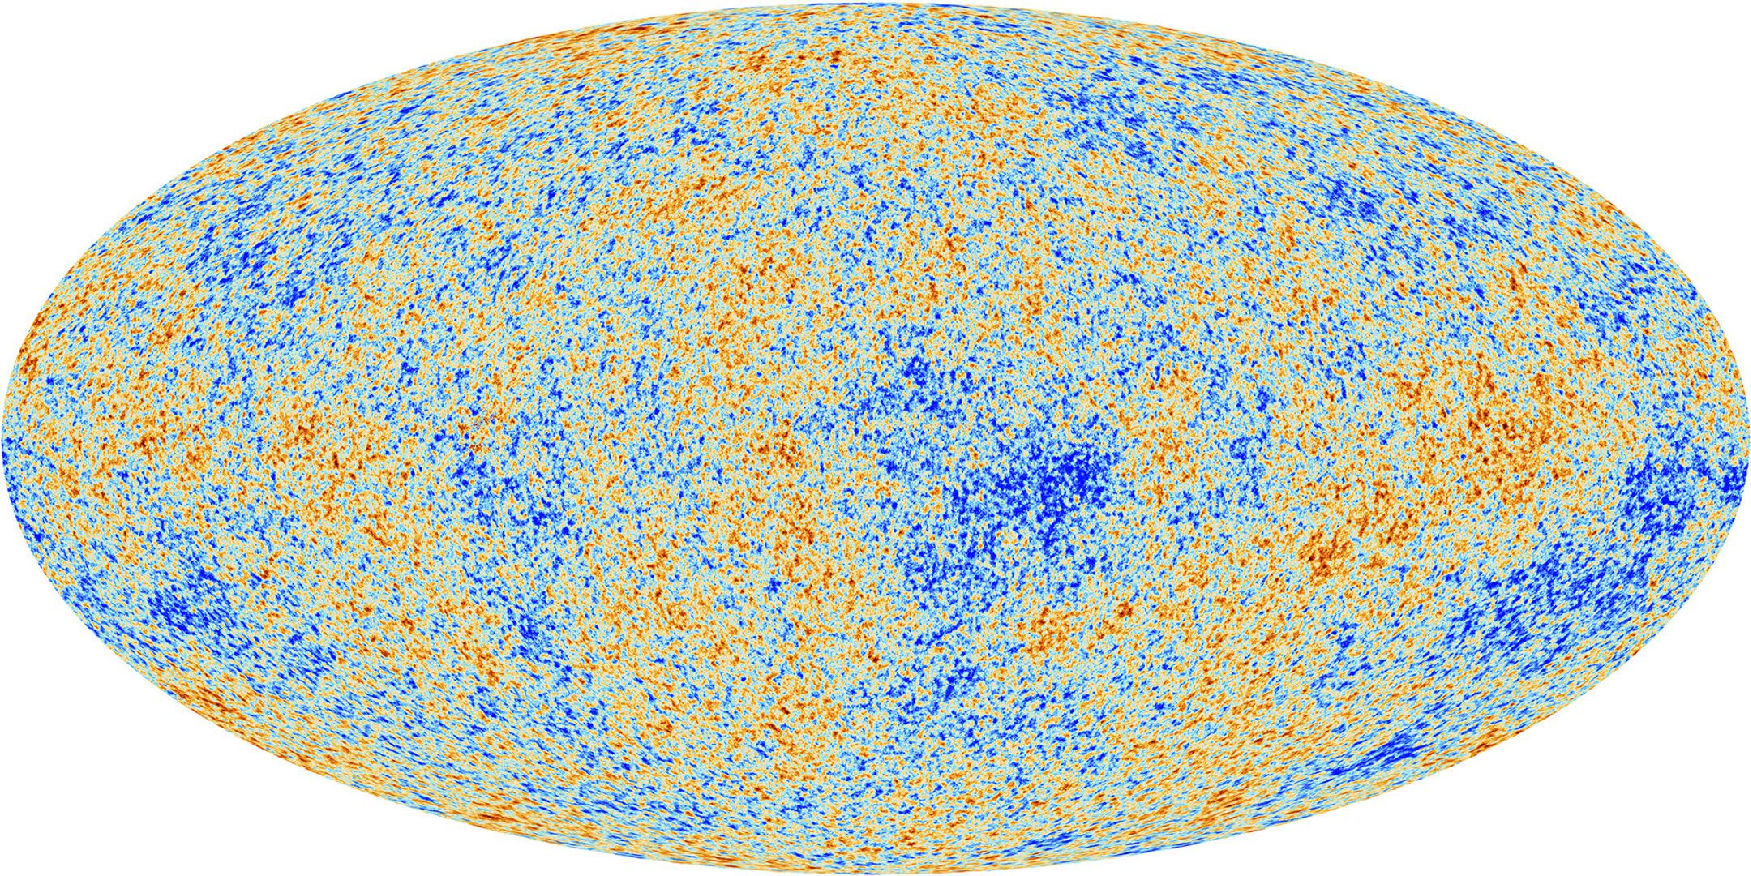
\includegraphics[width=\textwidth]{figs/week08_CMB.pdf}\end{center}

The final figure below illustrates such a fit of CMB data to the Planck spectrum, using measurements taken by the Cosmic Background Explorer (COBE) satellite and \href{https://doi.org/10.1086/185717}{published in 1990}.
(This version of the figure is adapted from that publication, and copied from Schroeder's \textit{Introduction to Thermal Physics}.)
The squares are the measured data, and their size represents a cautious estimate of uncertainties.
They are plotted with the frequency $f = \om / (2\pi)$ on the horizontal axis, with $f \approx 3\cdot 10^{-11}~\text{s}^{-1}$ corresponding to a low-energy wavelength $\la = c / f \approx 1$~mm, roughly $1000$ times longer than the wavelengths of visible light.
The solid line is a fit to the data that produces $T_{\text{CMB}} = 2.735 \pm 0.060$~K.
While more recent satellites have increased the precision with which we know $T_{\text{CMB}}$, this first result was awarded the 2006 Nobel Prize in Physics.

\begin{center}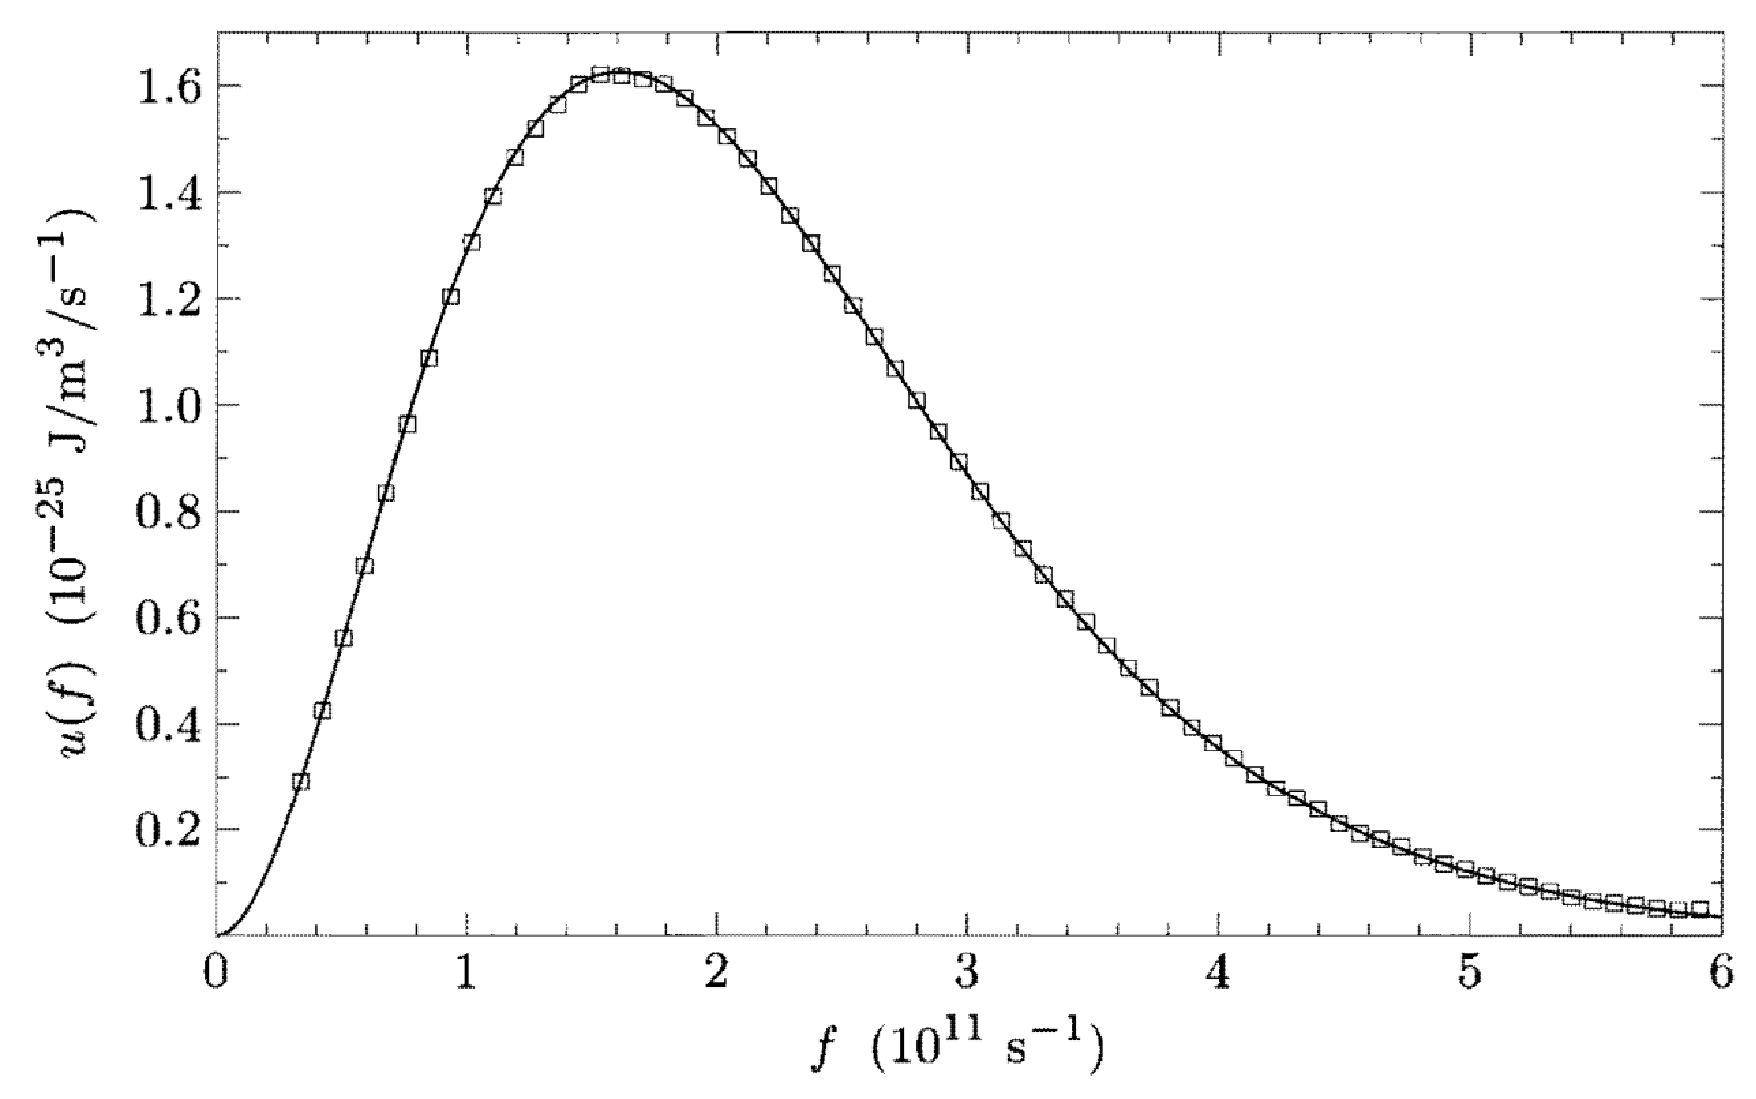
\includegraphics[width=\textwidth]{figs/week08_COBE.pdf}\end{center}

\begin{shaded}
  Even though we derived the Planck spectrum by assuming an ideal gas of non-interacting photons, we see that it provides an excellent mathematical model for real physical systems, stretching from the hottest to the coldest places in the universe.
\end{shaded}
% ------------------------------------------------------------------



% ------------------------------------------------------------------
\subsection{Equation of state for the photon gas}
Having looked in some detail at the integrand for the photon gas energy density, \eq{eq:Planck_omega}, let's complete the integration, which involves a famous integral related to the Riemann zeta function:
\begin{equation*}
  I_4 = \int_0^{\infty} \frac{x^3}{e^x - 1} dx = \Gamma(4) \zeta(4) = \frac{\pi^4}{15}.
\end{equation*}
Using this result, what is the ideal photon gas energy density?
\begin{mdframed}
  $\displaystyle \frac{\vev{E}_{\text{ph}}}{V} = \frac{\hbar}{c^3 \pi^2} \int_0^{\infty} \frac{\om^3}{e^{\be \hbar \om} - 1} \; d\om = $ \\[100 pt]
\end{mdframed}

You should find a result proportional to $T^4$.
It would be ideal (sorry) if we could put this in a form as simple as \eq{eq:ideal_energy} for the energy of an $N$-particle non-relativistic ideal gas in the canonical ensemble.
Now that we are working in the grand-canonical ensemble, this requires computing the average photon number from \eq{eq:N_grand},
\begin{equation*}
  \vev{N}_{\text{ph}} = -\left. \pderiv{}{\mu} \Phi_{\text{ph}}\right|_{\mu = 0} = -\left. \frac{VT}{c^3 \pi^2} \int_0^{\infty} d\om \; \om^2 \pderiv{}{\mu} \log\left[1 - e^{-\be \hbar \om} e^{\be \mu}\right] \right|_{\mu = 0}.
\end{equation*}
recalling $\mu = 0$ for photon gases.
The calculation is quite similar to that for the average internal energy density, now involving the integral
\begin{equation*}
  I_3 = \int_0^{\infty} \frac{x^2}{e^x - 1} dx = \Gamma(3) \zeta(3) = 2\zeta(3).
\end{equation*}
\newpage % WARNING: FORMATTING BY HAND
\noindent Using this result, what is the ideal photon gas number density?
\begin{mdframed}
  $\displaystyle \frac{\vev{N}_{\text{ph}}}{V} = \frac{1}{c^3 \pi^2} \int_0^{\infty} \frac{\om^2}{e^{\be \hbar \om} - 1} \; d\om = $ \\[100 pt]
\end{mdframed}

You should find a result proportional to $T^3 \propto \vev{E}_{\text{ph}} / T$, so that
\begin{equation}
  \vev{E}_{\text{ph}} = \frac{\pi^2}{15 \hbar^3 c^3} VT^4 = \frac{\pi^4}{30\zeta(3)} \vev{N}_{\text{ph}} T.
\end{equation}
The functional form is the same as \eq{eq:ideal_energy}, with a larger numerical factor
\begin{equation*}
  \frac{\pi^4}{30\zeta(3)} = \frac{\Gamma(4) \zeta(4)}{\Gamma(3) \zeta(3)} \approx 2.7
\end{equation*}
compared to the $\frac{3}{2}$ for the classical non-relativistic case.

To get the rest of the way to the equation of state for the photon gas, we need to compute the \textit{radiation pressure}
\begin{equation*}
  P_{\text{ph}} = -\left. \pderiv{}{V} \vev{E}_{\text{ph}} \right|_{S_{\text{ph}}},
\end{equation*}
which requires first figuring out the condition of constant entropy $S_{\text{ph}}$ for a photon gas.
From \eq{eq:grand_relation} with $\mu = 0$, we have
\begin{equation*}
  S_{\text{ph}} = \frac{\vev{E}_{\text{ph}} - \Phi_{\text{ph}}}{T}.
\end{equation*}
Looking back to \eq{eq:photon_grand} for the grand-canonical potential, we see
\begin{equation*}
  \frac{\Phi_{\text{ph}}}{T} = \frac{V}{c^3 \pi^2} \int_0^{\infty} d\om \; \om^2 \log\left[1 - e^{-\be \hbar \om}\right] = \frac{VT^3}{\hbar^3 c^3 \pi^2} \int_0^{\infty} dx \; x^2 \log\left[1 - e^{-x}\right],
\end{equation*}
changing variables to $x = \be \hbar \om = \hbar \om / T$.
The final factor in this expression is yet another delightful integral,
\begin{equation*}
  \int_0^{\infty} dx \; x^2 \log\left[1 - e^{-x}\right] = -2\zeta(4) = -\frac{\pi^4}{45}.
\end{equation*}
Since this gives us $S \propto VT^3$, we can conclude that the condition of constant entropy for a photon gas is $V T^3 = \mbox{constant}$, in contrast to the $V T^{3/2}$ dependence of \eq{eq:ideal_entropy} for classical non-relativistic particles.

\newpage % WARNING: FORMATTING BY HAND
At this point we just need to insert the constant-entropy condition $T = b V^{-1 / 3}$ (with $b$ a constant) into the average internal energy and take the derivative:
\begin{mdframed}
  $\displaystyle P = -\left. \pderiv{}{V} \vev{E}_{\text{ph}} \right|_{S_{\text{ph}}} = -\pderiv{}{V} \frac{\pi^2}{15 \hbar^3 c^3} b^4 V^{-1 / 3} = $ \\[100 pt]
\end{mdframed}
You should find the following equation of state for the photon gas,
\begin{equation}
  P_{\text{ph}} V = \frac{1}{3} \vev{E}_{\text{ph}} = \frac{\pi^4}{90\zeta(3)} \vev{N}_{\text{ph}} T.
\end{equation}
The functional form is the same as the (classical, non-relativistic) ideal gas law, with just an additional numerical factor
\begin{equation*}
  \frac{\pi^4}{90\zeta(3)} = \frac{\zeta(4)}{\zeta(3)}.
\end{equation*}
% ------------------------------------------------------------------


\newpage
% ------------------------------------------------------------------
\renewcommand{\thisweek}{MATH327 Week 9}
\renewcommand{\moddate}{Last modified 24 Apr.~2021}
\setcounter{section}{9}
\setcounter{subsection}{0}
\phantomsection
\addcontentsline{toc}{section}{Week 9: Quantum gases of fermions}
\section*{Week 9: Quantum gases of fermions}
\subsection{\label{sec:fermi_nonrel}Non-relativistic ideal fermion gas}
This week we wrap up our applications of the grand-canonical ensemble to investigate ideal gases of non-interacting particles.
We again take the quantum statistical approach of defining micro-states by summing over the possible occupation numbers $n_{\ell}$ for each energy level $\cE_{\ell}$ with energy $E_{\ell}$.
In contrast to the bosonic case considered last week, we now focus on quantum gases of fermions, where the only possible occupation numbers are $n_{\ell} = 0$ and $1$, since the Pauli exclusion principle prevents multiple identical fermions from occupying the same energy level.

In \secref{sec:fermi} we derived the grand-canonical partition function (\eq{eq:partfunc_FD}) that defines quantum Fermi--Dirac statistics for such systems of non-interacting fermions,
\begin{equation*}
  \ZFD(\be, \mu) = \prod_{\ell = 0}^L \left[1 + e^{-\be (E_{\ell} - \mu)}\right],
\end{equation*}
for inverse temperature $\be = 1 / T$ and chemical potential $\mu$.
Recall that it is possible for systems of fermions to have any value for the chemical potential (either positive or negative), in contrast to the systems of bosons we considered last week.
From the corresponding grand-canonical potential,
\begin{equation*}
  \Phi_{\text{FD}} = -T \sum_{\ell = 0}^L \log\left[1 + e^{-\be (E_{\ell} - \mu)}\right]
\end{equation*}
we can determine the large-scale properties of the system, including its average internal energy $\vev{E}$, average particle number $\vev{N}$, entropy $S$, and pressure $P$, along with the equation of state relating these quantities.

A concrete calculation requires specifying the energy levels of the particles that compose the gas, and the degeneracies of those energy levels.
Let's begin this week by considering non-relativistic particles of the sort we previously analyzed in \secref{sec:regulate}.
In a volume $V = L^3$, the energy levels are defined by the non-zero quantized energies
\begin{align*}
  E(k) & = \frac{p^2}{2m} = \frac{\hbar^2 \pi^2}{2mL^2}\left(k_x^2 + k_y^2 + k_z^2\right) &
  k_{x, y, z} & = 1, 2, \cdots.
\end{align*}
In addition to the usual degeneracies coming from permutations of $(k_x, k_y, k_z)$ that we discussed in previous weeks, for each distinct $\vec k$ typical fermions such as electrons have two degenerate energy levels with the same energy.
This factor of $2$ has a different origin compared to the double degeneracy discussed for photons last week.
Rather than worry about the physical origins of this behaviour, in both cases we simply incorporate this given information into our ansatz. % TODO: Could mention spin...

The grand-canonical potential for an ideal gas of non-relativistic fermions is therefore
\begin{equation*}
  \Phi_{\text{f}} = T \sum_{\ell = 0}^L \log\left[1 + e^{-\be (E_{\ell} - \mu)}\right] = 2T \sum_{\vec k} \log\left[1 + \exp\left(-\frac{\hbar^2 \pi^2 k^2}{2mL^2 T} + \frac{\mu}{T}\right)\right].
\end{equation*}
We can again proceed by considering the gas in a large volume and approximating the sum over discrete integer $k_{x, y, z}$ by integrals over continuous real $\khat_{x, y, z}$:
\begin{equation*}
  \Phi_{\text{f}} \approx 2T \int d\khat_x d\khat_y d\khat_z \log\left[1 + \exp\left(-\frac{\hbar^2 \pi^2 \khat^2}{2mL^2 T} + \frac{\mu}{T}\right)\right].
\end{equation*}
Converting to spherical coordinates and carrying out the angular integrations over the $\frac{\pi}{2}$ solid angle of the octant of the sphere with $k_{x, y, z} > 0$, we have
\begin{equation*}
  \Phi_{\text{f}} \approx \pi T \int_0^{\infty} d\khat \; \khat^2 \log\left[1 + \exp\left(-\frac{\hbar^2 \pi^2 \khat^2}{2mL^2 T} + \frac{\mu}{T}\right)\right].
\end{equation*}
In the same spirit as the change of variables we carried out last week, to integrate over photon frequencies $\om = \Eph / \hbar$, we will now change variables to integrate over the fermion energy:
\begin{align*}
  E = \frac{\hbar^2 \pi^2}{2mL^2}\khat^2 \quad \lra \quad \khat & = \frac{L\sqrt{m}}{\pi \hbar} \sqrt{2E} \cr
                                                         d\khat & = \frac{L\sqrt{m}}{\pi \hbar} \frac{dE}{\sqrt{2E}}.
\end{align*}
Plugging this in produces
\begin{align}
  \Phi_{\text{f}} & \approx \pi T \left(\frac{L^3 m^{3 / 2}}{\pi^3 \hbar^3}\right) \int_0^{\infty} dE \frac{2E}{\sqrt{2E}} \log\left[1 + e^{-\be(E - \mu)}\right] \cr
                  & = \frac{\sqrt{2 m^3} VT}{\pi^2 \hbar^3} \int_0^{\infty} dE \sqrt{E} \log\left[1 + e^{-\be(E - \mu)}\right]. \label{eq:fermi_grand}
\end{align}
recognizing $L^3 = V$.

With this grand-canonical potential derived, we just need to take the appropriate derivatives to determine the thermodynamics and equation of state for non-relativistic fermions.
When doing so, we'll focus on the low-temperature regime where we expect quantum Fermi--Dirac statistics to differ significantly from the classical case we considered back in \secref{sec:regulate}.
As we saw in \secref{sec:quantum_classical}, at high temperatures (with large negative chemical potential) the classical approach provides a good approximation to the true quantum physics.
% TODO: Low temperatures provide a significant simplification, which is why we only consider that regime this week
% ------------------------------------------------------------------



% ------------------------------------------------------------------
\subsection{Low-temperature equation of state}
Rather than the average internal energy $\vev{E}_{\text{f}}$, it will prove profitable to first analyze the average particle number
\begin{equation*}
  \vev{N}_{\text{f}} = -\pderiv{}{\mu} \Phi_{\text{f}}
\end{equation*}
coming from the grand-canonical potential for non-relativistic fermions, \eq{eq:fermi_grand}.
In analogy to the Planck spectrum we derived for the photon gas last week, we first express the particle number density as an integral over energies,
\begin{equation*}
  \frac{\vev{N}_{\text{f}}}{V} = \frac{\sqrt{2m^3}}{\pi^2 \hbar^3} \int_0^{\infty} F(E) \sqrt{E} \; dE,
\end{equation*}
where the function $F(E)$ is known as the Fermi function.
In contrast to the Planck spectrum, all the constant factors are kept separate from $F(E)$:
\begin{align}
  \frac{\vev{N}_{\text{f}}}{V} & = \frac{\sqrt{2m^3} T}{\pi^2 \hbar^3} \int_0^{\infty} dE \sqrt{E} \pderiv{}{\mu} \log\left[1 + e^{-\be(E - \mu)}\right] \cr
                               & = \frac{\sqrt{2m^3}}{\pi^2 \hbar^3} \int_0^{\infty} \frac{1}{e^{\be(E - \mu)} + 1} \sqrt{E} \; dE = \frac{\sqrt{2m^3}}{\pi^2 \hbar^3} \int_0^{\infty} F(E) \sqrt{E} \; dE. \label{eq:N_fermi}
\end{align}
This allows the Fermi function to closely resemble the average occupation numbers $\vev{n_{\ell}}$ we computed in \secref{sec:quantum_classical}:
\begin{equation}
  F(E) = \frac{1}{e^{\be(E - \mu)} + 1}.
\end{equation}

As usual in the grand-canonical approach, the average particle number and Fermi function depend on both the inverse temperature \be and the chemical potential $\mu$.
Expressing $F(E)$ in terms of the dimensionless ratios $E / \mu$ and $T / \mu$,
\begin{equation*}
  F(E) = \frac{1}{\exp\left[\frac{E - \mu}{T}\right] + 1} = \frac{1}{\exp\left[\frac{\mu}{T}\left(\frac{E}{\mu} - 1\right)\right] + 1} = \frac{1}{\left(\exp\left[\frac{E}{\mu} - 1\right]\right)^{\mu / T} + 1},
\end{equation*}
we can highlight the two main features of the figure below, which plots the Fermi function against $E / \mu$ for various temperatures $T / \mu$.

\begin{center}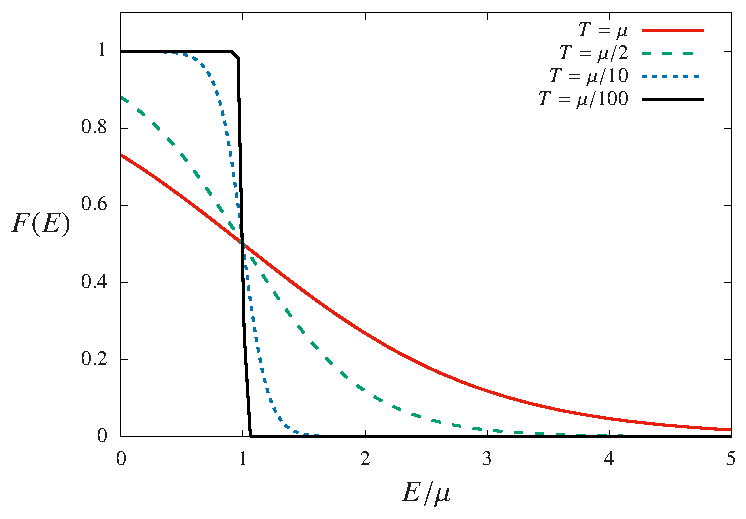
\includegraphics[width=\textwidth]{figs/week09_dist.pdf}\end{center}

First, we can see that the point $E = \mu$, where $F(E) = 1 / 2$ for any non-zero temperature, is a threshold at which the behaviour of the Fermi function changes.
For larger energies $E > \mu$, the exponential factor $\exp\left[\frac{E}{\mu} - 1\right] > 1$ and drives $F(E) \to 0$ as the energy increases.
For smaller energies $E < \mu$, the exponential factor $\exp\left[\frac{E}{\mu} - 1\right] < 1$ and vanishes as the energy decreases, leaving $F(E) \to 1$.
These two asymptotic limits reflect the possible energy level occupation numbers for fermions, $n_{\ell} = 0$ and $1$.
Second, smaller temperatures cause much more rapid approach to these two limits, with the exponential factor either enhanced (if $E > \mu$) or suppressed (if $E < \mu$) by a power $\mu / T \gg 1$.
Therefore, for small temperatures $T \ll \mu$, we can simplify our calculations by approximating the Fermi function as a step function,
\begin{equation}
  \label{eq:Fermi_step}
  F(E) \approx \left\{\begin{array}{l}1 \qquad \mbox{for } \ E < \mu \\
                                      0 \qquad \mbox{otherwise}\end{array}\right. .
\end{equation}
Using this approximation, what is the resulting particle number density?
\begin{mdframed}
  $\displaystyle \frac{\vev{N}_{\text{f}}}{V} = \frac{\sqrt{2m^3}}{\pi^2 \hbar^3} \int_0^{\infty} F(E) \sqrt{E} \; dE = $ \\[100 pt]
\end{mdframed}

You should find a result proportional to $\mu^{3 / 2}$ but independent of $T$.
The temperature independence can be understood by viewing this as the leading-order term in an expansion in the small temperature (known as a \textit{Sommerfeld expansion}, named after \href{https://en.wikipedia.org/wiki/Arnold_Sommerfeld}{Arnold Sommerfeld}).
The $\mu^{3 / 2}$ dependence on the chemical potential is also what we would predict even without doing the detailed calculation.
The step function in \eq{eq:Fermi_step} corresponds to a single fermion occupying each and every energy level with $E_{\ell} < \mu$, while all energy levels with $E_{\ell} > \mu$ are unoccupied.
Since $E(k) \propto k^2$, summing over all $k_{x, y, z}$ corresponds to computing (a portion of) the volume of a sphere of radius $r = \sqrt{\mu}$, which is proportional to $r^3 = \mu^{3 / 2}$ as we found directly above.
If we were to invert this relation, we would obtain the so-called \textbf{Fermi energy} as a function of the particle number density,
\begin{equation}
  \label{eq:Fermi_energy}
  E_F = \mu = \frac{\hbar^2}{2m}\left(\frac{3\pi^2 \vev{N}_{\text{f}}}{V}\right)^{2 / 3}.
\end{equation}

Now we can consider the average energy density of the non-relativistic fermion gas at low temperatures.
Rather than taking another derivative of the grand-canonical potential, we can note from \eq{eq:total_energy_levels} and from our work on the photon gas last week that
\begin{equation}
  \frac{\vev{E}_{\text{f}}}{V} = \frac{\sqrt{2m^3}}{\pi^2 \hbar^3} \int_0^{\infty} E \; F(E) \sqrt{E} \; dE.
\end{equation}
That is, instead of simply counting the number of fermions in the system, we need to add up their energies, introducing an extra factor of $E$ compared to \eq{eq:N_fermi}.
Still using the low-temperature step-function approximation for the Fermi function in \eq{eq:Fermi_step}, what is the average energy density?
\begin{mdframed}
  $\displaystyle \frac{\vev{E}_{\text{f}}}{V} = \frac{\sqrt{2m^3}}{\pi^2 \hbar^3} \int_0^{\infty} F(E) E^{3 / 2} \; dE = $ \\[100 pt]
\end{mdframed}

You should find
\begin{equation}
  \label{eq:fermi_E_N}
  \vev{E}_{\text{f}} = \frac{3}{5} \mu \vev{N}_{\text{f}},
\end{equation}
which means that the average energy of the fermions in a low-temperature ideal gas is $3 / 5$ the Fermi energy $E_F = \mu$.
In particular, because this result is also independent of the temperature, we find that non-interacting quantum fermions retain a positive energy even as the temperature approaches absolute zero, $T \to 0$.
This can be understood by recalling that the lowest-energy pair of degenerate energy levels can each only hold a single fermion, forcing all additional fermions to `fill' energy levels with larger energies $E_{\ell} > 0$, up to the Fermi energy set by the chemical potential.
This is a stark contrast to the classical ($\vev{E} \propto T$) and bosonic ($\vev{E} \propto T^4$) cases we considered earlier, where the average energy vanishes in the zero-temperature limit.
As discussed in Sections~\ref{sec:spin_info} and \ref{sec:quantum_classical}, in those cases all the particles in the system are able to fall into the lowest energy level, with only an exponentially small probability for particles to occupy any energy levels with $E_{\ell} > E_0$.

To get the rest of the way to the equation of state for the ideal gas of non-relativistic fermions, we need to compute the pressure
\begin{equation*}
  P_{\text{f}} = -\left. \pderiv{}{V} \vev{E}_{\text{f}} \right|_{N, S_{\text{f}}}.
\end{equation*}
In the low-temperature limit, the condition of constant entropy $S_{\text{f}} = -\sum_{i = 1}^M p_i \log p_i$ is automatically satisfied, since the step function in \eq{eq:Fermi_step} restricts the system to a single micro-state, resulting in $S_{\text{f}} = 0$.
This micro-state is the one in which each and every energy level with $E_{\ell} < \mu$ is occupied, while all energy levels with $E_{\ell} > \mu$ are unoccupied.

Inserting \eq{eq:Fermi_energy} into \eq{eq:fermi_E_N}, we have
\begin{equation*}
  \vev{E}_{\text{f}} = \frac{3}{5} \mu \vev{N}_{\text{f}} = \frac{3}{5} \left(\frac{\hbar^2}{2m}\right) \left(\frac{3\pi^2}{V}\right)^{2 / 3} \vev{N}_{\text{f}}^{5 / 3}.
\end{equation*}
The pressure is therefore
\begin{align}
  P_{\text{f}} & = -\pderiv{}{V} \left[\frac{3}{5} \left(\frac{\hbar^2}{2m}\right) \left(\frac{3\pi^2}{V}\right)^{2 / 3} \vev{N}_{\text{f}}^{5 / 3}\right] = \frac{2}{3V} \left[\frac{3}{5} \left(\frac{\hbar^2}{2m}\right) \left(\frac{3\pi^2}{V}\right)^{2 / 3} \vev{N}_{\text{f}}^{5 / 3}\right] \nonumber \\
               & = \left(3\pi^2\right)^{2 / 3} \frac{\hbar^2}{5m} \left(\frac{\vev{N}_{\text{f}}}{V}\right)^{5 / 3} = \frac{2}{5} \mu \frac{\vev{N}_{\text{f}}}{V} = \frac{2}{3} \frac{\vev{E}_{\text{f}}}{V}.
\end{align}
The three expressions in the second line above present several relations between the pressure, the energy density, the Fermi energy $E_F = \mu$ and the particle number density.
In particular, we can see that the pressure (like the energy) remains positive even as the temperature approaches absolute zero, with
\begin{equation}
  \label{eq:degen_pressure}
  P_{\text{f}} = \left(3\pi^2\right)^{2 / 3} \frac{\hbar^2}{5m} \rho_{\text{f}}^{5 / 3},
\end{equation}
where we define the density $\rho_{\text{f}} = \vev{N}_{\text{f}} / V$.
This positive pressure in the zero-temperature limit is not due to any direct force between the fermions, which remain non-interacting in this ideal gas.
Instead, it is a purely quantum effect resulting from the Pauli exclusion principle.

As we saw earlier in this section, the temperature independence of the pressure $P_{\text{f}}$ is due to approximating the low-temperature Fermi function as a step function in \eq{eq:Fermi_step}, and systematic corrections to this approximation can be computed through a Sommerfeld expansion.
Even without getting into such detailed calculations, we know that at high temperatures the quantum ideal gas of massive fermions will be well approximated by the classical ideal gas we considered in \secref{sec:ideal_gas}, with equation of state
\begin{equation}
  PV = NT \qquad \Lra \qquad P = \frac{N}{V} T = \rho T.
\end{equation}
In words, at high temperatures the pressure depends linearly on the temperature, with the slope corresponding to the density $\rho$.
The plot below (produced by \href{https://github.com/daschaich/MATH327_2021/blob/master/lecture_notes/figs/week09_pressure.py}{this Python code}) shows how the pressure changes from a positive constant as $T \to 0$ to this linear behaviour at higher temperatures. \\[-24 pt] % WARNING: FORMATTING BY HAND

\begin{center}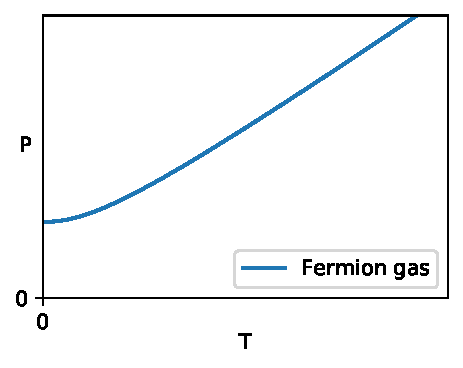
\includegraphics[width=0.725\textwidth]{figs/week09_pressure.pdf}\end{center}
% ------------------------------------------------------------------



% ------------------------------------------------------------------
\subsection{Type-Ia supernovas}
The positive pressure that remains for a fermion gas even at zero temperature, \eq{eq:degen_pressure}, is known as the \textit{degeneracy pressure}.
(This use of the word `degenerate' is completely unrelated to its other use describing multiple energy levels with the same value of the energy.)
The degeneracy pressure plays a key role in a famous cosmic phenomenon---a certain class of supernova explosions of stars.

As a opening remark to this topic, note that the temperature doesn't need to be exactly zero in order for the degeneracy pressure to be significant.
The temperature just needs to be small compared to the Fermi energy, $T \ll E_F$.
From \eq{eq:Fermi_energy} we can see that $E_F \propto \rho_{\text{f}}^{2 / 3}$ increases for larger densities $\rho_{\text{f}} = \vev{N}_{\text{f}} / V$.
Not surprisingly, the densities of stars can be very large indeed, due to the enormous amount of matter that is being squeezed together by gravitational attraction.
Everyday matter has densities around $10^{28}$--$10^{29}$ atoms per cubic metre (roughly corresponding to Avogadro's number per cubic centimetre), which results in Fermi energies $E_F \sim 10^4$~K. % 2--10 eV with eV~10^4 K being the Boltzmann constant
Fermi energies for particularly dense stars known as \textit{white dwarfs} are a hundred thousand times larger, $E_F \sim 10^9$~K, corresponding to densities of roughly one tonne per cubic centimetre.
This is around a million times more dense than our sun---while white dwarf stars have a mass similar to our sun's $M_{\odot}$, their radius is a hundred times smaller, comparable to the radius of the earth.

White dwarf stars are so dense because they have exhausted the hydrogen and helium `fuel' for the nuclear fusion that generates heat and light---and therefore radiation pressure---in stars such as our sun.
For actively `burning' stars, this radiation pressure counteracts the gravitational attraction of the star's enormous mass.
Without nuclear fusion, white dwarfs end up gravitationally compressed into much denser and more compact objects.
The degeneracy pressure, \eq{eq:degen_pressure}, coming from the (fermionic) electrons in the white dwarf is what stabilizes these stars and prevents them from collapsing further into even denser objects such as black holes.

It is remarkable that even under these extreme conditions the electrons in white dwarf stars are well described by the non-interacting ideal fermion gas we have analyzed above.
In particular, it is crucial that white dwarfs' Fermi energies are so large, $E_F \sim 10^9$~K.
Even though white dwarfs have burned all their nuclear fuel, their interiors remain quite hot by everyday standards, roughly ten million kelvin ($T \sim 10^7$~K). % 0.3 MeV ~ 10^5 eV with eV~10^4 K being the Boltzmann constant
It is only due to their large densities and Fermi energies that $T \ll E_F$ and white dwarfs can be treated as zero-temperature objects to a good approximation.

So far we've seen no sign of supernovas.
In isolation, white dwarfs will happily cool for trillions of years, supported by their degeneracy pressure, until they reach thermal equilibrium with the $T_{\text{CMB}} \approx 2.725$~K cosmic microwave background radiation we considered last week. % TODO: CMB temperature will also keep decreasing as universe continues expanding...
Things become more interesting for a white dwarf that forms a binary system with a companion star.
If this companion star that is still burning hydrogen or helium through nuclear fusion, it will emit matter that is then captured by the white dwarf, slowly increasing the white dwarf's mass.
Such a binary system is pictured below, in an artist's illustration provided by the \href{https://www.esa.int/ESA_Multimedia/Images/2014/09/Artist_s_impression_of_Type_Ia_supernova}{European Space Agency}.

\begin{center}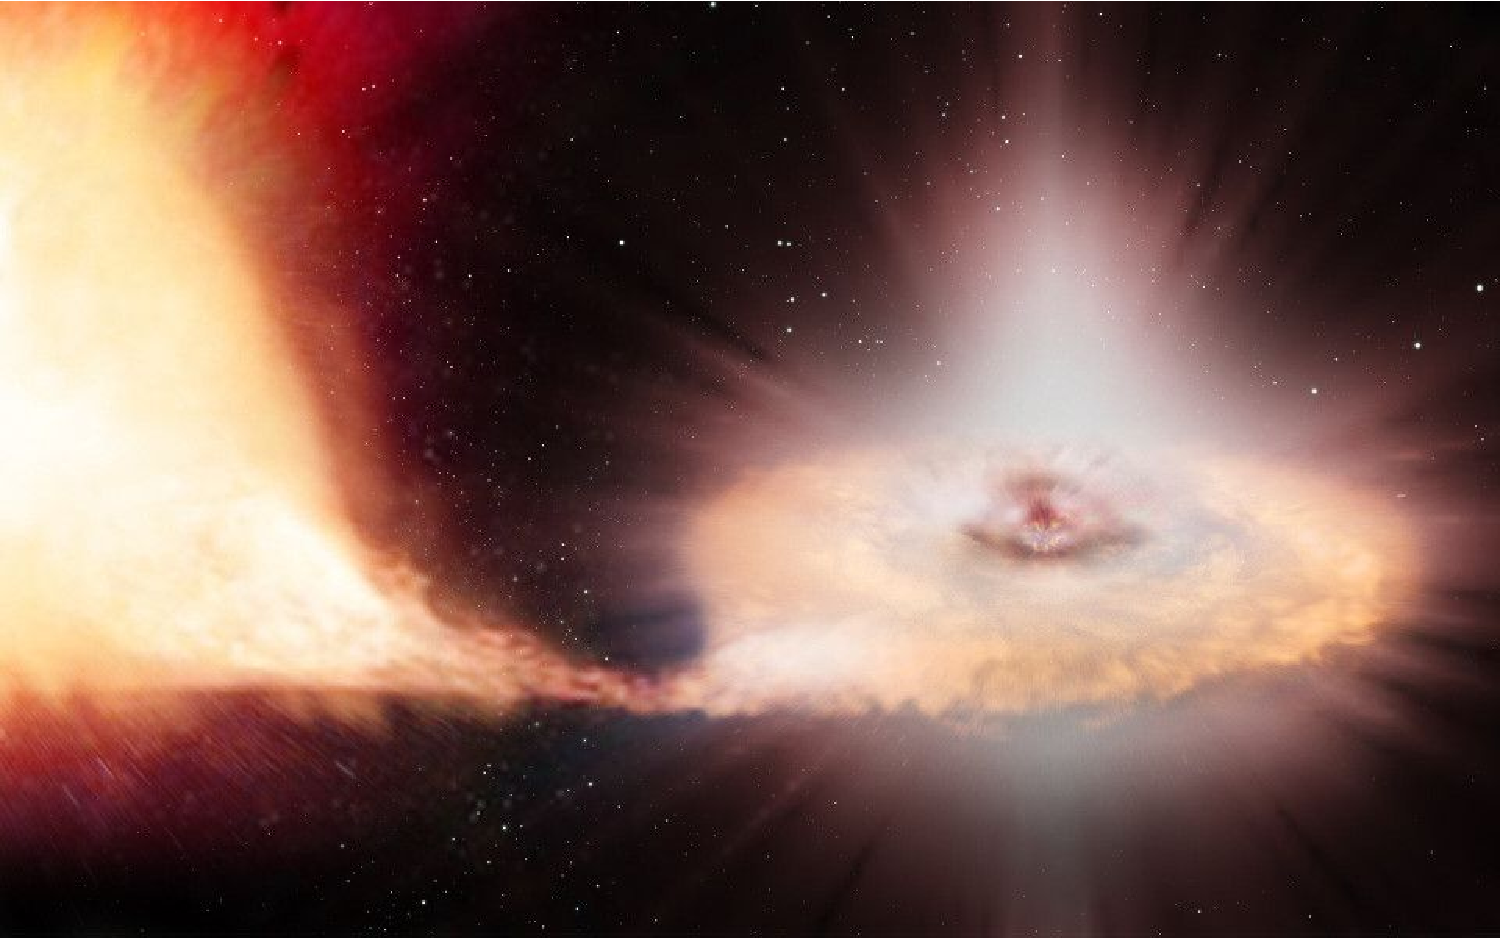
\includegraphics[width=0.8\textwidth]{figs/week09_nova.pdf}\end{center}

As the white dwarf accumulates the matter emitted by its companion, its mass and its density will steadily increase.
As the mass of the white dwarf approaches a value about 40\% larger than the mass of our sun (known as the Chandrasekhar limit, named after \href{https://en.wikipedia.org/wiki/Subrahmanyan_Chandrasekhar}{Subrahmanyan Chandrasekhar}), its density becomes large enough for new types of nuclear fusion reactions to occur.
Instead of hydrogen or helium, which the white dwarf has already burned, these new fusion reactions involve carbon and oxygen, which the white dwarf has in plenty.
In the space of just a few seconds, these fusion reactions run away, increase the temperature of the white dwarf to billions of kelvin, and blast it apart in a supernova explosion about five billion times brighter than the sun.

For obscure historical reasons, these particular stellar explosions are known as \textit{type-Ia} (``one-A'') \textit{supernovas}.
They rely on the degeneracy pressure (\eq{eq:degen_pressure}) of a low-temperature gas of non-interacting fermions, which allows a specific amount of mass to build up before the explosion is triggered.
The specificity of the process results in a great deal of regularity among type-Ia supernovas, which is very useful to astronomers.
In particular, these type Ia supernovas play a key role in demonstrating that the expansion of the universe is accelerating (a phenomenon popularly called `dark energy'), which was awarded the 2011 Nobel Prize in Physics.
% ------------------------------------------------------------------



% ------------------------------------------------------------------
\subsection{Relativistic ideal fermion gas}
While our main focus this week is on non-relativistic gases with $E \propto p^2$, gases of relativistic fermions also appear in nature.
In fact, by changing units we can see that the white dwarf Fermi energy discussed above, $E_F \sim 10^9~\text{K} \sim 0.3$~MeV is comparable to the $0.511$~MeV rest-energy of electrons, suggesting that relativistic effects may be non-negligible in white dwarfs.
Such relativistic effects were indeed taken into account by Chandrasekhar and others investigating these compact stars in the twentieth century.
While the full calculations required to analyze massive relativistic particles are beyond the scope of this module, we can benefit from last week's consideration of gases of massless photons to briefly consider similar gases of massless fermions.
\textit{Neutrinos} (denoted `$\nu$') are physical examples of particles whose masses are so small that they can be very well approximated as massless fermions.\footnote{Neutrinos' masses are so small that it was extremely difficult to determine that they are not exactly massless.  The 2015 Nobel Prize in Physics was awarded for this discovery.}

In the same way as photons, such massless fermions travel at the speed of light, $c$, and have energies $E = cp$ that depend on their angular frequencies,
\begin{equation}
  E_{\nu} = \hbar \om.
\end{equation}
In a volume $V = L^3$, these energies are quantized as usual,
\begin{equation*}
  \om = \frac{2\pi c}{\la} = c \frac{\pi}{L} k,
\end{equation*}
where $k^2 = k_x^2 + k_y^2 + k_z^2$ and $k_{x, y, z} > 0$ are positive integers.
Just as for the massive fermions considered in \secref{sec:fermi_nonrel}, for each distinct set of integers $\vec k = (k_x, k_y, k_z)$, typical massless fermions such as neutrinos have two degenerate energy levels with the same energy.

The detailed analysis of a gas of massless fermions is nearly the same as the work we did last week for photon gases.
In particular, massless fermions are also well described by a vanishing chemical potential, $\mu \approx 0$.
Again approximating sums over discrete integer $k_{x, y, z}$ by integrals over continuous real $\khat_{x, y, z}$, and changing variables to integrate over the angular frequency, we end up with the grand-canonical potential
\begin{align}
  \Phi_{\nu} = -\frac{VT}{c^3 \pi^2} \int_0^{\infty} d\om \; \om^2 \log\left[1 + e^{-\be \hbar \om}\right]. \label{eq:neutrino_grand}
\end{align}
The only change in $\Phi_{\nu}$ compared to \eq{eq:photon_grand} for photons are a couple of negative signs, precisely as we would expect from comparing the Bose--Einstein and Fermi--Dirac grand-canonical potentials in \secref{sec:quantum_classical}.

Carrying out the derivatives to obtain the average particle number density and the average internal energy density produces
\begin{align}
  \frac{\vev{E}_{\nu}}{V} & = \frac{1}{c^3 \pi^2} \int_0^{\infty} \frac{\hbar \om^3}{e^{\be \hbar \om} + 1} d\om &
  \frac{\vev{N}_{\nu}}{V} & = \frac{1}{c^3 \pi^2} \int_0^{\infty} \frac{\om^2}{e^{\be \hbar \om} + 1} d\om,
\end{align}
now differing only by negative signs in their denominators compared to the photon gas results we obtained last week.
The condition of constant entropy is still $V T^3 = \mbox{constant}$, and the resulting pressure leads to an equation of state in the usual form,
\begin{equation*}
  P_{\nu} V \propto \vev{N}_{\nu} T,
\end{equation*}
with the constant of proportionality another $\cO(1)$ number involving the Riemann zeta function.
% ------------------------------------------------------------------


\newpage
% ------------------------------------------------------------------
\renewcommand{\thisweek}{MATH327 Week 10}
\renewcommand{\moddate}{Last modified 4 May 2021}
\setcounter{section}{10}
\setcounter{subsection}{0}
\phantomsection
\addcontentsline{toc}{section}{Week 10: Interacting systems}
\section*{Week 10: Interacting systems}
\subsection{From non-interacting spins to the Ising model}
So far in this module we have considered `ideal' systems whose constituent objects do not interact with each other.
While we have seen that excellent mathematical models for real physical systems (such as stars and the cosmic microwave background) can be obtained despite this approximation of non-interacting particles, there are important statistical physics phenomena that cannot be captured by this approach.

An important class of examples, which we will investigate this week, are \textbf{phase transitions}, where interactions allow the same particles to produce extremely different large-scale behaviours, depending on control parameters such as the temperature or pressure.
An everyday example is the transition of H$_2$O molecules from liquid water to solid ice as the temperature decreases.
As the temperature of the universe itself decreased during the first few micro-seconds following the big bang, elementary particles transitioned from a so-called quark--gluon plasma to the protons and neutrons we are made out of today.
An intermediate example illustrated in the figure below (\href{https://doi.org/10.1063/PT.3.4384}{source}) involves two layers of graphene at a low temperature $T \approx 1.7$~K.
If these two layers are rotated with respect to each other by a small ``magic angle'' $\theta \approx 1.1^{\circ}$, the system transitions from being an electrical insulator to being a superconductor.

\begin{center}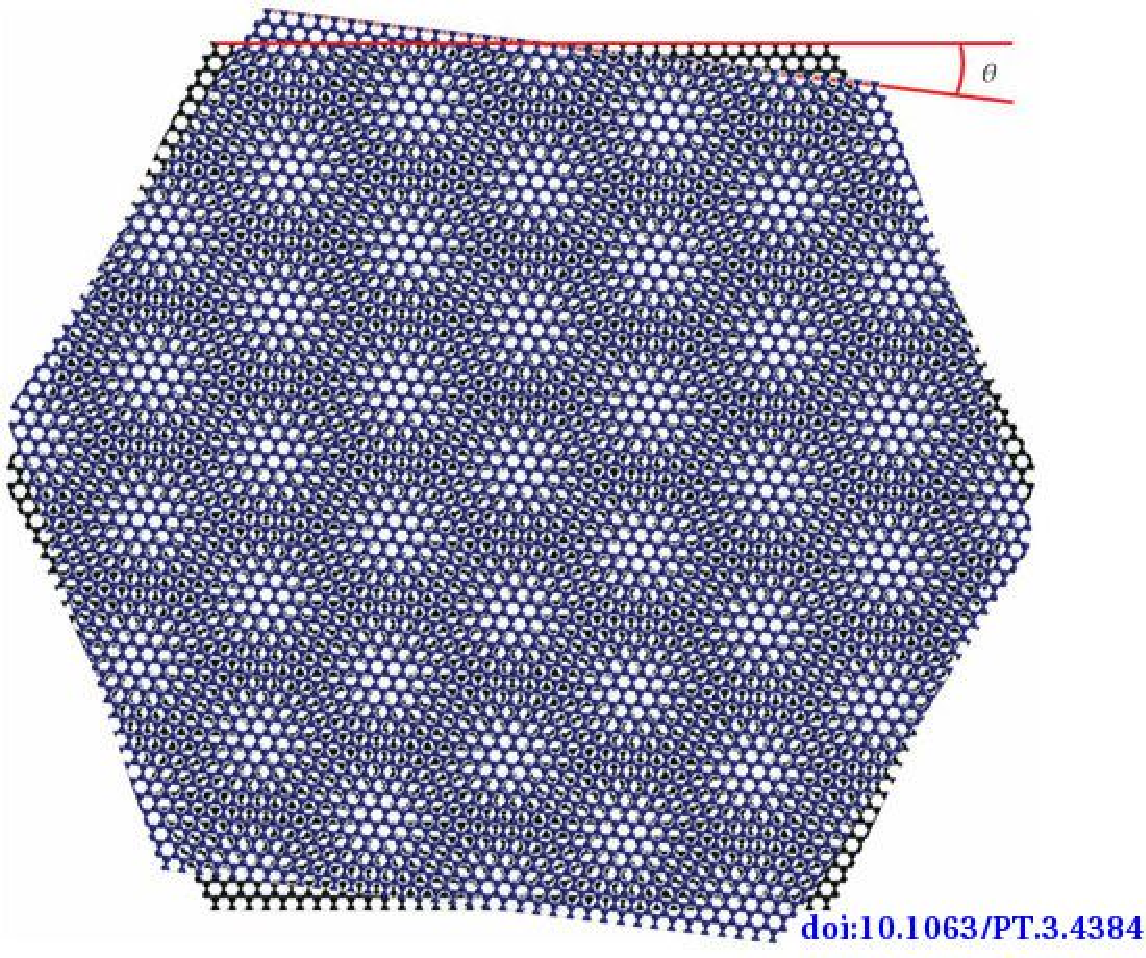
\includegraphics[width=0.5\textwidth]{figs/week10_graphene.pdf}\end{center}

We will introduce interactions and explore their effects using simple spin systems of the sort we previously analyzed in some depth during weeks $2$ and $3$.
In the non-interacting case we previously considered, the internal energy of the system (\eq{eq:spin_energy}) is
\begin{equation*}
  E = H \sum_{n = 1}^N s_n \qquad \mbox{(non-interacting)},
\end{equation*}
where $H > 0$ is the constant strength of an external magnetic field and the orientation of the $n$th spin, $s_n$, takes one of only two possible values: $s_n = 1$ if the spin is aligned anti-parallel to the field and $s_n = -1$ if the spin is aligned parallel to the field.
The ground state of the system features all $N$ spins aligned parallel to the magnetic field, with minimal energy $E_0 = -NH$.
This week we will only consider systems of distinguishable spins, which can be labeled by their fixed position in a $d$-dimensional simple cubic \textbf{lattice} like that shown below for $d = 2$ dimensions.
The $d = 1$ case of a one-dimensional lattice is precisely the system of spins arranged in a line that we analyzed in \secref{sec:spin_chain}.

\begin{center}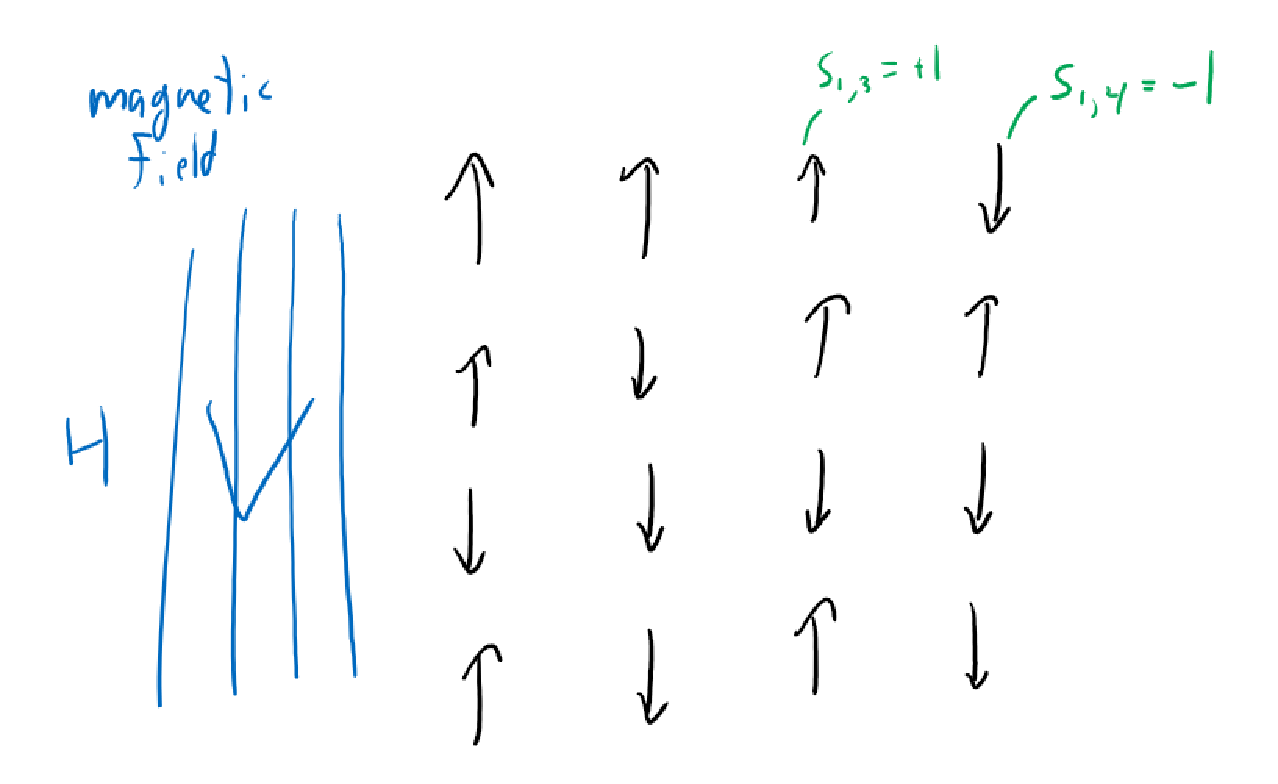
\includegraphics[width=0.8\textwidth]{figs/week10_spins.pdf}\end{center}

We can see that the total internal energy of the non-interacting system can easily be written as a sum over energies for each individual spin,
\begin{align*}
  E_n & = H s_n &
  E & = \sum_{n = 1}^N E_n \qquad \mbox{(non-interacting)}.
\end{align*}
This is a generic feature of non-interacting systems, and an aspect of the \textbf{factorization} that enormously simplifies calculations by causing the $N$-particle partition function (\eq{eq:spin_part_func}) to take the form of a product of $N$ identical terms, $Z = \left[2\cosh\left(\be H\right)\right]^N = Z_1^N$.
However, a stronger condition needs to be satisfied in order for such factorization to be guaranteed, which rigorously defines what it means for a system to be non-interacting.

\begin{shaded}
  Let $\De E_i$ be the change in the system's internal energy caused by changing its $i$th degree of freedom.
  Then the system is defined to be \textbf{non-interacting} if and only if $\De E_i$ is independent of all other degrees of freedom $k \ne i$.
\end{shaded}

For our system of $N$ distinguishable spins, the only possible change we can make to a degree of freedom is to negate it, $s_i \to -s_i$, which corresponds to flipping its alignment relative to the external magnetic field.
This spin flip causes the total energy to change,
\begin{equation*}
  E = H \sum_{n = 1}^N s_n = H\left(s_i + \sum_{k \ne i} s_k\right) \quad \lra \quad H\left(-s_i + \sum_{k \ne i} s_k\right),
\end{equation*}
corresponding to $\De E_i = -2H s_i$, which is indeed independent of all spins $s_k$ with $k \ne i$.
This simple check confirms that our definition works for the non-interacting spin system under consideration.

Now let's convert this setup into a system of interacting spins by adding the simplest possible two-spin contribution to its energy:
\begin{equation}
  \label{eq:Ising_energy}
  E = -\sum_{(ij)} s_i s_j + H \sum_{n = 1}^N s_n.
\end{equation}
The first sum runs over all pairs of nearest-neighbour spins in the lattice, denoted $(ij)$.
What is the change in energy $\De E_i$ from \eq{eq:Ising_energy} upon negating $s_i \to -s_i$?
Does this indicate an interacting or non-interacting system?
\begin{mdframed}
  \ \\[100 pt]
\end{mdframed}
The pictures below illustrate nearest-neighbour pairs for simple cubic lattices in $d = 2$ and $3$ dimensions, while also introducing some additional lattice terminology.

\begin{center}
  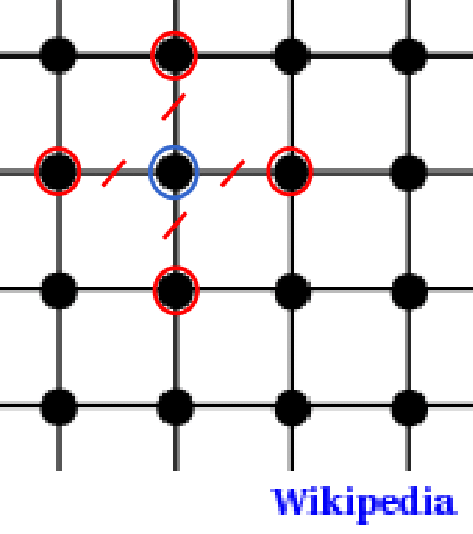
\includegraphics[height=0.4\textwidth]{figs/week10_lattice_2d.pdf}\hfill
  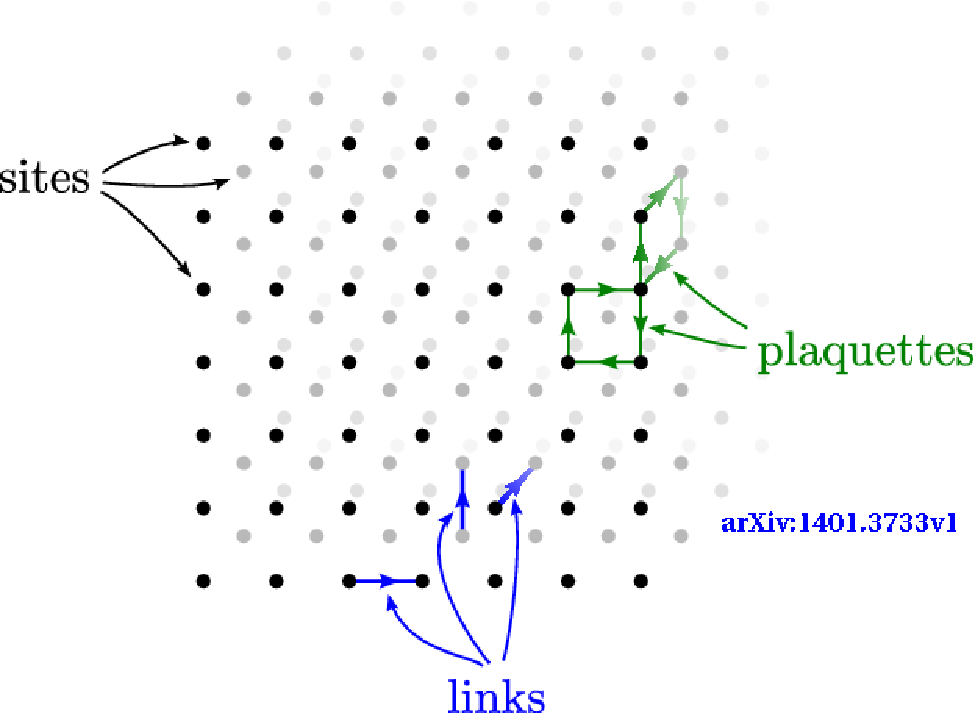
\includegraphics[height=0.4\textwidth]{figs/week10_lattice_3d.pdf}
\end{center}

Instead of drawing up- and down-pointing arrows, these pictures identify the spins with \textit{sites} in the lattice represented as points (or larger filled circles).
In simple cubic lattices, all sites are positioned in a regular grid, separated by a constant distance along each basis vector.
In between nearest-neighbour sites, we can draw \textit{links} as solid lines.
The picture of a two-dimensional lattice on the left highlights the four links (with red hatch marks) that correspond to the four nearest neighbours (circled in red) of a particular site (circled in blue).
While we can only have physical lattices with $d = 1$, $2$ or $3$ in nature, the mathematical construction works just as well for any integer $d \geq 1$.
For $d \geq 2$, an elementary unit of surface area is called a \textit{plaquettes}, while for $d \geq 3$ the elementary unit of volume is called a \textit{cube}.

Computing the energy in \eq{eq:Ising_energy} requires determining all of the nearest-neighbour pairs to be summed in the first term, which is equivalent to all of the links in the lattice, $\ell = (ij)$.
The only potential complication to this task is the need to consider what happens at the edges of the (finite) lattice.
We can avoid this complication by imposing \textbf{periodic boundary conditions}, which add an extra link between each site on the left edge of the lattice and a corresponding site on the right edge (and similarly in all other dimensions).
This is illustrated below for the simple one-dimensional lattice, which has been drawn as a circle to emphasize that all $N$ sites remain separated by a constant distance.
In higher dimensions, periodic boundary conditions produce flat (zero-curvature) $d$-dimensional tori that preserve the simple cubic lattice structure.

\begin{center}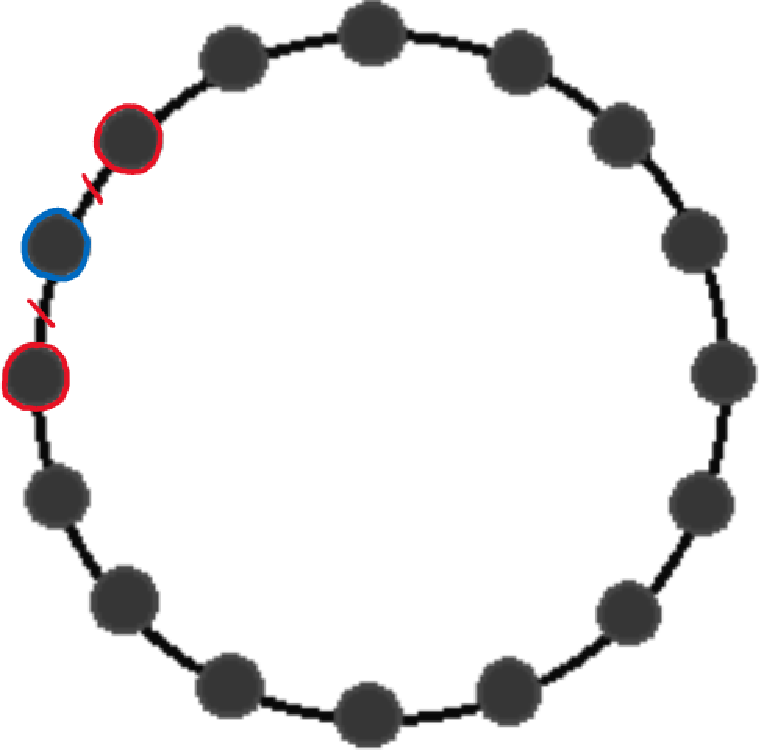
\includegraphics[width=0.45\textwidth]{figs/week10_lattice_1d.pdf}\end{center}

With periodic boundary conditions, we can easily see that the $N$-site one-dimensional lattice drawn above has $N$ links.
Each site has two links connecting it to its two nearest neighbours, and each of those links is shared between two sites, so that $\#\ell = 2N / 2 = N$.
Looking back to the two-dimensional lattice drawn farther above, the four links per site produce $\#\ell = 4N / 2 = 2N$.
How many terms are there in the sum $\sum_{(ij)}$ in \eq{eq:Ising_energy} for $N$-site lattices with periodic boundary conditions in $d$ dimensions?
\begin{mdframed}
  \ \\[50 pt]
\end{mdframed}

The energy in \eq{eq:Ising_energy}, with nearest-neighbour spins specified by the underlying simple cubic lattice structure, defines a famous system known as the $d$-dimensional \textbf{Ising model}.
Since the 1960s, the Ising model has been the basis of thousands of scientific studies analyzing everything from ferromagnetism to neural networks to urban segregation.\footnote{For a brief summary, see Charlie Wood, ``\href{https://www.quantamagazine.org/the-cartoon-picture-of-magnets-that-has-transformed-science-20200624/}{The Cartoon Picture of Magnets That Has Transformed Science}'', \textit{Quanta Magazine}, 24 July 2020.}
The model was proposed in 1920 by \href{https://en.wikipedia.org/wiki/Wilhelm_Lenz}{Wilhelm Lenz}, whose PhD student \href{https://en.wikipedia.org/wiki/Ernst_Ising}{Ernst Ising} solved the one-dimensional system as a research project in 1924.
Exactly solving the two-dimensional case (with $H = 0$) took another twenty years, culminating in renowned work by \href{https://en.wikipedia.org/wiki/Lars_Onsager}{Lars Onsager} in 1944.
The three-dimensional Ising model remains an open mathematical question, with no known exact solution.

In this context, `solving' the Ising model means deriving a closed-form expression for its canonical partition function,
\begin{equation*}
  Z(\be, N, H) = \sum_{\left\{s_n\right\}} \exp\left[-\be E(s_n)\right] = \sum_{\left\{s_n\right\}} \exp\left[\be\sum_{(ij)} s_i s_j - \be H \sum_n s_n\right].
\end{equation*}
As in \secref{sec:spin_info}, the partition function sums over all possible spin configurations $\left\{s_n\right\}$, which amounts to a sum of $2^N$ exponential factors for $N$ spins, with $\cO(N)$ terms within each exponential.
Now that the system is interacting, the partition function can no longer be factorized into $N$ identical two-term factors, making it extremely difficult to evaluate.
This is why there is no known exact solution to the three-dimensional Ising model, and it also makes `brute-force' numerical computations impractical.
Even for a system of $N = 1023$ spins (tiny compared to Avogadro's number $\sim 10^{23}$) there would be roughly $2^{1023} \sim 10^{310}$ terms in the partition function, far beyond the capabilities of existing or foreseeable supercomputers.
% ------------------------------------------------------------------



% ------------------------------------------------------------------
\subsection{Ising model phases and phase transition}
Similarly to how we analyzed non-interacting spin systems in \secref{sec:spin_info}, we can simplify the Ising model by considering its behaviour in the limits of high and low temperatures.
For another simplification, we will set $H = 0$ in this section, and consider
\begin{align}
  \label{eq:Ising_zero_field}
  E & = -\sum_{(ij)} s_i s_j &
  Z(\be, N) & = \sum_{\left\{s_n\right\}} \exp\left[\be\sum_{(ij)} s_i s_j\right].
\end{align}
We will see that the large-scale behaviour of the Ising model is qualitatively different at high temperatures compared to low temperatures.
In other words, the system exhibits two distinct phases for different temperatures.
This is a necessary but not sufficient condition for there to be a true phase transition---a priori, it is possible for there to be a gradual \textit{crossover} between these two phases, as opposed to a rapid transition.
We will use the Ising model to more rigorously define what exactly constitutes a phase transition, and how this can be distinguished from a crossover.

\newpage % WARNING: FORMATTING BY HAND
The Ising model partition function becomes extremely simple in the \textbf{high-temperature} limit $\be \to 0$.
What is its asymptotic limit?
\begin{mdframed}
  $\displaystyle Z(\be = 0, N) = $ \\[50 pt]
\end{mdframed}
You should find a result identical to that for a micro-canonical system with energy $E = 0$, which is clearly non-interacting since $\De E_i = 0$.
Every spin configuration is a different micro-state of the system, all with the same probability $p_i = 1 / 2^N$, as in \eq{eq:micro_equil}.

Effectively, we are considering temperatures so high that the energy from \eq{eq:Ising_zero_field} is negligible for any spin configuration.
Although the energy no longer distinguishes between different micro-states, we can define a quantity that continues to be sensitive to the details of the spin configuration.
This is the \textbf{magnetization} $M = n_+ - n_-$, where we redefine $n_{\pm}$ to be the number of spins with value $\pm 1$, so that $N = n_+ + n_-$.\footnote{In week $2$ we defined $n_{\pm}$ based on spins' alignment with or against the external magnetic field, which no longer applies now that we have set $H = 0$.}
It is convenient to normalize the total magnetization $M$ by the number of spins,
\begin{equation}
  \label{eq:Ising_magnet}
  |m| \equiv \frac{|M|}{N} = \frac{|n_+ - n_-|}{n_+ + n_-}
\end{equation}
so that $0 \leq |m| \leq 1$ for any value of $N$.

Our task is now to determine the expectation value of the magnetization at high temperatures.
Above we found that all spin configurations are equally probable in this regime, so $\vev{|m|}$ will be determined by how likely it is for these micro-states to have a particular magnetization.
For example, there are only two micro-states with $|m| = 1$, corresponding to $(n_+, n_-) = (N, 0)$ and $(0, N)$.
In general, just as we saw in \eq{eq:spin_states}, there are
\begin{equation*}
  \binom{N}{n_+} = \binom{N}{n_-} = \frac{N!}{n_+! \; n_-!}
\end{equation*}
equally probable micro-states with a given $n_+ = N - n_-$.
For large $N \gg 1$ this binomial coefficient is factorially peaked around
\begin{equation*}
  n_+ = n_- = \frac{1}{2} N \qquad \lra \qquad |m| = 0,
\end{equation*}
which defines a \textbf{disordered phase} with similar numbers of up- and down-pointing spins producing a small magnetization.
In the so-called \textit{thermodynamic limit} $N \to \infty$, the expectation value of the magnetization in the disordered phase vanishes exactly, $\vev{|m|} \to 0$.

We now need to determine $\vev{|m|}$ in the \textbf{low-temperature} limit $\be \to \infty$.
In this regime, as we saw in \secref{sec:spin_chain}, the Boltzmann factor $\exp\left[\be\sum_{(ij)} s_i s_j\right]$ makes it exponentially more likely for the system to adopt micro-states with lower energies.
In particular, we can expect the ground state to dominate the expectation value of the magnetization, $\vev{|m|}$, up to exponentially suppressed corrections from higher-energy excited states.
With $H = 0$, the Ising model has two degenerate ground states corresponding to the two ways all the spins can be aligned with each other: $(n_+, n_-) = (N, 0)$ and $(0, N)$.
What is the ground-state energy of the $N$-site Ising model in $d$ dimensions?
\begin{mdframed}
  $\displaystyle E_0 = -\sum_{(ij)} s_i s_j = $ \\[50 pt]
\end{mdframed}

As mentioned above, both of these degenerate ground states have the maximal magnetization $|m| = 1$.
Let's check what effect the first excited state would have on the overall magnetization of the system.
The first excited state involves negating (or `flipping') a single spin, corresponding to $(n_+, n_-) = (N - 1, 1)$ and $(1, N - 1)$.
Because any one of the $N$ spins in the lattice could be flipped, the degeneracy of the first excited state grows with $N$:
\begin{equation*}
  \binom{N}{1} + \binom{N}{N - 1} = 2N.
\end{equation*}
At the same time, as $N$ increases the magnetization of each of these micro-states gets closer to that of the ground state,
\begin{equation*}
  |m| = \frac{N - 1}{N} = 1 - \frac{1}{N}.
\end{equation*}
The key factor is the probability for the system to be in one of these micro-states, which depends on the energy of the first excited state, $E_1$.
What is the first-excited-state energy of the $N$-site Ising model in $d$ dimensions?
\begin{mdframed}
  $\displaystyle E_1 = $ \\[100 pt]
\end{mdframed}

Let's put things together by computing the relative probability for the $d$-dimensional Ising model to be in its ground state with $|m| = 1$ compared to its first excited state with $|m| = 1 - \frac{1}{N}$, accounting for the different number of micro-states in each case:
\begin{equation*}
  \frac{p(E_0)}{p(E_1)} = \frac{2\cdot \exp\left[\be d\cdot N\right]}{2N\cdot \exp\left[\be \left(d\cdot N - 4d\right)\right]} = \frac{\exp\left[4\be d\right]}{N}.
\end{equation*}
For any fixed $N$, a sufficiently low temperature will cause the ground state to dominate.
This defines an \textbf{ordered phase} in which essentially all spins are aligned in the same direction, producing a large expectation value for the magnetization, $\vev{|m|} = 1$.

We have seen that the magnetization $\vev{|m|}$ distinguishes between the high- and low-temperature behaviour of the $d$-dimensional Ising model.
In the high-temperature disordered phase, the magnetization is small and $\vev{|m|} \to 0$ in the thermodynamic limit $N \to \infty$.
In the low-temperature ordered phase, the magnetization is large and $\vev{|m|} \to 1$ as $T \to 0$.
This is typical behaviour for interacting statistical systems, where the quantity distinguishing between these two phases (here the magnetization) is known as the \textbf{order parameter}.
The behaviour of the order parameter is what distinguishes gradual crossovers from rapid phase transitions.

\begin{shaded}
  A phase transition is characterized by a discontinuity in the order parameter or its derivative(s), in the $N \to \infty$ thermodynamic limit.
  The value(s) of the control parameter(s) at which the discontinuity occurs define the \textit{critical point} corresponding to the transition.
\end{shaded}

For the zero-field ($H = 0$) Ising model, the control parameter is the temperature $T$, and any phase transition would occur at a \textbf{critical temperature} $T_C$.
The sketches below illustrate the most common types of phase transitions.
When the order parameter (OP) itself is discontinuous (shown by a dashed line), the transition is said to be a \textit{first-order} phase transition.
When the order parameter is continuous at $T_C$ but its first derivative is discontinuous, the transition is said to be a \textit{second-order} phase transition.
This naming scheme generalizes to higher-order phase transitions, the most remarkable of which is the infinite-order BKT phase transition (named after \href{https://en.wikipedia.org/wiki/Vadim_Berezinskii}{Vadim Berezinskii}, \href{https://en.wikipedia.org/wiki/J._Michael_Kosterlitz}{J.\ Michael Kosterlitz} and \href{https://en.wikipedia.org/wiki/David_J._Thouless}{David Thouless}), which was awarded the 2016 Nobel Prize in Physics.

\begin{center}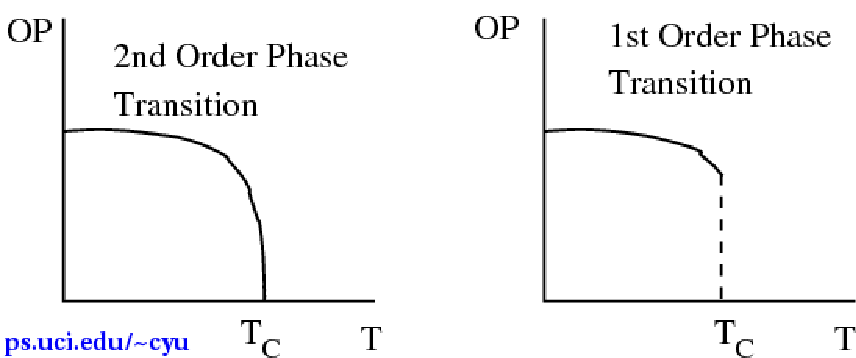
\includegraphics[width=0.8\textwidth]{figs/week10_transitions.pdf}\end{center}

Because true discontinuities are only possible with an infinite number of degrees of freedom, it is really the way in which the system approaches the $N \to \infty$ thermodynamic limit that distinguishes crossovers from true phase transitions.
We will conclude this week's consideration of interacting systems by developing a useful approximation for the Ising model, which will turn out to be more reliable as the dimensionality $d$ increases.
% ------------------------------------------------------------------



% ------------------------------------------------------------------
\subsection{The mean-field approximation}
Looking back to \eq{eq:Ising_magnet}, we can identify the magnetization (with no absolute value) as the average spin,
\begin{equation*}
  m = \frac{M}{N} = \frac{1}{N}\left(n_+ - n_-\right) = \frac{1}{N} \sum_{n = 1}^N s_n.
\end{equation*}
The `mean' in the mean-field approximation refers to the expectation value of the average spin,
\begin{equation*}
  \vev{m} = \frac{1}{Z} \sum_{\left\{s_n\right\}} m \; e^{-\be E(s_n)} = \frac{1}{N} \sum_{n = 1}^N \vev{s_n},
\end{equation*}
which is independent of the spin configuration $\left\{s_n\right\}$ and is simply a function of the inverse temperature \be and magnetic field strength $H$.\footnote{To be consistent with the redefinition of $n_{\pm}$ above \eq{eq:Ising_magnet}, we reverse our sign convention for the magnetic field, $H \to -H$.}
By adding and subtracting factors of $\vev{m}$, we can exactly rewrite each nearest-neighbour term in the Ising model energy, \eq{eq:Ising_energy}, as
\begin{align}
  s_i s_j & = \left[\left(s_i - \vev{m}\right) + \vev{m}\right] \times \left[\left(s_j - \vev{m}\right) + \vev{m}\right] \cr
          & = \left(s_i - \vev{m}\right) \left(s_j - \vev{m}\right) + \left(s_i + s_j\right)\vev{m} - \vev{m}^2. \label{eq:MF_start}
\end{align}

The factors of $\left(s_i - \vev{m}\right)$ correspond to the spins' fluctuations around their mean value $\vev{m}$.
By conjecturing that these fluctuations are small \textit{on average}, we can approximate the Ising model energy by neglecting the first term in \eq{eq:MF_start} when summing over all links:
\begin{equation*}
  E = -\sum_{(ij)} s_i s_j - H \sum_{n = 1}^N s_n \quad \lra \quad \EMF = -\sum_{(ij)} \left[\left(s_i + s_j\right)\vev{m} - \vev{m}^2\right] - H \sum_{n = 1}^N s_n.
\end{equation*}
The sum over the links $\ell = (ij)$ in $d$ dimensions simply counts $d\cdot N$ factors of the constant $\vev{m}^2$.
Similarly, since the first term includes both spins $\left(s_i + s_j\right)$ on each end of the link, every individual spin appears $2d$ times in the sum over links, which we can combine with the sum over sites:
\begin{equation}
  \label{eq:MF_energy}
  \EMF = d\cdot N \vev{m}^2 - \left(2d\vev{m} + H\right) \sum_{n = 1}^N s_n \equiv d\cdot N \vev{m}^2 - H_{\text{eff}} \sum_{n = 1}^N s_n,
\end{equation}
\newpage % WARNING: FORMATTING BY HAND
\noindent defining an effective magnetic field $H_{\text{eff}}$ that depends on the mean spin.
What is the change in energy $\De E_i$ from \eq{eq:MF_energy} upon negating $s_i \to -s_i$?
Does this indicate an interacting or non-interacting system?
\begin{mdframed}
  \ \\[100 pt]
\end{mdframed}

The mean-field approximation producing \eq{eq:MF_energy} makes it very easy to compute the corresponding canonical partition function
\begin{align}
  \ZMF & = \sum_{\left\{s_n\right\}} \exp\left[-\be E(s_n)\right] = \exp\left[-\be d\cdot N \vev{m}^2\right] \sum_{s_1 = \pm 1} \cdots \sum_{s_N = \pm 1} \exp\left[-x \sum_{n = 1}^N s_n\right] \cr
       & = \exp\left[-\be d\cdot N \vev{m}^2\right] \left(2\cosh\left[\be H_{\text{eff}}\right]\right)^N \nonumber \\
       & = \exp\left[-\be d\cdot N \vev{m}^2\right] \left(2\cosh\left[\be \left(2d\vev{m} + H\right)\right]\right)^N,
\end{align}
where we defined $x = -\be H_{\text{eff}}$ to put the sums into exactly the same form as \eq{eq:spin_part_func}.
We see that the mean-field partition function exhibits complicated dependence on $\vev{m}$.
In order to get a handle on this dependence, we need to determine another relation between $\vev{m}$ and $\ZMF$.

We can do this by recalling the connection between the magnetization and the average spin discussed at the start of this section.
Because the total $N$-spin magnetization
\begin{equation*}
  M = n_+ - n_- = \sum_{n = 1}^N s_n,
\end{equation*}
we can write the full Ising model energy as
\begin{equation*}
  E = -\sum_{(ij)} s_i s_j - H \sum_{n = 1}^N s_n = -\sum_{(ij)} s_i s_j - H M,
\end{equation*}
with corresponding canonical partition function
\begin{equation*}
  Z = \sum_{\left\{s_i\right\}} \exp\left[\be \sum_{(ij)} s_i s_j + \be H M\right].
\end{equation*}
\newpage % WARNING: FORMATTING BY HAND
\noindent From our earlier experience with the canonical ensemble, it now comes as no surprise that $\vev{M} = N\vev{m}$ can be related to a derivative of the Helmholtz free energy $F = -T\log Z$.
What is this relation?
\begin{mdframed}
  $\displaystyle \pderiv{}{H} F = $ \\[100 pt]
\end{mdframed}

Returning to the mean-field approximation,
\begin{equation*}
  \log \ZMF = N\log \cosh\left[\be \left(2d\vev{m} + H\right)\right] + \left\{H\mbox{-independent terms}\right\},
\end{equation*}
we can use this relation between $\vev{m}$ and $\ZMF$ to find
\begin{equation*}
  \vev{m} = \frac{1}{N\be} \pderiv{}{H}\log \ZMF = \frac{1}{\be} \frac{1}{\cosh\left[\be \left(2d\vev{m} + H\right)\right]} \pderiv{}{H}\cosh\left[\be \left(2d\vev{m} + H\right)\right].
\end{equation*}
Simplifying, we obtain a \textbf{self-consistency condition} for the magnetization in the mean-field approximation:
\begin{equation}
  \label{eq:consistency}
  \vev{m} = \tanh\left[\be \left(2d\vev{m} + H\right)\right].
\end{equation}
Solving this equation for $\vev{m}$ is equivalent to finding the roots of the equation $\tanh\left[\be (2d\cdot x + H)\right] - x = 0$.

A straightforward way to inspect such solutions is by plotting both
\begin{align*}
  f(\vev{m}) & = \vev{m} &
  g(\vev{m}) & = \tanh\left[\be (2d\vev{m} + H)\right]
\end{align*}
and monitoring the intersections of these two functions.
Fixing $d = 2$ dimensions, the plot below considers the simplest case $\be = \frac{1}{4}$ and $H = 0$ for which $g(\vev{m}) = \tanh\left[\vev{m}\right]$ (the solid line).
There is only a single intersection between this function and $f(\vev{m})$ (the dashed line), at $\vev{m} = 0$.

\begin{center}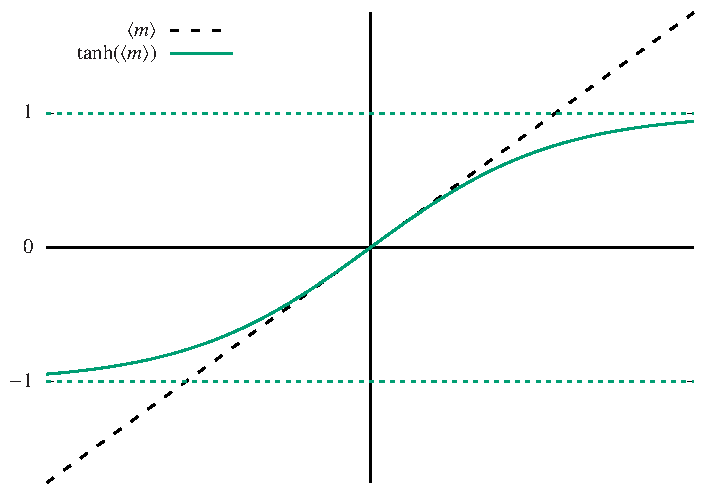
\includegraphics[width=0.7\textwidth]{figs/week10_consistency.pdf}\end{center}

Before interpreting this result, let's check how the intersections depend on \be and $H$.
In the next plot below we keep the same temperature $T = 1 / \be = 4$ while turning the external magnetic field back on.
A positive $H > 0$ simply shifts $g(\vev{m})$ to the left (the green line), while a negative $H < 0$ shifts it to the right (the blue line).
For $H = \pm 2$, there is still only a single intersection, at $\vev{m} \approx \pm 0.88$.
We can see that because $-1 \leq \tanh x \leq 1$, the mean-field self-consistency condition can only ever predict $-1 \leq \vev{m} \leq 1$, in accord with the definition of the magnetization.

\begin{center}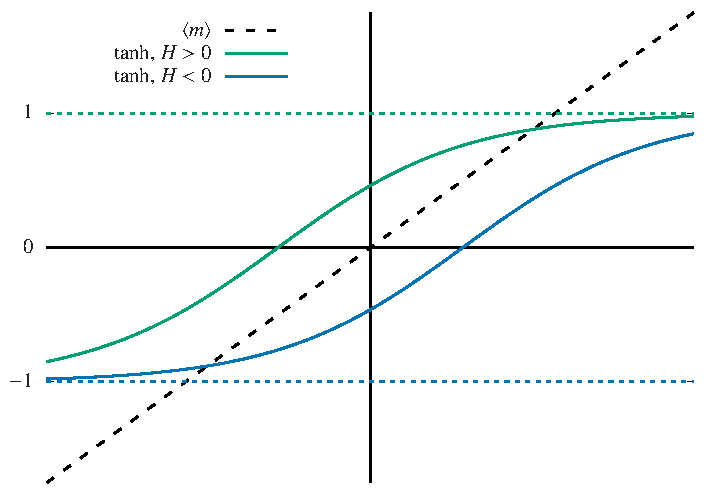
\includegraphics[width=0.7\textwidth]{figs/week10_consistency_H.pdf}\end{center}

Next, if we decrease the temperature, $g(\vev{m})$ becomes steeper, more rapidly interpolating between those limiting values $-1 \leq \tanh x \leq 1$.
The plot below illustrates this for $T = 1 / \be = 2$, so that $\be = \frac{1}{2}$ is doubled.
Already for this temperature and magnetic field $H = \pm 2$, the intersection is $\vev{m} \approx \pm 1$ to a very good approximation.
We can interpret this result as an indication that the system is in an ordered phase where all spins are aligned with the external field.

\begin{center}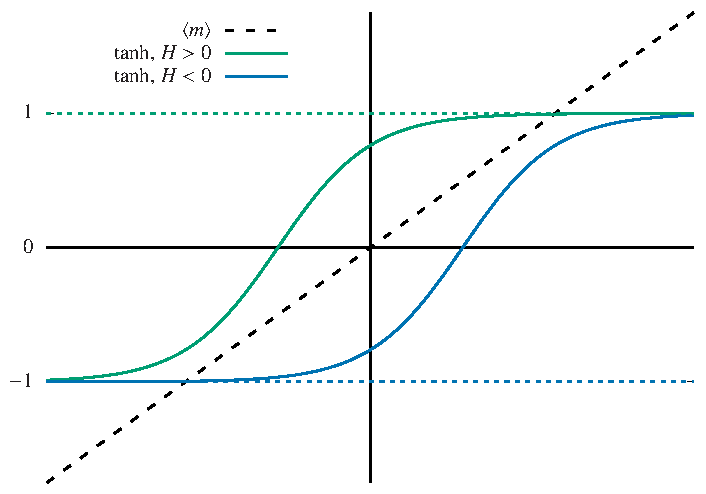
\includegraphics[width=0.7\textwidth]{figs/week10_consistency_H-beta.pdf}\end{center}

To search for a phase transition we need to turn off that external field by setting $H = 0$, and consider how the solutions of the self-consistency condition depend on the temperature.
We do this in the next plot below, considering a low temperature $T = 2$ with $\be = \frac{1}{2}$ (the red line), the same green curve for $T = 4$ shown in the first plot above, and a high temperature $T = 8$ with $\be = \frac{1}{8}$ (the blue line).
While the $\vev{m} = 0$ expected in the disordered phase is always a possible solution, something interesting happens at lower temperatures, where the steeper $\tanh$ function introduces two additional solutions at $\vev{m} = \pm m_0$.
As $T \to 0$, this $m_0 \to 1$, approaching the magnetization of the ordered phase.

\begin{center}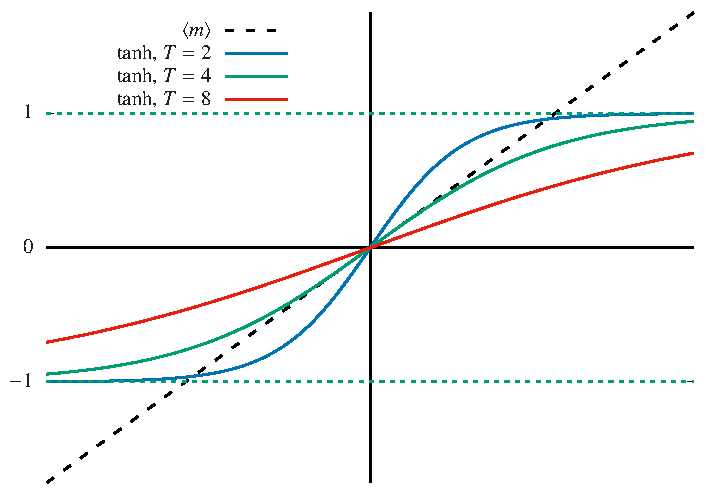
\includegraphics[width=0.7\textwidth]{figs/week10_consistency_beta.pdf}\end{center}

When there are three solutions $\vev{m} = \left\{-m_0, 0, m_0\right\}$ at low temperatures, we can determine that the $\vev{m} = 0$ solution is actually \textit{unstable}.
In this case, the slope of the $\tanh$ at $\vev{m} = 0$ must be greater than $1$.
Any positive value $\vev{m} = \varepsilon > 0$ would therefore produce $\tanh\left[2\be d\vev{m}\right] > \vev{m}$, violating the self-consistency condition in \eq{eq:consistency}.
Since the violation comes from $\vev{m}$ being too small compared to the $\tanh$, $\vev{m}$ would be driven to increase further, until it eventually reached the non-zero solution $\vev{m} = m_0$.
The analogous argument implies any negative value $\vev{m} = -\varepsilon < 0$ would drive $\vev{m}$ away from zero and to the $\vev{m} = -m_0$ solution.

This argument can be visualized by plotting $\tanh\left[2\be d\vev{m}\right] - \vev{m}$ vs.\ $\vev{m}$ as shown in the final plot below.
Whenever this difference is negative, it implies $\vev{m}$ is larger than the self-consistency condition allows, and therefore consistency requires reducing $\vev{m}$, shown by arrows pointing to the left.
Conversely, whenever the difference is positive, $\vev{m}$ would have to increase to recover consistency, shown by the arrows pointing to the right.
For the low temperature $T = 2$, we see that the arrows move the system away from the unstable solution $\vev{m} = 0$ and to the stable solutions $\vev{m} = \pm m_0$.

\begin{center}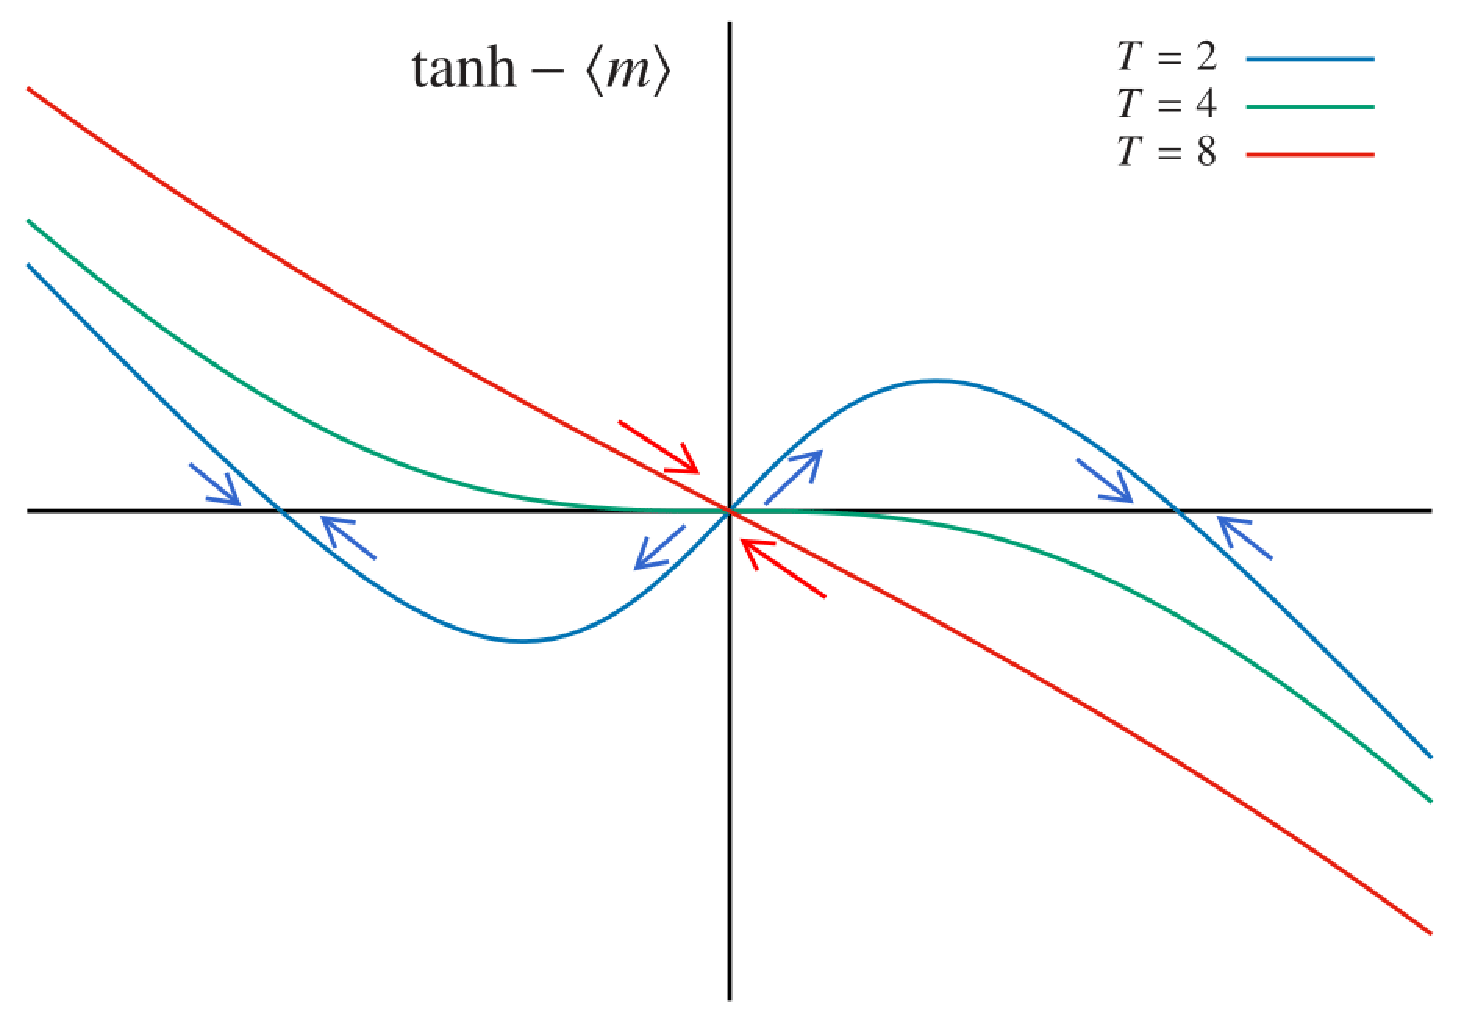
\includegraphics[width=0.7\textwidth]{figs/week10_consistency_flow.pdf}\end{center}

Reassuringly, the mean-field approximation with $H = 0$ therefore reproduces the behaviour we derived in the previous section.
For high temperatures we have $\vev{m} = 0$ consistent with the disordered phase, while for low temperatures we have $|\vev{m}| = m_0 \to 1$ consistent with the ordered phase.
We can also determine the temperature at which the $\vev{m} = \pm m_0$ solutions appear and the $\vev{m} = 0$ solution becomes unstable.
As described above, this occurs whenever the slope of the $\tanh$ function at $\vev{m} = 0$ is greater than $1$.
Using $\tanh(x) = x + \cO\left(x^3\right)$ for $x \approx 0$, what is the slope of this $\tanh$?
\begin{mdframed}
  $\displaystyle \left. \frac{d}{d\vev{m}} \tanh\left[2\be d\vev{m}\right]\right|_{\vev{m} = 0} = $ \\[50 pt]
\end{mdframed}

You should find that the change from the high-temperature disordered phase to the low-temperature ordered phase occurs at $T_c = 2d$ in $d$ dimensions, or equivalently $\be_c = \frac{1}{2d}$.
Despite the subscript, we don't yet know if this $T_c$ is a true critical temperature.
In order to check whether the mean-field approximation of the $H = 0$ Ising model predicts a crossover or a true phase transition, we need to check whether or not the order parameter $\vev{m}$ or its derivatives are discontinuous at $T_c$.
We can do this by considering the self-consistency condition for a temperature $T = 1 / \be$ lower than but close to $T_c = 2d$, which would produce $0 < |\vev{m}| \ll 1$ and allow us to expand
\begin{equation*}
  \vev{m} = \tanh\left[\frac{2d}{T} \vev{m}\right] \approx \frac{T_c}{T} \vev{m} - \frac{1}{3}\left(\frac{T_c}{T} \vev{m}\right)^3.
\end{equation*}
What is the resulting prediction for $\vev{m}$?
\begin{mdframed}
  \ \\[100 pt]
\end{mdframed}

Approximating $\frac{T}{T_c} \approx 1$, your result should resemble
\begin{equation*}
  \vev{m} = \pm \sqrt{3} \left(\frac{T_c - T}{T_c}\right)^{1 / 2} \qquad \mbox{for } \ T \lesssim T_c.
\end{equation*}
From this, we can see that the order parameter $\vev{m}$ is continuous at $T_c$:
\begin{equation}
  \vev{m} \propto \left\{\begin{array}{cl} \left(T_c - T\right)^{1 / 2} & \mbox{for } \ T \lesssim T_c \\[3 pt]
                                           0                            & \mbox{for } \ T \gtrsim T_c\end{array}\right. .
\end{equation}
However, its first derivative
\begin{equation*}
  \frac{d\vev{m}}{dT} \propto \frac{1}{\left(T_c - T\right)^{1 / 2}}
\end{equation*}
diverges as $T \to T_c$ from below, predicting a second-order phase transition with critical temperature $T_c = 2d$ in $d$ dimensions.
The power-law dependence $\vev{m} \propto \left(T_c - T\right)^b$ is a generic feature of second-order phase transitions, where the power $b$ is known as a \textbf{critical exponent}, in this case $b = 1 / 2$.

At this point we have invested some effort to find that the mean-field approximation of the $d$-dimensional Ising model, with $H = 0$, predicts a second-order phase transition at $T_c = 2d$ with critical exponent $1 / 2$.
Let's wrap up by quickly checking the reliability of the mean-field approximation and the accuracy of these results it has given us.

The accuracy of the mean-field results turns out to depend on the number of dimensions.
For the one-dimensional ($d = 1$) Ising model that Ising himself solved, there is no phase transition at all.\footnote{You can find the exact solution of the one-dimensional Ising model in Section~5.3.1 of David Tong's \href{https://www.damtp.cam.ac.uk/user/tong/statphys.html}{\textit{Lectures on Statistical Physics}} (reference~1 in the list of further reading on page~6).}
The mean-field approximation fails badly in this case.

The situation improves for the two-dimensional Ising model.
Onsager's exact $H = 0$ solution reveals a second-order phase transition, with inverse critical temperature $\be_c = \frac{1}{2} \log\left(1 + \sqrt{2}\right) \approx 0.44$ and $\vev{m} \propto \left(T_c - T\right)^{1 / 8}$ for $T \lesssim T_c$ corresponding to a critical exponent $1 / 8$.
While the mean-field approach now provides the correct qualitative behaviour, its prediction $\be_c = \frac{1}{2d} = 0.25$ is off by almost a factor of $2$, while the mean-field critical exponent $b = 1 / 2$ is four times larger than the true $b = 1 / 8$.

For higher dimensions $d \geq 3$ there is no known exact solution for the Ising model, but the existence of a second-order phase transition can be established, while the corresponding critical temperature and critical exponents can be computed numerically.
In three dimensions the mean-field $T_c = 2d = 6$ and $b = 1 / 2$ are still only rough first approximations to the true $T_c \approx 4.5$ and $b \approx 0.32$. % From arXiv:1304.4110 and Tong
The mean-field prediction for the critical exponent $b = 1 / 2$ turns out to be correct for $d \geq 4$, while the critical temperature $T_c = 2d$ gradually approaches the true value as the number of dimensions increases.
(Numerical computations find $T_c \approx 6.7$, $8.8$, $10.8$ and $12.9$ for $d = 4$, $5$, $6$ and $7$, respectively.) % From arXiv:1202.3031 and arXiv:1502.07613
Formally, the mean-field approximation exactly reproduces the Ising model in the unphysical limit of infinite dimensions, $d \to \infty$.
Roughly speaking, the greater reliability of the mean-field approach in higher dimensions is due to the larger number of nearest neighbours for each site, $2d$, which allow that site to interact with a better approximation to the mean spin.
% ------------------------------------------------------------------


\newpage
% ------------------------------------------------------------------
\renewcommand{\thisweek}{MATH327 Week 11}
\renewcommand{\moddate}{Last modified 1 May 2021}
\setcounter{section}{11}
\setcounter{subsection}{0}
\phantomsection
\addcontentsline{toc}{section}{Week 11: Synthesis and broader applications}
\section*{Week 11: Synthesis and broader applications}
\subsection{Monte Carlo importance sampling}

\TODO{Being written...}
% ------------------------------------------------------------------



% ------------------------------------------------------------------
\newpage
\subsection{Universality}
% TODO: Wilson, Kadanoff...

\TODO{Being written...}
% ------------------------------------------------------------------



% ------------------------------------------------------------------
\newpage
\subsection{Broader applications}
\subsubsection*{Voter models}

\TODO{Being written...}

\subsubsection*{Epidemiology}
% arXiv:2101.11399

\TODO{Being written...}

\subsubsection*{Flocking}
% Vicsek model of flocking with first-order phase transition

\TODO{Being written...}
% ------------------------------------------------------------------



% ------------------------------------------------------------------
\newpage
\subsection{Wrap-up recap}

\TODO{Being written...}
% ------------------------------------------------------------------

% ------------------------------------------------------------------



% ------------------------------------------------------------------
\end{document}
% ------------------------------------------------------------------
